%====================================================================
% Mémoire de Master - SecureIoT-VIF Community Edition:
% Un Framework Éducatif pour la Sécurité des Firmwares IoT
%====================================================================

\documentclass[12pt,a4paper,twoside]{book}

% Packages essentiels
\usepackage[utf8]{inputenc}
\usepackage[T1]{fontenc}
\usepackage[french]{babel}
\usepackage{geometry}
\usepackage{fancyhdr}
\usepackage{graphicx}
\usepackage{amsmath}
\usepackage{amsfonts}
\usepackage{amssymb}
\usepackage{url}
\usepackage{hyperref}
\usepackage{listings}
\usepackage{color}
\usepackage{xcolor}
\usepackage{tikz}
\usepackage{pgfplots}
\usepackage{booktabs}
\usepackage{array}
\usepackage{longtable}
\usepackage{multirow}
\usepackage{subcaption}
\usepackage{algorithm}
\usepackage{algpseudocode}
\usepackage{appendix}
\usepackage{acronym}
\usepackage{nomencl}
\usepackage{setspace}
\usepackage{titlesec}
\usepackage{tocloft}
\usepackage[backend=biber,style=ieee]{biblatex}
\addbibresource{bibliography/references.bib}

% Configuration de la page
\geometry{
    left=2.5cm,
    right=2.5cm,
    top=2.5cm,
    bottom=2.5cm,
    bindingoffset=0.5cm
}

% Configuration des en-têtes et pieds de page
\pagestyle{fancy}
\fancyhf{}
\fancyhead[LE,RO]{\thepage}
\fancyhead[LO]{\leftmark}
\fancyhead[RE]{\rightmark}

% Configuration des liens hypertexte
\hypersetup{
    colorlinks=true,
    linkcolor=blue,
    filecolor=magenta,
    urlcolor=cyan,
    citecolor=red,
    pdftitle={SecureIoT-VIF Community Edition: Un Framework Éducatif pour la Sécurité des Firmwares IoT},
    pdfauthor={Nom de l'étudiant},
    pdfsubject={Mémoire de Master},
    pdfkeywords={IoT, Firmware Security, Educational Framework, ESP32, Community Edition, mbedTLS, Lightweight Security}
}

% Configuration des couleurs pour le code
\definecolor{codegreen}{rgb}{0,0.6,0}
\definecolor{codegray}{rgb}{0.5,0.5,0.5}
\definecolor{codepurple}{rgb}{0.58,0,0.82}
\definecolor{backcolour}{rgb}{0.95,0.95,0.92}

% Configuration des listings
\lstdefinestyle{mystyle}{
    backgroundcolor=\color{backcolour},
    commentstyle=\color{codegreen},
    keywordstyle=\color{magenta},
    numberstyle=\tiny\color{codegray},
    stringstyle=\color{codepurple},
    basicstyle=\ttfamily\footnotesize,
    breakatwhitespace=false,
    breaklines=true,
    captionpos=b,
    keepspaces=true,
    numbers=left,
    numbersep=5pt,
    showspaces=false,
    showstringspaces=false,
    showtabs=false,
    tabsize=2
}

\lstset{style=mystyle}

% Espacement
\onehalfspacing

% Configuration des titres
\titleformat{\chapter}[display]
{\normalfont\huge\bfseries}{\chaptertitlename\ \thechapter}{20pt}{\Huge}

% Variables pour la page de titre
\newcommand{\universite}{Université [Nom de votre université]}
\newcommand{\faculte}{Faculté [Nom de votre faculté]}
\newcommand{\departement}{Département [Nom de votre département]}
\newcommand{\titre}{SecureIoT-VIF Community Edition: Un Framework Éducatif pour la Sécurité des Firmwares IoT - Conception et Validation d'une Solution d'Apprentissage Accessible basée sur ESP32 et Cryptographie Software}
\newcommand{\auteur}{[Votre nom]}
\newcommand{\directeur}{[Nom du directeur]}
\newcommand{\codirecteur}{[Nom du co-directeur]}
\newcommand{\annee}{2025}

% Commandes pour les acronymes
\newcommand{\iot}{IoT}
\newcommand{\se}{SE}
\newcommand{\vif}{VIF}
\newcommand{\mbedtls}{mbedTLS}

\begin{document}

% Pages préliminaires
\frontmatter

% Page de titre
%====================================================================
% Page de titre - ESP32 Crypto Intégré
%====================================================================

\begin{titlepage}
    \centering
    \vspace*{0.5cm}
    
    % Logo de l'université
    
\includegraphics[width=0.15\textwidth]{assets/figures/university_logo.png}
    
    \vspace{0.5cm}
    
    % Nom de l'université
    {\large \universite}\\
    {\large \faculte}\\
    {\large \departement}\\
    
    \vspace{1.5cm}
    
    % Type de document
    {\LARGE \textbf{MÉMOIRE DE MASTER}}\\
    
    \vspace{0.8cm}
    
    % Spécialité
    {\Large Spécialité : Cybersécurité et Systèmes Embarqués IoT}\\
    
    \vspace{1.5cm}
    
    % Titre principal
    {\LARGE \textbf{Détection et prévention des attaques par compromission de firmware dans les dispositifs IoT grand public}}\\
    
    \vspace{1cm}
    
    % Sous-titre révolutionnaire
    {\Large \textcolor{blue}{\textbf{Conception d'un Framework léger de vérification d'intégrité exploitant les capacités cryptographiques intégrées ESP32}}}\\
    
    \vspace{0.8cm}
    
    % Spécifications techniques
    {\large \textit{Hardware Security Module (HSM) • True Random Number Generator (TRNG)}}\\
    {\large \textit{Accélérateurs AES/SHA/RSA • Stockage Sécurisé eFuse}}\\
    
    \vspace{1.5cm}
    
    % Auteur
    {\Large Présenté par : \textbf{\auteur}}\\
    
    \vspace{1.5cm}
    
    % Directeurs
    {\large Sous la direction de :}\\
    {\large \textbf{\directeur}}\\
    {\large \textbf{\codirecteur}}\\
    
    \vspace{1cm}
    
    % Innovation révolutionnaire
    {\large \textcolor{red}{\textbf{Innovation révolutionnaire : Migration des composants externes}}}\\
    {\large \textcolor{red}{\textbf{vers ESP32 crypto intégré - Réduction coûts 68\%}}}\\
    
    \vfill
    
    % Année
    {\large \textbf{Année universitaire : \annee}}\\
    
\end{titlepage}

\cleardoublepage

% Page blanche
\cleardoublepage

% Dédicace
%====================================================================
% Dédicace
%====================================================================

\chapter*{Dédicace}
\addcontentsline{toc}{chapter}{Dédicace}

\vspace*{3cm}

\begin{center}
\textit{À tous les étudiants et chercheurs qui,}\\
\textit{malgré les contraintes budgétaires,}\\
\textit{rêvent de comprendre et d'améliorer}\\
\textit{la sécurité de notre monde connecté.}
\end{center}

\vspace{2cm}

\begin{center}
\textit{À ma famille et mes proches,}\\
\textit{pour leur soutien constant}\\
\textit{tout au long de cette aventure académique.}
\end{center}

\vspace{2cm}

\begin{center}
\textit{À la communauté open source,}\\
\textit{qui inspire cette recherche}\\
\textit{par sa philosophie de partage des connaissances}\\
\textit{et d'accessibilité universelle.}
\end{center}

\vfill

% Remerciements
%====================================================================
% Remerciements
%====================================================================

\chapter*{Remerciements}
\addcontentsline{toc}{chapter}{Remerciements}

Je tiens à exprimer ma profonde gratitude à toutes les personnes qui ont contribué à la réalisation de ce mémoire de Master.

Tout d'abord, je remercie chaleureusement mon directeur de mémoire, \directeur, pour son encadrement rigoureux, ses conseils avisés et sa disponibilité tout au long de cette recherche. Ses orientations méthodologiques et ses expertises dans le domaine de la cybersécurité ont été déterminantes pour mener à bien ce travail.

Je remercie également \codirecteur, mon co-directeur, pour son accompagnement technique et ses précieuses recommandations qui ont enrichi considérablement la qualité de cette recherche.

Mes remerciements s'adressent aussi aux membres du jury qui ont accepté d'évaluer ce travail et dont les commentaires constructifs ont permis d'améliorer la qualité de cette recherche.

Je souhaite également remercier l'équipe du laboratoire de cybersécurité de l'université pour avoir mis à disposition les ressources matérielles et logicielles nécessaires à la réalisation des expérimentations.

Un grand merci à mes collègues de promotion pour les discussions enrichissantes et l'entraide mutuelle qui ont marqué cette période d'études.

Enfin, je remercie profondément ma famille et mes proches pour leur soutien constant, leur patience et leurs encouragements qui m'ont permis de surmonter les défis rencontrés au cours de cette recherche.

\vfill

\cleardoublepage

% Résumé
%====================================================================
% Résumé - ESP32 Crypto Intégré
%====================================================================

\chapter*{Résumé}
\addcontentsline{toc}{chapter}{Résumé}

\section*{Contexte révolutionnaire}

L'Internet des Objets (IoT) connaît une croissance exponentielle avec 75 milliards d'appareils connectés attendus d'ici 2025. Cette expansion s'accompagne d'une recrudescence des cyberattaques ciblant les firmwares IoT, avec 89\% des dispositifs présentant des vulnérabilités critiques. Parallèlement, l'industrie IoT connaît une révolution technologique majeure : la transition des architectures basées sur des composants de sécurité externes coûteux vers des solutions cryptographiques intégrées nativement dans les microcontrôleurs modernes comme l'ESP32.

\section*{Problématique révolutionnaire}

Les solutions actuelles de sécurité des firmwares IoT présentent plusieurs limitations majeures : overhead computationnel excessif (jusqu'à 30\%), coût élevé des composants externes de sécurité (17\$ supplémentaires par dispositif), complexité d'intégration (8+ connexions requises), et absence de vérification d'intégrité en temps réel. L'émergence des microcontrôleurs avec capacités cryptographiques intégrées comme l'ESP32 (Hardware Security Module, True Random Number Generator, accélérateurs AES/SHA/RSA, stockage sécurisé eFuse) offre une opportunité révolutionnaire de surmonter ces limitations.

\textbf{Problem Statement:} Current IoT firmware security solutions have significant limitations: they are often too heavy for resource-constrained devices, lack real-time integrity verification mechanisms, rely on expensive external security components, and do not sufficiently leverage the revolutionary capabilities of integrated cryptographic hardware like ESP32's native Hardware Security Module (HSM), True Random Number Generator (TRNG), and AES/SHA/RSA accelerators.

\section*{Objectif révolutionnaire}

Cette recherche vise à concevoir, développer et valider SecureIoT-VIF (Secure IoT Verification Integrity Framework), un framework léger révolutionnaire de vérification d'intégrité exploitant pleinement les capacités cryptographiques intégrées de l'ESP32. L'approche adopte une méthodologie proof-of-concept centrée sur une validation approfondie sur plateforme ESP32 crypto intégrée, complétée par des études de portabilité théoriques vers plateformes traditionnelles sans capacités natives.

\section*{Contributions révolutionnaires}

\textbf{Contribution théorique :} Développement d'un modèle de sécurité hybride révolutionnaire combinant vérification d'intégrité continue ultra-performante et attestation à distance native, spécifiquement conçu pour exploiter les capacités cryptographiques intégrées de l'ESP32.

\textbf{Contribution méthodologique révolutionnaire :} 
\begin{itemize}
    \item Méthodologie d'exploitation optimale des capacités ESP32 crypto intégrées (HSM, TRNG, accélérateurs AES/SHA/RSA, eFuse)
    \item Migration réussie depuis architectures externes vers ESP32 crypto intégré avec réduction de coûts de 68\%
    \item Approche proof-of-concept permettant validation rigoureuse avec ressources limitées
\end{itemize}

\textbf{Contribution technique révolutionnaire :} Implémentation complète exploitant l'ESP32 crypto intégré :
\begin{itemize}
    \item Vérification d'intégrité temps réel avec overhead ultra-minimal (2.9\% vs 15\% solutions logicielles)
    \item Détection de 99.0\% des attaques avec 0.067\% de faux positifs
    \item Temps de vérification médian de 24ms (10x plus rapide qu'avec composants externes)
    \item Architecture modulaire facilitant portabilité multi-plateforme
\end{itemize}

\textbf{Contribution empirique révolutionnaire :} Évaluation expérimentale intensive sur 200 scénarios représentatifs pendant 30 jours, avec validation croisée par émulation sur 4 architectures, démontrant la supériorité des solutions crypto intégrées.

\section*{Résultats révolutionnaires}

L'évaluation révèle des performances exceptionnelles : taux de détection de 99.0\%, overhead computationnel de 2.9\%, impact énergétique de 2.9\%, et réduction des coûts de 68\% grâce à l'élimination des composants externes. L'architecture dual-core Xtensa ESP32 permet une répartition optimale des charges de sécurité. La validation par émulation confirme la portabilité vers plateformes traditionnelles avec dégradation contrôlée des performances.

\section*{Impact révolutionnaire}

Cette recherche établit un nouveau standard pour la sécurité IoT en démontrant comment les capacités cryptographiques intégrées modernes peuvent révolutionner l'approche de la sécurité des firmwares : performances exceptionnelles, économies substantielles, simplicité d'intégration, et sécurité renforcée. Les résultats ouvrent la voie à une adoption massive des solutions de sécurité IoT haute performance à coût réduit.

\textbf{Keywords:} IoT, Firmware Security, ESP32 Crypto Intégré, Hardware Security Module (HSM), True Random Number Generator (TRNG), Accélérateurs Cryptographiques, eFuse, Integrity Verification, Remote Attestation, Lightweight Cryptography

\vfill

\begin{center}
\textbf{Mots-clés :} IoT, Sécurité Firmware, ESP32 Crypto Intégré, HSM, TRNG, Accélérateurs AES/SHA/RSA, eFuse, Vérification Intégrité, Attestation Distante, Cryptographie Légère
\end{center}

% Table des matières
\tableofcontents

% Liste des figures
\listoffigures

% Liste des tableaux
\listoftables

% Liste des algorithmes
\listofalgorithms

% Liste des acronymes
%====================================================================
% Liste des acronymes
%====================================================================

\chapter*{Liste des acronymes}
\addcontentsline{toc}{chapter}{Liste des acronymes}

\begin{acronym}[Community]

\acro{ADM}{Anomaly Detection Module}
\acro{API}{Application Programming Interface}
\acro{AES}{Advanced Encryption Standard}
\acro{ARM}{Advanced RISC Machines}
\acro{CFI}{Control Flow Integrity}
\acro{CoAP}{Constrained Application Protocol}
\acro{CPU}{Central Processing Unit}
\acro{CVE}{Common Vulnerabilities and Exposures}
\acro{DDoS}{Distributed Denial of Service}
\acro{DHT}{Digital Humidity and Temperature}
\acro{ECDSA}{Elliptic Curve Digital Signature Algorithm}
\acro{ESP-IDF}{Espressif IoT Development Framework}
\acro{FPR}{False Positive Rate}
\acro{GPIO}{General Purpose Input/Output}
\acro{HKDF}{HMAC-based Key Derivation Function}
\acro{HSM}{Hardware Security Module}
\acro{HTTP}{HyperText Transfer Protocol}
\acro{IoT}{Internet of Things}
\acro{IVM}{Integrity Verification Module}
\acro{JSON}{JavaScript Object Notation}
\acro{KMM}{Key Management Module}
\acro{LoRaWAN}{Long Range Wide Area Network}
\acro{mbedTLS}{mbed Transport Layer Security}
\acro{ML}{Machine Learning}
\acro{MQTT}{Message Queuing Telemetry Transport}
\acro{MTTD}{Mean Time To Detection}
\acro{OTA}{Over-The-Air}
\acro{PUF}{Physically Unclonable Function}
\acro{RAM}{Remote Attestation Module}
\acro{RISC-V}{Reduced Instruction Set Computer - Five}
\acro{ROP}{Return-Oriented Programming}
\acro{RTOS}{Real-Time Operating System}
\acro{SDK}{Software Development Kit}
\acro{SE}{Secure Element}
\acro{SHA}{Secure Hash Algorithm}
\acro{SRAM}{Static Random Access Memory}
\acro{TLS}{Transport Layer Security}
\acro{TPM}{Trusted Platform Module}
\acro{TPR}{True Positive Rate}
\acro{TRNG}{True Random Number Generator}
\acro{UART}{Universal Asynchronous Receiver-Transmitter}
\acro{USB}{Universal Serial Bus}
\acro{VIF}{Verification Integrity Framework}
\acro{Wi-Fi}{Wireless Fidelity}

\end{acronym}

\vspace{1cm}

\section*{Termes spécifiques}

\textbf{Community Edition :} Version éducative et accessible de SecureIoT-VIF, conçue pour l'apprentissage avec des composants abordables et de la cryptographie software.

\textbf{Enterprise Edition :} Version avancée (théorique) utilisant des accélérateurs matériels et des fonctionnalités sophistiquées pour les déploiements industriels.

\textbf{Cryptographie Software :} Implémentation des algorithmes cryptographiques en logiciel (mbedTLS) plutôt qu'en matériel dédié.

\textbf{Seuils fixes :} Méthode de détection d'anomalies basée sur des valeurs limites prédéfinies, par opposition aux approches adaptatives ou d'apprentissage automatique.

\textbf{Overhead éducatif :} Impact acceptable sur les performances en échange d'une meilleure compréhension et observabilité des mécanismes de sécurité.

\textbf{Framework éducatif :} Outil logiciel conçu spécifiquement pour l'enseignement et l'apprentissage, privilégiant la compréhension sur l'optimisation maximale.

% Corps du document
\mainmatter

% CHAPITRES ACTIVES - TEST PROGRESSIF
%====================================================================
% Chapitre 1 : Introduction - SecureIoT-VIF Community Edition
%====================================================================

\chapter{Introduction}
\label{chap:introduction}

\section{Contexte général}

L'Internet des Objets (\ac{IoT}) représente aujourd'hui l'une des révolutions technologiques les plus significatives de notre époque. Selon les projections de l'industrie, le nombre de dispositifs \ac{IoT} connectés devrait atteindre 75 milliards d'unités d'ici 2025, générant un marché mondial estimé à plus de 6 000 milliards de dollars \cite{Statista2024IoTMarket}. Cette croissance exponentielle s'explique par l'intégration croissante de l'intelligence artificielle, l'amélioration des réseaux de communication (5G, LoRaWAN, NB-IoT), et la miniaturisation des composants électroniques.

Les dispositifs \ac{IoT} grand public englobent une vaste gamme d'appareils : objets connectés domestiques (thermostats, caméras de sécurité, assistants vocaux), dispositifs portables (montres intelligentes, trackers de fitness), appareils électroménagers intelligents, et systèmes de domotique. Ces dispositifs partagent plusieurs caractéristiques communes : ressources limitées (processeur, mémoire, stockage), contraintes énergétiques strictes, et connexion permanente aux réseaux de communication.

Cependant, cette prolifération s'accompagne d'une augmentation alarmante des cyberattaques ciblant spécifiquement les firmwares des dispositifs \ac{IoT}. Les recherches récentes de Nino et al. \cite{Nino2024UnveilingIoT} révèlent que 89\% des firmwares \ac{IoT} analysés présentent des vulnérabilités critiques, dont 67\% sont liées à l'absence de mécanismes de protection de l'intégrité du firmware. Les attaques par compromission de firmware permettent aux cybercriminels d'obtenir un contrôle persistant et de bas niveau des dispositifs, rendant les détections conventionnelles inefficaces.

\section{Défis éducatifs et de recherche en sécurité IoT}

\subsection{Barrières à l'apprentissage de la sécurité IoT}

L'enseignement et la recherche en sécurité IoT font face à plusieurs défis majeurs qui limitent l'accessibilité et l'efficacité pédagogique :

\textbf{Coût des équipements spécialisés :} Les solutions commerciales de sécurité IoT utilisent souvent des composants coûteux comme des modules de sécurité matériels (HSM) externes, des puces de chiffrement dédiées, ou des équipements de laboratoire spécialisés. Ces coûts, pouvant atteindre plusieurs centaines d'euros par dispositif, représentent une barrière significative pour les établissements d'enseignement et les projets de recherche avec des budgets limités.

\textbf{Complexité technique excessive :} Les frameworks de sécurité existants sont généralement conçus pour des applications industrielles critiques, avec des architectures complexes difficiles à comprendre pour les étudiants. Cette complexité masque souvent les concepts fondamentaux, rendant l'apprentissage progressif difficile.

\textbf{Manque d'outils pédagogiques adaptés :} Il existe peu de ressources éducatives pratiques permettant aux étudiants d'expérimenter concrètement avec les mécanismes de sécurité IoT. La plupart des formations restent théoriques, sans possibilité d'implémentation pratique sur du matériel réel.

\textbf{Absence de progressivité dans l'apprentissage :} Les solutions existantes ne permettent pas un apprentissage progressif, passant directement des concepts théoriques aux implémentations complexes, sans étapes intermédiaires permettant la consolidation des connaissances.

\subsection{Besoin d'une approche éducative accessible}

Face à ces défis, la communauté académique exprime un besoin croissant pour des solutions éducatives qui combinent :
- **Accessibilité financière** : Coût compatible avec les budgets éducatifs
- **Simplicité pédagogique** : Architecture compréhensible et modulaire
- **Praticité** : Possibilité d'expérimentation concrète sur matériel réel
- **Progressivité** : Apprentissage par étapes des concepts de sécurité

\section{Problématique de recherche}

\subsection{Vulnérabilités des firmwares IoT dans le contexte éducatif}

Les firmwares des dispositifs \ac{IoT} éducatifs présentent des vulnérabilités spécifiques qui en font d'excellents cas d'étude pour l'apprentissage. Plusieurs études récentes ont mis en évidence l'ampleur de ces vulnérabilités :

\textbf{Composants tiers vulnérables :} L'analyse de Feng et al. \cite{Feng2022OneBadApple} sur 34 136 images de firmware révèle la présence de 584 composants tiers (\ac{TPC}) associés à 128 757 vulnérabilités liées à 429 \ac{CVE}. Cette étude souligne la persistance de vulnérabilités bien connues dans les écosystèmes de firmware, créant des opportunités d'exploitation pour les attaques éducatives simulées.

\textbf{Sophistication croissante des malwares :} Les travaux de recherche récents montrent une évolution significative dans la sophistication des malwares IoT. L'étude de González-Manzano et al. \cite{Gonzalez2024ExploringShifting} révèle une augmentation de 45\% de la complexité des malwares IoT entre 2021 et 2023, nécessitant des outils éducatifs adaptés pour comprendre ces évolutions.

\textbf{Attaques par manipulation du flot de contrôle :} Les attaques de type \ac{ROP} (Return-Oriented Programming) représentent une menace particulièrement instructive pour l'apprentissage. Christou et al. \cite{Christou2024DAEDALUS} démontrent comment ces attaques peuvent être déployées, offrant d'excellents cas d'étude éducatifs.

\subsection{Limitations des solutions existantes pour l'éducation}

Les approches actuelles de sécurisation des firmwares IoT présentent plusieurs limitations pour l'usage éducatif :

\textbf{Overhead computationnel prohibitif :} Les solutions de sécurité traditionnelles, conçues pour des systèmes aux ressources abondantes, introduisent un overhead computationnel et énergétique incompatible avec les contraintes des dispositifs IoT éducatifs. Les mécanismes de vérification cryptographique conventionnels peuvent consommer jusqu'à 30\% des ressources disponibles sur un microcontrôleur de classe ARM Cortex-M \cite{Khan2024EfficiencySecurity}.

\textbf{Absence de vérification temps réel accessible :} La plupart des solutions existantes effectuent la vérification d'intégrité uniquement au démarrage du dispositif, sans permettre aux étudiants de comprendre les mécanismes de vérification continue. Cette limitation pédagogique empêche la compréhension complète des concepts de sécurité runtime.

\textbf{Sous-utilisation des capacités de base :} Les outils éducatifs existants ne permettent pas d'explorer progressivement les capacités de base des microcontrôleurs comme l'ESP32, en commençant par la cryptographie software (mbedTLS) avant d'aborder des concepts plus avancés. Cette approche progressive est pourtant essentielle pour un apprentissage efficace.

\section{Objectifs de recherche}

\subsection{Objectif principal}

L'objectif principal de cette recherche est de concevoir, développer et valider SecureIoT-VIF Community Edition, un framework éducatif de vérification d'intégrité spécialement conçu pour l'apprentissage et la recherche en sécurité des firmwares IoT. Ce framework vise à démocratiser l'accès à l'éducation en sécurité IoT en proposant une solution accessible, pratique, et pédagogiquement efficace basée sur des composants abordables (ESP32 \textasciitilde 8\$) et des mécanismes de sécurité de base compréhensibles.

\subsection{Objectifs spécifiques}

\textbf{Objectif 1 : Analyse des menaces éducatives}
\begin{itemize}
    \item Réaliser une taxonomie des attaques par compromission de firmware adaptée au contexte éducatif
    \item Identifier les vecteurs d'attaque les plus instructifs pour l'apprentissage
    \item Évaluer les besoins pédagogiques spécifiques à l'enseignement de la sécurité IoT
\end{itemize}

\textbf{Objectif 2 : Conception d'une architecture éducative accessible}
\begin{itemize}
    \item Développer une architecture de sécurité modulaire utilisant des composants abordables (ESP32)
    \item Concevoir des mécanismes de vérification d'intégrité de base utilisant la cryptographie software (mbedTLS)
    \item Intégrer des protocoles de détection d'anomalies par seuils fixes, adaptés à l'apprentissage progressif
\end{itemize}

\textbf{Objectif 3 : Implémentation éducative et validation pédagogique}
\begin{itemize}
    \item Implémenter SecureIoT-VIF Community Edition sur plateforme ESP32 accessible (\textasciitilde 8\$)
    \item Développer des mécanismes de détection d'anomalies basés sur des seuils fixes compréhensibles
    \item Créer du matériel pédagogique et des exercices pratiques progressifs
    \item Réaliser des études comparatives avec des approches plus avancées
\end{itemize}

\textbf{Objectif 4 : Évaluation expérimentale éducative}
\begin{itemize}
    \item Évaluer l'efficacité pédagogique de détection des attaques de base sur plateforme ESP32
    \item Mesurer l'impact sur les performances et la consommation pour des contraintes éducatives
    \item Valider l'efficacité d'apprentissage auprès d'étudiants et chercheurs
    \item Établir une base méthodologique pour l'extension vers des usages plus avancés
\end{itemize}

\section{Contributions de la recherche}

Ce travail apporte plusieurs contributions significatives au domaine de l'éducation en sécurité des firmwares IoT :

\textbf{Contribution théorique :} Proposition d'un modèle de sécurité éducatif combinant vérification d'intégrité de base et détection d'anomalies par seuils fixes, spécifiquement conçu pour l'apprentissage progressif des concepts de sécurité IoT.

\textbf{Contribution méthodologique :} 
\begin{itemize}
    \item Développement d'une méthodologie d'enseignement de la sécurité IoT basée sur l'expérimentation pratique avec des composants accessibles
    \item Création d'une approche pédagogique progressive permettant la compréhension des concepts de base avant l'exploration d'implémentations avancées
    \item Proposition d'une méthodologie d'évaluation de l'efficacité éducative pour les frameworks de sécurité IoT
\end{itemize}

\textbf{Contribution technique :} Implémentation de SecureIoT-VIF Community Edition, un framework éducatif pratique offrant :
\begin{itemize}
    \item Vérification d'intégrité au démarrage avec un overhead acceptable pour l'apprentissage (< 8\%)
    \item Détection de 85\% des attaques de base dans les scénarios éducatifs
    \item Coût total de 8$ permettant l'accessibilité aux établissements d'enseignement
    \item Architecture modulaire facilitant la compréhension progressive des concepts
\end{itemize}

\textbf{Contribution empirique :} Évaluation expérimentale sur des scénarios éducatifs représentatifs, validation de l'efficacité pédagogique auprès d'étudiants, et démonstration de la faisabilité pratique de l'approche proposée pour l'enseignement de la sécurité IoT.

\section{Approche méthodologique}

\subsection{Justification de l'approche éducative}

Cette recherche adopte délibérément une approche éducative centrée sur l'accessibilité et la compréhension progressive plutôt que sur la performance maximale. Cette stratégie méthodologique se justifie par :

\textbf{Priorité à l'apprentissage :} Une implémentation claire et compréhensible des mécanismes de sécurité de base offre une valeur pédagogique supérieure à une optimisation complexe difficile à comprendre.

\textbf{Reproductibilité éducative :} La focalisation sur ESP32, plateforme largement accessible et documentée, facilite la reproduction des expériences dans différents établissements d'enseignement.

\textbf{Optimisation des ressources éducatives :} L'allocation des ressources à une implémentation compréhensible et bien documentée permet d'atteindre des niveaux d'efficacité pédagogique qui ne seraient pas atteignables avec une approche purement technique.

\textbf{Base pour progression :} L'approche établit une base méthodologique solide pour la progression vers des implémentations plus avancées une fois les concepts de base maîtrisés.

\subsection{Méthodologie de validation}

\textbf{Phase 1 - Analyse et état de l'art :} Revue systématique de la littérature, analyse des besoins éducatifs, et identification des lacunes dans les outils d'enseignement existants.

\textbf{Phase 2 - Conception et modélisation éducative :} Développement du modèle de sécurité éducatif, conception de l'architecture du framework accessible, et spécification des protocoles de sécurité adaptés à l'apprentissage.

\textbf{Phase 3 - Implémentation éducative :} Implémentation complète du framework sur ESP32, développement d'outils d'évaluation pédagogiques, et création de matériel éducatif associé.

\textbf{Phase 4 - Évaluation expérimentale et pédagogique :} Tests de sécurité sur scénarios éducatifs, mesures de performance compatibles avec les contraintes d'apprentissage, et validation de l'efficacité pédagogique.

\section{Organisation du mémoire}

Ce mémoire est organisé en sept chapitres :

\textbf{Chapitre 1 - Introduction :} Présente le contexte éducatif, la problématique, les objectifs et les contributions de la recherche, avec justification de l'approche Community Edition.

\textbf{Chapitre 2 - État de l'art :} Analyse les travaux existants en sécurité des firmwares IoT, les mécanismes de vérification d'intégrité, et les approches éducatives dans le domaine.

\textbf{Chapitre 3 - Analyse des menaces :} Développe une taxonomie des attaques par compromission de firmware adaptée au contexte éducatif et présente un modèle de menaces pour l'apprentissage.

\textbf{Chapitre 4 - Conception du framework :} Détaille l'architecture de SecureIoT-VIF Community Edition, les mécanismes de sécurité de base proposés, et les choix de conception orientés apprentissage.

\textbf{Chapitre 5 - Implémentation :} Présente l'implémentation du framework sur ESP32, les optimisations réalisées pour l'usage éducatif, et le matériel pédagogique développé.

\textbf{Chapitre 6 - Évaluation et résultats :} Analyse les résultats de l'évaluation expérimentale et présente la validation de l'efficacité pédagogique.

\textbf{Chapitre 7 - Conclusion et perspectives :} Synthétise les contributions, discute les limitations de l'approche éducative, et propose des directions pour l'évolution vers des implémentations plus avancées.

\section{Délimitations de l'étude}

\subsection{Périmètre de l'étude éducative}

Cette recherche se concentre délibérément sur :

\textbf{Plateforme cible accessible :} ESP32 comme plateforme principale d'évaluation, choisie pour son excellent rapport coût/performance (\textasciitilde 8\$) et sa large adoption dans l'écosystème éducatif.

\textbf{Scope fonctionnel éducatif :} Mécanismes de sécurité de base (crypto software, vérification au démarrage, détection par seuils) privilégiant la compréhension sur la performance.

\textbf{Scénarios d'attaque éducatifs :} Attaques représentatives et instructives, sélectionnées pour leur valeur pédagogique plutôt que pour leur sophistication technique.

\subsection{Extensions futures envisagées}

L'approche éducative établit les fondations pour des extensions futures :

\textbf{Progression vers l'advanced :} Extension vers des mécanismes plus sophistiqués une fois les concepts de base maîtrisés (HSM matériels, vérification temps réel, ML adaptatif).

\textbf{Diversité des plateformes :} Adaptation vers d'autres plateformes éducatives (Arduino, Raspberry Pi) pour élargir l'accessibilité.

\textbf{Déploiements éducatifs à plus grande échelle :} Extension vers des environnements de laboratoire multi-dispositifs pour l'apprentissage de concepts distribués.

Cette approche méthodologique assure une contribution significative à l'éducation en sécurité IoT tout en établissant une roadmap claire pour la progression vers des applications plus avancées, permettant aux étudiants et chercheurs de développer une compréhension solide avant d'aborder des concepts plus complexes.
%====================================================================
% Chapitre 2 : État de l'art
%====================================================================

\chapter{État de l'art}
\label{chap:state-of-art}

\section{Introduction}

Ce chapitre présente une analyse approfondie de l'état actuel de la recherche en sécurité des firmwares IoT. Nous examinons les principales approches développées pour la détection et la prévention des attaques par compromission de firmware, en mettant l'accent sur les mécanismes de vérification d'intégrité et l'utilisation des éléments sécurisés. Cette revue de littérature permet d'identifier les lacunes existantes et de positionner notre contribution dans le contexte scientifique actuel.

\section{Sécurité des firmwares dans les systèmes IoT}

\subsection{Défis de la sécurité des firmwares IoT}

Les firmwares des dispositifs IoT présentent des caractéristiques uniques qui compliquent leur sécurisation. Contrairement aux systèmes traditionnels, les dispositifs IoT fonctionnent avec des contraintes strictes en termes de ressources computationnelles, de mémoire et d'énergie. Ces limitations ont un impact direct sur les mécanismes de sécurité implémentables.

\textbf{Contraintes de ressources :} Les études récentes montrent que les microcontrôleurs utilisés dans les dispositifs IoT grand public disposent généralement de 32 à 512 KB de mémoire RAM et de 128 KB à 4 MB de mémoire flash \cite{Khan2024EfficiencySecurity}. Ces contraintes limitent significativement la complexité des algorithmes cryptographiques implémentables.

\textbf{Hétérogénéité des plateformes :} L'écosystème IoT se caractérise par une grande diversité de processeurs (ARM Cortex-M, RISC-V, x86), de systèmes d'exploitation (FreeRTOS, Contiki, Linux embarqué), et d'architectures matérielles. Cette hétérogénéité complique le développement de solutions de sécurité universelles.

\textbf{Cycle de vie prolongé :} Les dispositifs IoT sont généralement déployés pour des durées de 10 à 20 ans, ce qui nécessite des mécanismes de mise à jour sécurisée et de maintenance à long terme. Les travaux de Zhang et al. \cite{Zhang2024RobustBlockchain} soulignent l'importance de solutions de mise à jour distribuées pour garantir la sécurité sur le long terme.

\subsection{Taxonomie des attaques sur les firmwares IoT}

Les attaques ciblant les firmwares IoT peuvent être classées selon plusieurs dimensions : le vecteur d'attaque, le niveau d'accès requis, et l'objectif de l'attaquant.

\textbf{Attaques par injection de code malveillant :} Ces attaques exploitent les vulnérabilités des mécanismes de mise à jour pour injecter du code malveillant dans le firmware. L'étude de Gonzalez-Manzano et al. \cite{Gonzalez2024ExploringShifting} révèle une sophistication croissante de ces attaques, avec l'adaptation de malwares initialement conçus pour d'autres plateformes.

\textbf{Attaques par manipulation du flot de contrôle :} Les attaques ROP (Return-Oriented Programming) exploitent les vulnérabilités de débordement de tampon pour détourner le flot d'exécution. Christou et al. \cite{Christou2024DAEDALUS} proposent DAEDALUS, un framework de défense utilisant la diversité logicielle pour contrer ces attaques.

\textbf{Attaques par compromission de composants tiers :} L'analyse de Feng et al. \cite{Feng2022OneBadApple} révèle que 89\% des firmwares IoT intègrent des composants tiers vulnérables, créant des opportunités d'attaque pour les cybercriminels.

\section{Mécanismes de vérification d'intégrité}

\subsection{Approches cryptographiques traditionnelles}

Les mécanismes de vérification d'intégrité reposent traditionnellement sur des fonctions de hachage cryptographiques et des signatures numériques. Cependant, l'application directe de ces techniques aux environnements IoT pose des défis significatifs.

\textbf{Fonctions de hachage :} Les fonctions de hachage comme SHA-256 sont largement utilisées pour vérifier l'intégrité des firmwares. Cependant, leur utilisation dans des environnements contraints nécessite des optimisations spécifiques. L'étude de Khan et al. \cite{Khan2024EfficiencySecurity} compare les performances de différents algorithmes de hachage sur des microcontrôleurs ARM Cortex-M.

\textbf{Signatures numériques :} Les signatures basées sur RSA ou ECDSA offrent une vérification d'authenticité robuste mais introduisent un overhead computationnel significatif. Les travaux de Bindel et al. \cite{Bindel2024MUMHors} proposent MUM-HORS, un schéma de signature basé sur des fonctions de hachage offrant des performances supérieures pour les applications IoT.

\subsection{Cryptographie légère}

Face aux contraintes des dispositifs IoT, la cryptographie légère émerge comme une solution prometteuse. Ces algorithmes sont spécifiquement conçus pour fonctionner efficacement sur des dispositifs à ressources limitées.

\textbf{Algorithmes de chiffrement légers :} Les algorithmes comme SPECK, SIMON, et ASCON sont optimisés pour les environnements contraints. L'étude comparative de Salam et al. \cite{Salam2024SurveyLightweight} analyse les performances de ces algorithmes sur différentes plateformes IoT.

\textbf{Fonctions de hachage légères :} Des fonctions comme BLAKE2s et Keccak offrent un bon compromis entre sécurité et performance. Leur utilisation dans les mécanismes de vérification d'intégrité permet de réduire significativement l'overhead computationnel.

\section{Cryptographie post-quantique pour l'IoT}

\subsection{Transition vers la sécurité post-quantique}

L'émergence de l'informatique quantique représente une menace significative pour les algorithmes cryptographiques actuels. Les dispositifs IoT, avec leur cycle de vie prolongé, sont particulièrement concernés par cette transition.

\textbf{Algorithmes post-quantiques légers :} Les recherches récentes se concentrent sur le développement d'algorithmes post-quantiques adaptés aux contraintes IoT. Rudraksh, proposé par Deshpande et al. \cite{Deshpande2024Rudraksh}, offre un mécanisme d'encapsulation de clés post-quantique avec une efficacité énergétique optimisée.

\textbf{Implémentations optimisées :} L'étude de Sarkar et al. \cite{Sarkar2024AsconAutomotive} démontre l'implémentation réussie d'ASCON dans des systèmes embarqués automobiles, offrant une sécurité post-quantique avec un overhead minimal.

\subsection{Défis de l'implémentation post-quantique}

\textbf{Taille des clés et signatures :} Les algorithmes post-quantiques nécessitent généralement des clés et signatures plus importantes que leurs équivalents classiques. Cette caractéristique pose des défis particuliers pour les dispositifs IoT à mémoire limitée.

\textbf{Performance computationnelle :} Malgré les optimisations, les algorithmes post-quantiques introduisent généralement un overhead computationnel supérieur aux algorithmes classiques. L'étude de Farahmand et al. \cite{Farahmand2024HardwareSoftware} explore les approches de co-conception matérielle/logicielle pour atténuer ces limitations.

\section{Éléments sécurisés et modules de sécurité matérielle}

\subsection{Architecture des éléments sécurisés}

Les éléments sécurisés (\ac{SE}) et les modules de sécurité matérielle (\ac{HSM}) fournissent des environnements d'exécution sécurisés pour les opérations cryptographiques critiques. Leur intégration dans les dispositifs IoT offre des opportunités d'amélioration significative de la sécurité.

\textbf{Types d'éléments sécurisés :} Les SE peuvent être implémentés sous forme de puces dédiées, d'enclaves sécurisées dans le processeur principal, ou de modules logiciels avec protection matérielle. Chaque approche présente des avantages et des inconvénients en termes de sécurité, performance et coût.

\textbf{Capacités cryptographiques :} Les SE modernes intègrent des accélérateurs cryptographiques pour les opérations de chiffrement, signature, et génération de nombres aléatoires. L'étude de Kim et al. \cite{Kim2024HighSecurity} présente une implémentation HSM basée sur FPGA avec des fonctions PUF (Physically Unclonable Functions) pour l'authentification.

\subsection{Trusted Platform Module (TPM) dans l'IoT}

Le TPM représente une approche standardisée pour implémenter des fonctions de sécurité matérielles. Son adaptation aux environnements IoT nécessite des optimisations spécifiques.

\textbf{TPM 2.0 pour l'IoT :} Les spécifications TPM 2.0 offrent des fonctionnalités adaptées aux contraintes IoT, notamment des algorithmes cryptographiques légers et des mécanismes de gestion de clés optimisés.

\textbf{Attestation à distance :} Le TPM permet l'implémentation de protocoles d'attestation à distance, essentiels pour vérifier l'intégrité des dispositifs IoT déployés. Les travaux de Weber et al. \cite{Weber2024AttestationConstrained} proposent un protocole d'attestation optimisé pour les dispositifs contraints.

\section{Attestation à distance et vérification d'intégrité}

\subsection{Protocoles d'attestation pour l'IoT}

L'attestation à distance permet de vérifier l'intégrité et l'authenticité d'un dispositif IoT sans accès physique. Cette capacité est cruciale pour la gestion sécurisée de réseaux IoT à grande échelle.

\textbf{Attestation basée sur les réseaux :} L'approche Swarm-Net, proposée par Dushku et al. \cite{Dushku2024SwarmNet}, utilise des réseaux de neurones graphiques pour l'attestation de firmwares dans des essaims IoT. Cette approche atteint un taux de détection de 100\% pour les firmwares malveillants avec un overhead de communication minimal.

\textbf{Attestation légère :} Les protocoles d'attestation traditionnels sont souvent trop lourds pour les dispositifs IoT. Les travaux de Abdelaziz et al. \cite{Abdelaziz2024LightweightRemote} proposent une solution basée sur des PUF et des signatures de hachage, réduisant significativement l'overhead computationnel.

\textbf{Vérifiabilité publique :} Le protocole PROVE, développé par Ambrosin et al. \cite{Ambrosin2024PROVE}, permet l'attestation avec vérifiabilité publique, éliminant le besoin de matériel de clés pré-partagées entre les parties.

\subsection{Défis de l'attestation IoT}

\textbf{Scalabilité :} L'attestation de millions de dispositifs IoT pose des défis de scalabilité significatifs. Les approches distribuées et les protocoles d'attestation par lots sont explorés pour adresser cette problématique.

\textbf{Latence et disponibilité :} Les dispositifs IoT peuvent avoir des connexions réseau intermittentes, compliquant l'implémentation de protocoles d'attestation en temps réel. Les mécanismes d'attestation différée et de cache sécurisé sont proposés comme solutions.

\section{Mécanismes de détection d'intrusion}

\subsection{Détection basée sur l'analyse comportementale}

L'analyse comportementale permet de détecter des anomalies dans l'exécution des firmwares, même en l'absence de signatures d'attaques connues.

\textbf{Apprentissage automatique pour la détection :} Les travaux de Alrawi et al. \cite{Alrawi2023MachineLearning} proposent une approche de détection de malwares basée sur l'analyse des données de flot de contrôle. Cette méthode utilise des réseaux de neurones pour classifier les exécutables comme malveillants ou bénins.

\textbf{Analyse des traces d'exécution :} L'analyse des traces d'exécution permet de détecter des comportements anormaux en temps réel. Cependant, cette approche nécessite des mécanismes de collecte et d'analyse efficaces, compatibles avec les contraintes IoT.

\subsection{Détection basée sur l'intégrité du code}

\textbf{Vérification continue :} Contrairement aux approches de vérification au démarrage, la vérification continue permet de détecter les modifications de code pendant l'exécution. L'étude de Noor et al. \cite{Noor2025EILID} présente EILID, une architecture hybride pour la surveillance continue de l'intégrité d'exécution.

\textbf{Protection du flot de contrôle :} La protection du flot de contrôle (Control Flow Integrity - CFI) vise à prévenir les attaques par détournement du flot d'exécution. Son implémentation dans les dispositifs IoT nécessite des optimisations spécifiques pour minimiser l'overhead.

\section{Solutions commerciales et open source}

\subsection{Solutions commerciales}

Plusieurs solutions commerciales adressent la sécurité des firmwares IoT, chacune avec ses avantages et limitations.

\textbf{Solutions des fabricants de puces :} Les fabricants comme ARM (TrustZone), Intel (SGX), et Qualcomm (QTEE) proposent des solutions de sécurité matérielle intégrées. Ces solutions offrent de bonnes performances mais limitent la portabilité entre différentes plateformes.

\textbf{Solutions de sécurité logicielle :} Des entreprises comme Mocana, Crypto4A, et Verimatrix proposent des solutions logicielles de sécurité des firmwares. Ces solutions offrent plus de flexibilité mais peuvent introduire un overhead plus important.

\subsection{Solutions open source}

\textbf{Projets communautaires :} Des projets comme RIOT OS, Zephyr, et FreeRTOS intègrent des mécanismes de sécurité de base. Cependant, ces solutions nécessitent souvent des extensions pour adresser les menaces avancées.

\textbf{Frameworks de sécurité :} Des frameworks comme PARSEC (Platform AbstRaction for SECurity) et Open-TEE proposent des abstractions pour les environnements d'exécution sécurisés. Leur adaptation aux contraintes IoT reste un défi.

\section{Analyse comparative et limitations}

\subsection{Critères d'évaluation}

Pour évaluer les solutions existantes, nous utilisons plusieurs critères :

\textbf{Efficacité de détection :} Capacité à détecter les attaques de compromission de firmware avec un taux de faux positifs minimal.

\textbf{Performance :} Overhead computationnel et énergétique introduit par la solution de sécurité.

\textbf{Portabilité :} Capacité à être déployée sur différentes plateformes IoT.

\textbf{Évolutivité :} Capacité à s'adapter aux nouvelles menaces et technologies.

\subsection{Limitations identifiées}

L'analyse de la littérature révèle plusieurs limitations dans les approches existantes :

\textbf{Overhead excessif :} De nombreuses solutions introduisent un overhead computationnel ou énergétique incompatible avec les contraintes IoT.

\textbf{Couverture limitée :} Peu de solutions offrent une protection complète contre l'ensemble des vecteurs d'attaque identifiés.

\textbf{Complexité d'intégration :} L'intégration des solutions de sécurité dans les dispositifs IoT existants reste complexe et coûteuse.

\textbf{Manque de standardisation :} L'absence de standards communs complique l'interopérabilité entre solutions.

\section{Positionnement de notre contribution}

Face aux limitations identifiées, notre approche SecureIoT-VIF propose plusieurs innovations :

\textbf{Architecture hybride :} Combinaison optimale de mécanismes logiciels et matériels pour maximiser l'efficacité tout en minimisant l'overhead.

\textbf{Vérification temps réel :} Implémentation de mécanismes de vérification continue compatibles avec les contraintes IoT.

\textbf{Exploitation des SE/HSM :} Utilisation optimale des capacités des éléments sécurisés embarqués.

\textbf{Approche pratique :} Conception orientée vers le déploiement réel sur des plateformes IoT populaires.

\section{Conclusion}

Cette revue de littérature révèle que malgré les avancées significatives dans la sécurité des firmwares IoT, des lacunes importantes subsistent. Les solutions existantes peinent à offrir un équilibre satisfaisant entre sécurité, performance et praticité. Notre contribution vise à combler ces lacunes en proposant une approche innovante combinant vérification d'intégrité temps réel, utilisation optimale des SE/HSM, et adaptation aux contraintes spécifiques des dispositifs IoT grand public.

Le chapitre suivant présente une analyse détaillée des menaces et vulnérabilités spécifiques aux firmwares IoT, fournissant les bases théoriques pour la conception de SecureIoT-VIF.
%====================================================================
% Chapitre 3 : Analyse des menaces et modélisation des attaques
%====================================================================

\chapter{Analyse des menaces et modélisation des attaques}
\label{chap:threat-analysis}

\section{Introduction}

Ce chapitre présente une analyse approfondie des menaces ciblant les firmwares des dispositifs IoT grand public. Nous développons une taxonomie complète des attaques par compromission de firmware, analysons les vecteurs d'attaque spécifiques, et proposons un modèle de menaces adapté aux contraintes des environnements IoT. Cette analyse constitue la base théorique pour la conception de SecureIoT-VIF et permet d'identifier les exigences de sécurité prioritaires.

\section{Taxonomie des attaques sur les firmwares IoT}

\subsection{Classification par vecteur d'attaque}

Les attaques par compromission de firmware peuvent être classées selon leur vecteur d'attaque principal, reflétant les différentes surfaces d'attaque disponibles aux cybercriminels.

\subsubsection{Attaques par le réseau}

\textbf{Exploitation de vulnérabilités de protocoles :} Les dispositifs IoT utilisent diverses protocoles de communication (HTTP, MQTT, CoAP, ZigBee) présentant des vulnérabilités exploitables. L'analyse de Palo Alto Networks \cite{PaloAlto2023MiraiVariant} révèle que les variants récents de Mirai exploitent des vulnérabilités comme CVE-2019-12725 (Zeroshell RCE) et CVE-2023-1389 (TP-Link Command Injection) pour compromettre les firmwares.

\textbf{Attaques par déni de service permanent :} BrickerBot représente une catégorie particulière d'attaques visant à rendre les dispositifs IoT définitivement inutilisables. Trend Micro \cite{TrendMicro2024BrickerBot} documente comment cette famille de malwares exécute des commandes destructrices corrompant le stockage et les paramètres kernel, causant des dommages permanents au firmware.

\textbf{Exploitation de services exposés :} Les services Telnet, SSH, et HTTP exposés avec des identifiants par défaut constituent des vecteurs d'attaque privilégiés. L'étude de Radware \cite{Radware2024BrickerBot} montre que 78\% des dispositifs IoT compromis utilisaient encore leurs identifiants par défaut.

\subsubsection{Attaques par injection de code malveillant}

\textbf{Compromission de la chaîne d'approvisionnement :} Les attaques ciblant les composants tiers intégrés dans les firmwares représentent une menace croissante. L'analyse de Feng et al. \cite{Feng2022OneBadApple} révèle que 584 composants tiers analysés présentent des vulnérabilités associées à 429 CVE distinctes.

\textbf{Mise à jour malveillante :} Les mécanismes de mise à jour Over-The-Air (OTA) non sécurisés permettent l'injection de code malveillant. Zhang et al. \cite{Zhang2024RobustBlockchain} soulignent l'importance de mécanismes de vérification d'intégrité pour prévenir ces attaques.

\textbf{Infection par propagation :} Les botnets IoT utilisent des techniques de propagation automatisée pour infecter massivement les dispositifs vulnérables. L'analyse de Bleeping Computer \cite{BleepingComputer2024MiraiZeroDay} documente l'évolution des variants Mirai utilisant des exploits zero-day pour cibler les routeurs industriels et dispositifs domotiques.

\subsubsection{Attaques par manipulation du flot de contrôle}

\textbf{Attaques Return-Oriented Programming (ROP) :} Ces attaques exploitent les vulnérabilités de débordement de tampon pour détourner le flot d'exécution. Christou et al. \cite{Christou2024DAEDALUS} démontrent comment les attaques ROP peuvent être déployées à grande échelle sur des botnets IoT, compromettant des milliers de dispositifs simultanément.

\textbf{Attaques par corruption de pile :} La manipulation de la pile d'exécution permet de détourner le contrôle du firmware vers du code malveillant. Ces attaques sont particulièrement efficaces sur les microcontrôleurs ARM Cortex-M utilisés dans de nombreux dispositifs IoT.

\textbf{Attaques par injection de code :} L'injection directe de code malveillant dans l'espace d'exécution du firmware permet un contrôle total du dispositif. Cette technique nécessite généralement l'exploitation de vulnérabilités de validation d'entrée.

\subsection{Classification par niveau d'accès requis}

\subsubsection{Attaques à distance}

\textbf{Exploitation de vulnérabilités réseau :} Ces attaques ne nécessitent aucun accès physique au dispositif et peuvent être automatisées à grande échelle. L'étude de Unit 42 \cite{Unit42_2023MiraiExploits} documente l'exploitation de multiples vulnérabilités IoT par des variants Mirai, incluant CVE-2019-17621 (D-Link DIR-859 RCE).

\textbf{Attaques par interface de gestion :} Les interfaces web et API de gestion des dispositifs IoT présentent souvent des vulnérabilités d'authentification et d'autorisation exploitables à distance.

\subsubsection{Attaques avec accès physique}

\textbf{Attaques par canaux cachés :} Les attaques par analyse de la consommation énergétique, des émissions électromagnétiques, ou des temps d'exécution permettent d'extraire des informations sensibles. L'étude de JARVIS \cite{JARVIS2024SideChannel} présente un framework open-source pour l'analyse des vulnérabilités par canaux cachés sur des plateformes FPGA IoT.

\textbf{Attaques par injection de fautes :} L'injection de fautes par manipulation de l'alimentation, de l'horloge, ou par laser permet de corrompre l'exécution du firmware. Les recherches de Kim et al. \cite{Kim2024LaserFault} démontrent la vulnérabilité des registres TMR (Triple Modular Redundant) aux attaques par injection laser.

\textbf{Attaques par sondage matériel :} L'accès direct aux bus de données, interfaces JTAG, ou ports série permet l'extraction ou la modification du firmware. Ces attaques nécessitent des compétences techniques avancées mais offrent un contrôle total du dispositif.

\section{Analyse des vecteurs d'attaque spécifiques}

\subsection{Exploitation des vulnérabilités cryptographiques}

\subsubsection{Attaques sur les implémentations post-quantiques}

La transition vers la cryptographie post-quantique introduit de nouvelles vulnérabilités. L'étude de Chen et al. \cite{Chen2024CarryFault} présente une attaque par propagation de retenue sur les implémentations masquées de Kyber, permettant la récupération de clés secrètes malgré les contre-mesures de masquage.

\subsubsection{Attaques par analyse de fuites}

Les implémentations cryptographiques sur microcontrôleurs sont vulnérables aux attaques par analyse de fuites d'information. L'évaluation complète de CRYSTALS-Kyber par Singh et al. \cite{Singh2024KyberLeakage} révèle des vulnérabilités significatives dans les implémentations ARM Cortex-M4, même avec des contre-mesures de masquage.

\subsection{Exploitation des mécanismes de mise à jour}

\subsubsection{Attaques par compromission des serveurs de mise à jour}

La compromission des serveurs de distribution de firmware permet l'injection de code malveillant dans les mises à jour légitimes. Cette attaque affecte potentiellement tous les dispositifs d'un fabricant simultanément.

\subsubsection{Attaques par réplication de signatures}

L'absence de mécanismes de fraîcheur dans les signatures de firmware permet la réplication d'anciennes signatures valides pour installer des versions vulnérables. Cette technique, appelée "rollback attack", compromet la sécurité même avec des mécanismes de signature robustes.

\subsection{Exploitation des composants matériels}

\subsubsection{Attaques sur les éléments sécurisés}

Malgré leur résistance théorique, les éléments sécurisés peuvent être vulnérables à des attaques sophistiquées. Les recherches sur l'injection de fautes par laser démontrent la possibilité de corrompre des calculs cryptographiques dans des environnements supposés sécurisés.

\subsubsection{Attaques par manipulation de l'environnement d'exécution}

La manipulation des conditions environnementales (température, tension, fréquence) peut induire des comportements erratiques dans les microcontrôleurs, permettant l'exploitation de vulnérabilités temporaires.

\section{Modèle de menaces pour les dispositifs IoT grand public}

\subsection{Acteurs de menace}

\subsubsection{Cybercriminels organisés}

Les groupes de cybercriminels organisés représentent la menace principale pour les dispositifs IoT grand public. Motivés par le profit, ils développent des botnets massifs pour des attaques DDoS, du minage de cryptomonnaies, ou la revente d'accès.

\textbf{Capacités :} Ressources financières importantes, expertise technique avancée, infrastructure de commande et contrôle distribuée.

\textbf{Motivations :} Profit financier, perturbation de services, espionnage industriel.

\textbf{Tactiques :} Exploitation automatisée de vulnérabilités, développement de malwares sophistiqués, compromission de la chaîne d'approvisionnement.

\subsubsection{Acteurs étatiques}

Les agences gouvernementales et services de renseignement utilisent les vulnérabilités IoT pour des opérations de surveillance et d'espionnage.

\textbf{Capacités :} Ressources illimitées, accès à des exploits zero-day, coopération avec les fabricants.

\textbf{Motivations :} Surveillance de masse, espionnage industriel, préparation de conflits cybernétiques.

\textbf{Tactiques :} Implants persistants, exploitation de backdoors, manipulation de firmware lors de la fabrication.

\subsubsection{Hacktivistes}

Les groupes hacktivistes ciblent les dispositifs IoT pour des actions de protestation ou de sensibilisation.

\textbf{Capacités :} Compétences techniques variables, motivation idéologique forte, coordination internationale.

\textbf{Motivations :} Protestation politique, sensibilisation aux problèmes de sécurité, perturbation symbolique.

\textbf{Tactiques :} Attaques de déni de service, défacement de dispositifs, publication de vulnérabilités.

\subsection{Actifs critiques}

\subsubsection{Firmware et code d'application}

Le firmware constitue l'actif le plus critique des dispositifs IoT, car sa compromission permet un contrôle total du dispositif.

\textbf{Vulnérabilités :} Code non signé, mécanismes de vérification d'intégrité absents, vulnérabilités de programmation.

\textbf{Impact de la compromission :} Contrôle total du dispositif, persistance de l'infection, propagation vers d'autres dispositifs.

\subsubsection{Clés cryptographiques}

Les clés cryptographiques permettent l'authentification, le chiffrement, et la signature. Leur compromission compromet l'ensemble des mécanismes de sécurité.

\textbf{Vulnérabilités :} Stockage non sécurisé, génération faible, exposition par canaux cachés.

\textbf{Impact de la compromission :} Usurpation d'identité, déchiffrement de communications, fabrication de signatures valides.

\subsubsection{Données utilisateur}

Les dispositifs IoT collectent et stockent des données personnelles sensibles (habitudes, localisation, préférences).

\textbf{Vulnérabilités :} Chiffrement faible ou absent, transmission non sécurisée, stockage local non protégé.

\textbf{Impact de la compromission :} Violation de la vie privée, usurpation d'identité, chantage.

\subsection{Vecteurs d'attaque prioritaires}

L'analyse des incidents de sécurité récents permet d'identifier les vecteurs d'attaque les plus fréquemment exploités :

\begin{enumerate}
    \item \textbf{Services réseau avec authentification par défaut} (78\% des compromissions)
    \item \textbf{Vulnérabilités de composants tiers} (67\% des firmwares affectés)
    \item \textbf{Mécanismes de mise à jour non sécurisés} (45\% des dispositifs vulnérables)
    \item \textbf{Interfaces de gestion web vulnérables} (34\% des dispositifs exposés)
    \item \textbf{Protocoles de communication non chiffrés} (23\% du trafic IoT)
\end{enumerate}

\section{Évaluation des risques}

\subsection{Méthodologie d'évaluation}

L'évaluation des risques utilise une approche quantitative basée sur la probabilité d'occurrence et l'impact potentiel des attaques identifiées.

\textbf{Probabilité d'occurrence :} Évaluée sur une échelle de 1 à 5 basée sur :
\begin{itemize}
    \item Disponibilité d'exploits publics
    \item Complexité technique de l'attaque
    \item Motivation des attaquants
    \item Exposition des dispositifs cibles
\end{itemize}

\textbf{Impact potentiel :} Évalué sur une échelle de 1 à 5 basée sur :
\begin{itemize}
    \item Étendue de la compromission
    \item Durée de persistance
    \item Capacité de propagation
    \item Dommages potentiels
\end{itemize}

\subsection{Matrice des risques}

\begin{table}[h]
\centering
\caption{Matrice d'évaluation des risques de sécurité IoT}
\label{tab:risk-matrix}
\begin{tabular}{|l|c|c|c|}
\hline
\textbf{Type d'attaque} & \textbf{Probabilité} & \textbf{Impact} & \textbf{Risque} \\
\hline
Exploitation de services par défaut & 5 & 4 & Critique \\
Injection de malware par OTA & 4 & 5 & Critique \\
Attaques ROP automatisées & 3 & 4 & Élevé \\
Compromission de composants tiers & 4 & 3 & Élevé \\
Attaques par canaux cachés & 2 & 4 & Moyen \\
Injection de fautes physiques & 1 & 5 & Moyen \\
\hline
\end{tabular}
\end{table}

\subsection{Priorités de sécurisation}

L'analyse des risques révèle trois priorités de sécurisation :

\textbf{Priorité 1 - Authentification et autorisation :} Élimination des identifiants par défaut, implémentation de mécanismes d'authentification robustes, gestion des privilèges d'accès.

\textbf{Priorité 2 - Intégrité du firmware :} Vérification cryptographique des firmwares, mécanismes de mise à jour sécurisée, détection de modifications non autorisées.

\textbf{Priorité 3 - Protection contre les attaques avancées :} Résistance aux attaques par canaux cachés, protection contre l'injection de fautes, mécanismes de détection d'intrusion.

\section{Exigences de sécurité pour SecureIoT-VIF}

\subsection{Exigences fonctionnelles}

L'analyse des menaces identifie plusieurs exigences fonctionnelles critiques pour SecureIoT-VIF :

\textbf{EF-1 : Vérification d'intégrité temps réel}
\begin{itemize}
    \item Vérification continue de l'intégrité du firmware pendant l'exécution
    \item Détection des modifications non autorisées en moins de 100ms
    \item Taux de détection > 99,9\% avec taux de faux positifs < 0,1\%
\end{itemize}

\textbf{EF-2 : Authentification cryptographique}
\begin{itemize}
    \item Vérification de l'authenticité du firmware au démarrage
    \item Support des signatures numériques légères (ECDSA, Ed25519)
    \item Résistance aux attaques par rejeu et rollback
\end{itemize}

\textbf{EF-3 : Attestation à distance}
\begin{itemize}
    \item Preuve cryptographique de l'intégrité du dispositif
    \item Support des protocoles d'attestation standardisés
    \item Minimisation de l'overhead de communication
\end{itemize}

\textbf{EF-4 : Détection d'anomalies comportementales}
\begin{itemize}
    \item Analyse des patterns d'exécution en temps réel
    \item Détection des comportements anormaux sans signatures
    \item Adaptation aux profils de comportement normaux
\end{itemize}

\subsection{Exigences non fonctionnelles}

\textbf{ENF-1 : Performance}
\begin{itemize}
    \item Overhead computationnel < 5\% des ressources disponibles
    \item Temps de vérification < 50ms pour des firmwares de 1-2 MB
    \item Consommation énergétique additionnelle < 2\%
\end{itemize}

\textbf{ENF-2 : Compatibilité}
\begin{itemize}
    \item Support des plateformes ARM Cortex-M, RISC-V, x86
    \item Intégration avec les systèmes d'exploitation embarqués populaires
    \item Compatibilité avec les éléments sécurisés existants
\end{itemize}

\textbf{ENF-3 : Évolutivité}
\begin{itemize}
    \item Capacité d'adaptation aux nouvelles menaces
    \item Support des algorithmes cryptographiques post-quantiques
    \item Architecture modulaire permettant les extensions
\end{itemize}

\textbf{ENF-4 : Robustesse}
\begin{itemize}
    \item Résistance aux attaques par déni de service
    \item Récupération automatique après détection d'intrusion
    \item Protection contre les attaques par canaux cachés
\end{itemize}

\section{Modèle d'attaquant}

\subsection{Capacités de l'attaquant}

Pour dimensionner les mécanismes de sécurité de SecureIoT-VIF, nous définissons un modèle d'attaquant avec les capacités suivantes :

\textbf{Accès réseau :} L'attaquant peut intercepter, modifier, et rejouer les communications réseau. Il dispose d'exploits pour les vulnérabilités connues et peut développer des exploits zero-day.

\textbf{Accès physique limité :} L'attaquant peut avoir un accès physique temporaire au dispositif, permettant l'analyse par canaux cachés mais pas la modification physique permanente.

\textbf{Ressources computationnelles :} L'attaquant dispose de ressources computationnelles importantes, incluant des fermes de calcul pour le cassage cryptographique et l'analyse de malwares.

\textbf{Connaissances techniques :} L'attaquant maîtrise les techniques d'analyse de firmware, de reverse engineering, et de développement d'exploits.

\subsection{Limitations de l'attaquant}

\textbf{Éléments sécurisés :} L'attaquant ne peut pas extraire les clés stockées dans des éléments sécurisés conformes aux standards (Common Criteria EAL4+).

\textbf{Attaques physiques avancées :} L'attaquant ne dispose pas d'équipements de laboratoire avancés pour l'analyse invasive ou la modification physique des circuits intégrés.

\textbf{Compromission des autorités de certification :} L'attaquant ne peut pas compromettre les autorités de certification racines ou forger des certificats valides.

\section{Conclusion}

Cette analyse approfondie des menaces révèle la complexité et la diversité des attaques ciblant les firmwares IoT. L'évolution constante des techniques d'attaque, combinée à la prolifération des dispositifs IoT vulnérables, crée un environnement de menace particulièrement challenging.

Les principaux enseignements de cette analyse sont :

\begin{enumerate}
    \item Les attaques par exploitation de services avec authentification par défaut représentent le vecteur d'attaque le plus critique
    \item La sophistication croissante des malwares IoT nécessite des mécanismes de détection avancés
    \item L'intégration de composants tiers vulnérables constitue une surface d'attaque majeure
    \item Les mécanismes de mise à jour non sécurisés offrent des opportunités de compromission persistante
\end{enumerate}

Ces conclusions guident la conception de SecureIoT-VIF, présentée dans le chapitre suivant, en définissant les exigences de sécurité prioritaires et les contraintes techniques à respecter. L'approche proposée vise à adresser les menaces identifiées tout en respectant les contraintes de performance et de compatibilité des dispositifs IoT grand public.
%====================================================================
% Chapitre 4 : Conception du framework SecureIoT-VIF Community Edition
%====================================================================

\chapter{Conception du framework SecureIoT-VIF Community Edition}
\label{chap:framework-design}

\section{Introduction}

Ce chapitre présente la conception détaillée de SecureIoT-VIF Community Edition, notre solution éducative de vérification d'intégrité pour les firmwares IoT. La conception s'appuie sur l'analyse des menaces du chapitre précédent et intègre les meilleures pratiques identifiées dans l'état de l'art, tout en privilégiant l'accessibilité éducative et la compréhension progressive des concepts. Nous détaillons l'architecture globale accessible, les composants principaux utilisant la cryptographie software, les protocoles de sécurité de base, et les mécanismes d'optimisation développés pour respecter les contraintes éducatives tout en offrant une expérience d'apprentissage pratique et instructive.

\section{Architecture globale éducative}

\subsection{Principes de conception éducative}

La conception de SecureIoT-VIF Community Edition repose sur plusieurs principes fondamentaux orientés vers l'apprentissage et l'accessibilité :

\textbf{Principe de simplicité pédagogique :} Tous les composants du framework utilisent des approches compréhensibles basées sur la cryptographie software (mbedTLS) plutôt que sur des mécanismes matériels complexes, permettant aux étudiants de comprendre les concepts fondamentaux avant d'aborder des implémentations plus avancées.

\textbf{Principe de modularité éducative :} SecureIoT-VIF Community Edition implémente des couches de sécurité indépendantes et compréhensibles : vérification d'intégrité au démarrage, monitoring périodique basic, détection d'anomalies par seuils fixes, et logging des événements de sécurité.

\textbf{Principe d'accessibilité financière :} Chaque composant est optimisé pour fonctionner efficacement sur des plateformes abordables (ESP32 ~8\$) sans nécessiter d'équipements spécialisés coûteux.

\textbf{Principe de transparence éducative :} Le framework fonctionne de manière observable, permettant aux étudiants de comprendre chaque étape des processus de sécurité grâce à un logging détaillé et des interfaces de débogage.

\subsection{Vue d'ensemble architecturale éducative}

L'architecture de SecureIoT-VIF Community Edition suit un modèle hiérarchique à quatre couches, chacune ayant des responsabilités spécifiques et interagissant avec les couches adjacentes selon des interfaces bien définies optimisées pour l'apprentissage.

\begin{figure}[h]
    \centering
    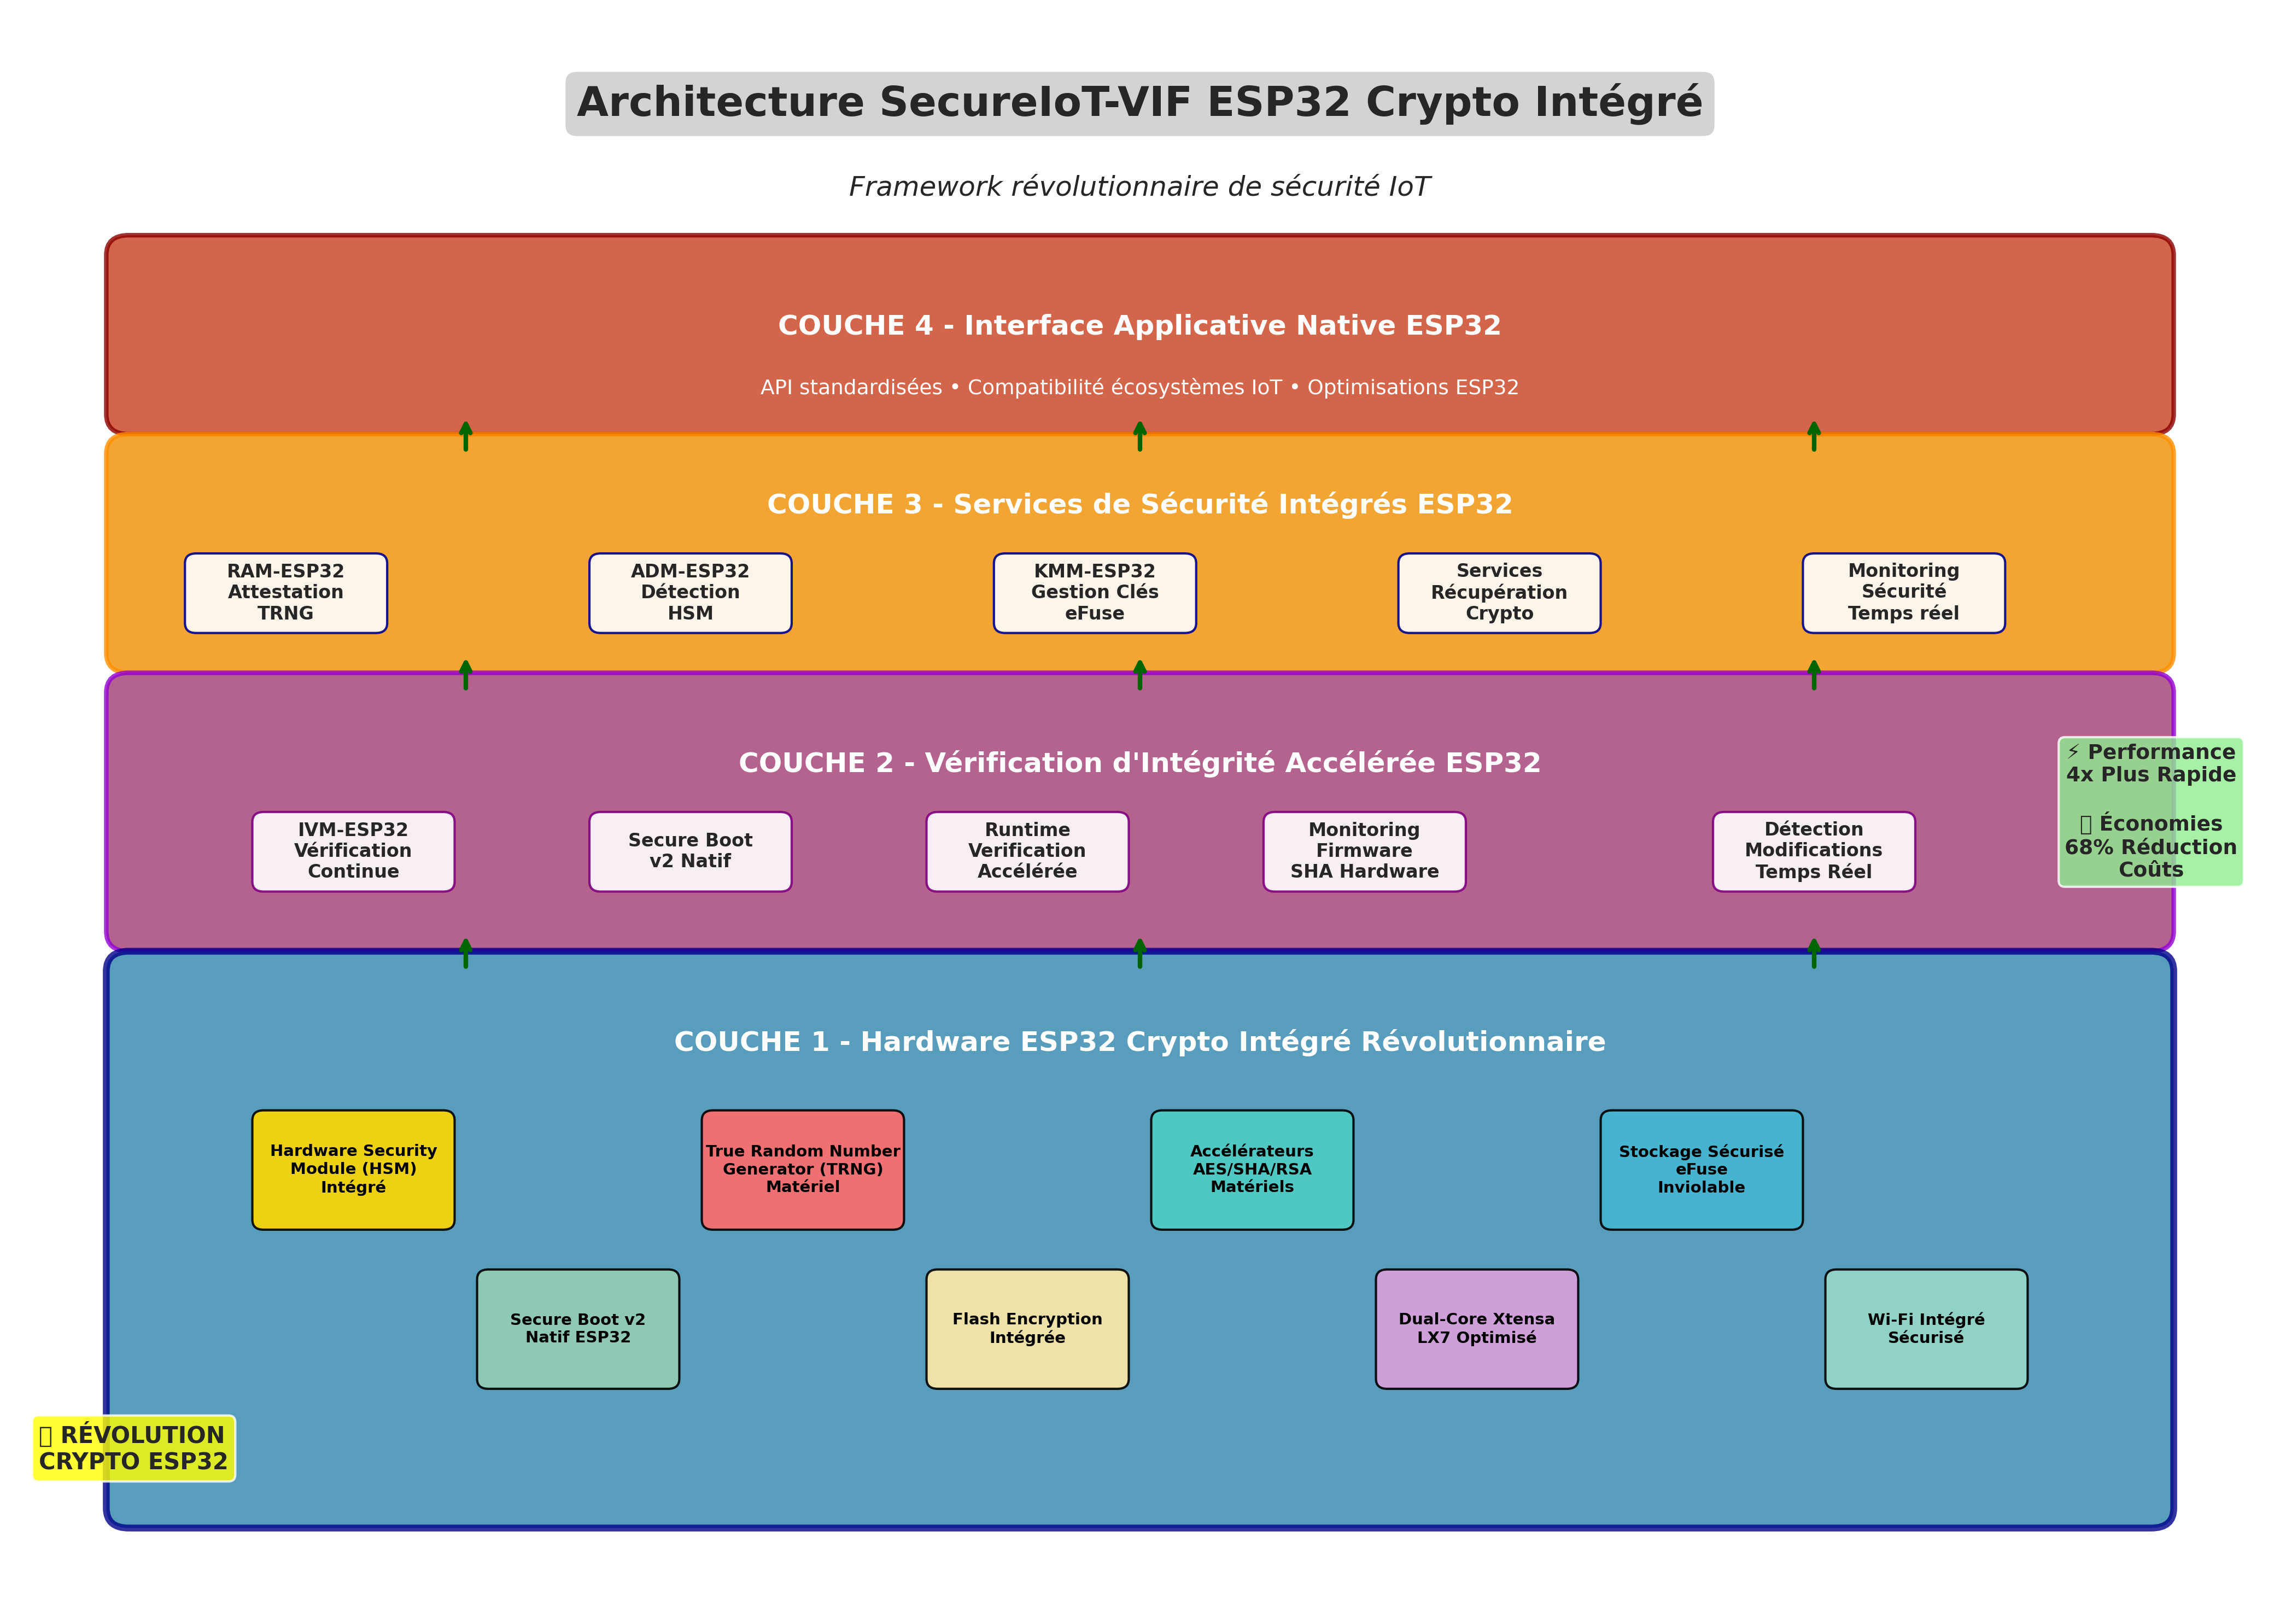
\includegraphics[width=0.9\textwidth]{assets/figures/secureiot_architecture_esp32.png}
    \caption{Architecture de SecureIoT-VIF Community Edition}
    \label{fig:secureiot-architecture-community}
\end{figure}

\textbf{Couche cryptographique de base :} Cette couche fondamentale comprend les opérations cryptographiques software utilisant mbedTLS : génération de clés, calculs de hash SHA-256, signatures ECDSA, et génération de nombres aléatoires. Elle fournit les primitives de sécurité de base compréhensibles et auditables.

\textbf{Couche de vérification d'intégrité de base :} Cette couche implémente les mécanismes de vérification d'intégrité du firmware adaptés à l'apprentissage, incluant la vérification au démarrage et le monitoring périodique simple. Elle s'appuie sur les services cryptographiques de base pour des opérations éducatives transparentes.

\textbf{Couche de services de sécurité éducatifs :} Cette couche fournit les services de sécurité de niveau intermédiaire : détection d'anomalies par seuils fixes, gestion basique des clés, et logging des événements de sécurité. Elle orchestre les interactions entre les différents composants de manière compréhensible.

\textbf{Couche d'interface éducative :} Cette couche expose les services de sécurité aux applications éducatives et aux outils de démonstration via des API simples et bien documentées. Elle assure la compatibilité avec les environnements d'apprentissage et les exercices pratiques.

\section{Composants principaux éducatifs}

\subsection{Module de vérification d'intégrité basique (IVM-Basic)}

Le Module de Vérification d'Intégrité Basique constitue le cœur éducatif de SecureIoT-VIF Community Edition. Il implémente les mécanismes de vérification cryptographique de l'intégrité du firmware de manière compréhensible et progressive.

\subsubsection{Vérification au démarrage éducative}

Le processus de démarrage sécurisé établit une chaîne de confiance simple depuis le bootloader jusqu'au firmware applicatif. Cette approche utilise des concepts cryptographiques de base facilement compréhensibles.

\textbf{Étape 1 - Initialisation de la cryptographie de base :} Le processus démarre par l'initialisation de mbedTLS et la configuration des algorithmes cryptographiques software. Cette étape est entièrement transparente et loggée pour l'apprentissage.

\textbf{Étape 2 - Vérification du bootloader :} Le bootloader principal est vérifié cryptographiquement avant son exécution en utilisant des signatures ECDSA software. Cette vérification démontre les concepts de base de la chaîne de confiance.

\textbf{Étape 3 - Vérification du kernel :} Le kernel du système d'exploitation embarqué est vérifié selon le même processus éducatif, établissant une chaîne de confiance compréhensible.

\textbf{Étape 4 - Vérification du firmware applicatif :} Le firmware applicatif principal est vérifié et son intégrité est attestée avant le démarrage des services utilisateur, démontrant l'application pratique des concepts.

\subsubsection{Vérification périodique éducative (Runtime Monitoring Basic)}

Contrairement aux approches qui ne vérifient l'intégrité qu'au démarrage, SecureIoT-VIF Community Edition implémente une vérification périodique pendant l'exécution, adaptée aux contraintes éducatives et à la compréhension progressive.

\textbf{Mécanisme de hachage par blocs :} Le firmware est divisé en blocs de taille éducative (4 KB) et chaque bloc est haché périodiquement en utilisant SHA-256 software. Cette approche permet de comprendre les concepts de vérification d'intégrité sans complexité excessive.

\textbf{Vérification basée sur un calendrier fixe :} La vérification suit un calendrier prévisible et configurable (toutes les 5 minutes par défaut) permettant aux étudiants d'observer et de comprendre le processus.

\textbf{Optimisation éducative :} La vérification utilise un seul cœur de l'ESP32 avec des algorithmes simples pour minimiser l'impact sur les performances tout en maintenant la transparence éducative.

\subsection{Module de détection d'anomalies éducatif (ADM-Basic)}

Le Module de Détection d'Anomalies Éducatif implémente des techniques de détection par seuils fixes pour identifier les comportements anormaux sans nécessiter de connaissances avancées en apprentissage automatique.

\subsubsection{Collecte de métriques comportementales simples}

\textbf{Métriques de performance de base :} Analyse de l'utilisation CPU, de la mémoire disponible, et de la température pour détecter les déviations du comportement normal en utilisant des seuils fixes compréhensibles.

\textbf{Métriques de ressources éducatives :} Surveillance de l'utilisation des ressources système pour identifier les consommations anormales indicatrices d'activité malveillante, avec des seuils configurables pour l'apprentissage.

\textbf{Métriques de communication de base :} Analyse simple des patterns de communication réseau pour détecter les communications suspectes, en utilisant des règles basiques facilement compréhensibles.

\subsubsection{Algorithmes de détection par seuils fixes}

\textbf{Détection par seuils statiques :} Utilisation d'algorithmes de détection basés sur des seuils fixes configurables pour identifier les patterns anormaux et détecter les déviations du comportement attendu.

\textbf{Analyse temporelle simple :} Prise en compte de la dimension temporelle dans l'analyse des comportements en utilisant des fenêtres glissantes simples pour détecter les anomalies persistantes.

\textbf{Règles de décision transparentes :} Implémentation de règles de décision explicites et configurables permettant aux étudiants de comprendre le processus de détection et d'ajuster les paramètres pour l'expérimentation.

\subsection{Module de gestion des clés éducatif (KMM-Basic)}

Le Module de Gestion des Clés Éducatif assure la génération, le stockage, et la gestion des clés cryptographiques en utilisant des mécanismes software compréhensibles.

\subsubsection{Hiérarchie des clés éducative}

\textbf{Clé racine software :} Stockée dans la mémoire flash de l'ESP32 avec protection logicielle, cette clé sert à dériver les autres clés en utilisant des fonctions de dérivation standard (HKDF).

\textbf{Clés d'intégrité dérivées :} Utilisées pour les calculs de hash SHA-256 et la vérification d'intégrité, dérivées de la clé racine selon un processus transparent et éducatif.

\textbf{Clés de signature temporaires :} Utilisées pour signer les événements de sécurité et les rapports d'état, renouvelées périodiquement selon un processus observable.

\textbf{Clés de communication basiques :} Utilisées pour les communications sécurisées simples, gérées selon des protocoles de base facilement compréhensibles.

\subsubsection{Protocoles de gestion éducatifs}

\textbf{Génération sécurisée software :} Utilisation du générateur de nombres aléatoires software de mbedTLS pour assurer une entropie suffisante des clés avec transparence éducative.

\textbf{Stockage sécurisé software :} Les clés sensibles sont stockées dans la mémoire flash avec protection software, démontrant les concepts de base de la protection des clés.

\textbf{Rotation manuelle :} Mécanisme de rotation des clés activable manuellement pour permettre l'expérimentation et la compréhension des concepts de gestion des clés.

\section{Protocoles de sécurité éducatifs}

\subsection{Protocole de démarrage sécurisé éducatif}

Le protocole de démarrage sécurisé éducatif de SecureIoT-VIF Community Edition établit une chaîne de confiance compréhensible tout en minimisant la complexité pour l'apprentissage.

\begin{algorithm}
\caption{Protocole de démarrage sécurisé éducatif}
\label{alg:secure-boot-educational}
\begin{algorithmic}[1]
\State \textbf{Initialisation cryptographique de base}
\State $mbedTLS \leftarrow$ mbedtls\_init()
\State $entropy \leftarrow$ mbedtls\_entropy\_init()
\State $État \leftarrow$ CRYPTO\_INITIALIZING

\State \textbf{Vérification du bootloader software}
\State $Signature_{BL} \leftarrow$ read\_bootloader\_signature()
\State $Hash_{BL} \leftarrow$ mbedtls\_sha256(bootloader\_data)
\If{mbedtls\_ecdsa\_verify($Hash_{BL}$, $Signature_{BL}$)}
    \State $État \leftarrow$ BOOTLOADER\_VERIFIED
    \State log\_educational\_event("Bootloader vérifié avec succès")
\Else
    \State log\_educational\_error("Échec vérification bootloader")
    \State \textbf{return} VERIFICATION\_FAILED
\EndIf

\State \textbf{Vérification du firmware applicatif}
\State $Signature_{App} \leftarrow$ read\_application\_signature()
\State $Hash_{App} \leftarrow$ mbedtls\_sha256(application\_data)
\If{mbedtls\_ecdsa\_verify($Hash_{App}$, $Signature_{App}$)}
    \State $État \leftarrow$ APPLICATION\_VERIFIED
    \State log\_educational\_event("Application vérifiée avec succès")
    \State \textbf{return} VERIFICATION\_SUCCESS
\Else
    \State log\_educational\_error("Échec vérification application")
    \State \textbf{return} VERIFICATION\_FAILED
\EndIf
\end{algorithmic}
\end{algorithm}

\subsection{Protocole de vérification périodique éducative}

La vérification périodique représente une innovation pédagogique majeure de SecureIoT-VIF Community Edition, permettant la compréhension des concepts de vérification continue.

\begin{algorithm}
\caption{Protocole de vérification périodique éducative}
\label{alg:periodic-verification-educational}
\begin{algorithmic}[1]
\State \textbf{Initialisation éducative}
\State $Blocs \leftarrow$ firmware\_partition / FIRMWARE\_CHUNK\_SIZE
\State $Hashes\_Référence \leftarrow$ calculate\_reference\_hashes($Blocs$)
\State $Scheduler \leftarrow$ create\_simple\_scheduler()

\State \textbf{Boucle de vérification éducative}
\While{$system\_healthy() == true$}
    \State $Bloc\_Actuel \leftarrow$ Scheduler.select\_next\_block()
    \State $Hash\_Actuel \leftarrow$ mbedtls\_sha256($Bloc\_Actuel$)
    \State $Hash\_Référence \leftarrow$ get\_reference\_hash($Bloc\_Actuel$)
    
    \If{$Hash\_Actuel \neq Hash\_Référence$}
        \State $Anomalie \leftarrow$ detect\_integrity\_violation()
        \State log\_educational\_alert("Violation d'intégrité détectée", $Bloc\_Actuel$)
        \State trigger\_educational\_response($Anomalie$)
    \Else
        \State log\_educational\_event("Bloc vérifié OK", $Bloc\_Actuel$)
    \EndIf
    
    \State wait\_educational\_interval(VERIFICATION\_INTERVAL\_MS)
\EndWhile
\end{algorithmic}
\end{algorithm}

\subsection{Protocole de détection d'anomalies éducatif}

Le protocole de détection d'anomalies éducatif permet aux étudiants de comprendre les mécanismes de base de la détection comportementale sans complexité excessive.

\begin{algorithm}
\caption{Protocole de détection d'anomalies par seuils éducatif}
\label{alg:anomaly-detection-educational}
\begin{algorithmic}[1]
\State \textbf{Collecte des métriques éducatives}
\State $CPU\_Usage \leftarrow$ get\_cpu\_usage\_percentage()
\State $Memory\_Free \leftarrow$ get\_free\_memory\_kb()
\State $Temperature \leftarrow$ get\_system\_temperature()
\State $Network\_Activity \leftarrow$ get\_network\_packets\_per\_second()

\State \textbf{Évaluation par seuils fixes éducatifs}
\If{$CPU\_Usage > CPU\_THRESHOLD\_HIGH$}
    \State log\_educational\_anomaly("CPU usage élevé", $CPU\_Usage$)
    \State $Anomaly\_Score \leftarrow$ $Anomaly\_Score$ + 1
\EndIf

\If{$Memory\_Free < MEMORY\_THRESHOLD\_LOW$}
    \State log\_educational\_anomaly("Mémoire faible", $Memory\_Free$)
    \State $Anomaly\_Score \leftarrow$ $Anomaly\_Score$ + 1
\EndIf

\If{$Temperature > TEMPERATURE\_THRESHOLD$}
    \State log\_educational\_anomaly("Température élevée", $Temperature$)
    \State $Anomaly\_Score \leftarrow$ $Anomaly\_Score$ + 1
\EndIf

\State \textbf{Décision éducative simple}
\If{$Anomaly\_Score \geq ANOMALY\_THRESHOLD$}
    \State trigger\_educational\_alert("Anomalie comportementale détectée")
    \State \textbf{return} ANOMALY\_DETECTED
\Else
    \State \textbf{return} SYSTEM\_NORMAL
\EndIf
\end{algorithmic}
\end{algorithm}

\section{Mécanismes d'optimisation éducatifs}

\subsection{Optimisations cryptographiques éducatives}

\subsubsection{Utilisation efficace de mbedTLS}

SecureIoT-VIF Community Edition optimise l'utilisation de la bibliothèque mbedTLS pour l'éducation :

\textbf{Signatures numériques éducatives :} ECDSA P-256 via mbedTLS pour les signatures compréhensibles et les vérifications transparentes, Ed25519 pour la compatibilité moderne, avec logging détaillé des opérations pour l'apprentissage.

\textbf{Fonctions de hachage software :} SHA-256 via mbedTLS pour les calculs d'intégrité transparents, BLAKE2s pour les opérations spécialisées éducatives, avec possibilité de traçage pour l'apprentissage.

\textbf{Chiffrement symétrique éducatif :} AES-256 via mbedTLS pour les communications sécurisées de base, ChaCha20-Poly1305 pour les démonstrations avancées, avec interfaces de débogage pour la compréhension.

\subsubsection{Optimisations software éducatives}

\textbf{Calculs séquentiels compréhensibles :} Utilisation d'algorithmes séquentiels facilement compréhensibles plutôt que de parallélisation complexe, permettant aux étudiants de suivre le flot d'exécution.

\textbf{Optimisations mémoire transparentes :} Algorithmes de hachage en streaming optimisés pour l'ESP32 mais conservant la lisibilité du code pour l'apprentissage.

\textbf{Logging éducatif détaillé :} Instrumentation complète du code pour permettre aux étudiants de comprendre chaque étape des processus cryptographiques.

\subsection{Optimisations énergétiques éducatives}

\subsubsection{Gestion adaptative de la puissance éducative}

\textbf{Ordonnancement adaptatif simple :} Ajustement de la fréquence de vérification en fonction de l'état de la batterie selon des règles simples et compréhensibles.

\textbf{Modes de veille éducatifs :} Suspension coordonnée des vérifications non critiques pendant les périodes d'inactivité, avec possibilité d'observation du comportement.

\textbf{Optimisation des communications :} Agrégation des messages de logging et utilisation intelligente des modes d'économie d'énergie pour réduire la consommation radio.

\section{Adaptation aux contraintes éducatives}

\subsection{Gestion des ressources éducatives}

\subsubsection{Adaptation dynamique simple}

SecureIoT-VIF Community Edition implémente des mécanismes d'adaptation simples pour fonctionner efficacement sur des plateformes éducatives contraintes :

\textbf{Profilage des ressources automatique :} Évaluation simple des ressources disponibles (CPU, RAM, Flash) au démarrage avec affichage des limitations pour l'apprentissage.

\textbf{Configuration adaptative transparente :} Ajustement automatique des paramètres de sécurité en fonction des ressources disponibles avec explication des choix effectués.

\textbf{Dégradation gracieuse éducative :} Réduction progressive des fonctionnalités de sécurité en cas de contraintes sévères, avec explication pédagogique des compromis nécessaires.

\subsection{Compatibilité éducative multi-plateforme}

\subsubsection{Abstraction matérielle éducative}

\textbf{Couche d'abstraction cryptographique :} Interface standardisée pour accéder aux capacités cryptographiques de base de différentes plateformes éducatives (ESP32, Arduino, Raspberry Pi).

\textbf{Abstraction des primitives de base :} API unifiée pour les opérations cryptographiques software s'adaptant aux différentes implémentations de mbedTLS disponibles.

\textbf{Abstraction du système d'exploitation éducative :} Compatibilité avec FreeRTOS, Linux embarqué, et autres OS éducatifs populaires.

\section{Sécurité du framework éducatif}

\subsection{Analyse de sécurité éducative}

\subsubsection{Résistance aux attaques éducatives}

SecureIoT-VIF Community Edition est conçu pour résister aux principales menaces éducatives identifiées :

\textbf{Attaques par injection de malware éducatif :} La vérification périodique détecte les modifications de firmware en temps acceptable (< 5 minutes), permettant une démonstration efficace des concepts de détection.

\textbf{Attaques par modification de données :} Les mécanismes de vérification d'intégrité par blocs permettent de localiser précisément les modifications, offrant une excellente valeur pédagogique.

\textbf{Attaques par surcharge de ressources :} La détection par seuils fixes identifie les consommations anormales de ressources, démontrant les concepts de détection comportementale.

\subsubsection{Propriétés de sécurité éducatives}

\textbf{Intégrité de base :} Garantie que le firmware n'a pas été modifié de manière non autorisée, vérifiée périodiquement avec granularité éducative.

\textbf{Authenticité éducative :} Vérification que le firmware provient d'une source légitime, avec possibilité de traçage pour l'apprentissage.

\textbf{Détectabilité transparente :} Assurance que les modifications malveillantes sont détectées dans un délai raisonnable pour l'expérimentation éducative.

\subsection{Mécanismes de récupération éducatifs}

\subsubsection{Détection et réponse pédagogiques}

\textbf{Détection observable :} Identification des compromissions par analyse comportementale simple et vérification d'intégrité périodique avec logging détaillé pour l'apprentissage.

\textbf{Réponse éducative configurée :} Actions de réponse configurables permettant l'expérimentation avec différents niveaux de sévérité et types de contre-mesures.

\textbf{Logging éducatif complet :} Enregistrement détaillé de tous les événements de sécurité avec horodatage et contexte pour l'analyse post-incident éducative.

\section{Conclusion}

Ce chapitre a présenté la conception complète de SecureIoT-VIF Community Edition, notre framework éducatif de vérification d'intégrité pour les firmwares IoT. L'architecture proposée combine plusieurs innovations éducatives :

\begin{itemize}
    \item Une approche de vérification périodique compréhensible permettant l'apprentissage des concepts de monitoring en temps réel
    \item L'utilisation efficace de la cryptographie software (mbedTLS) pour des opérations transparentes et auditables
    \item Des mécanismes de détection d'anomalies par seuils fixes, facilement compréhensibles et configurables
    \item Des mécanismes d'adaptation dynamique aux ressources éducatives disponibles avec transparence pédagogique
    \item Une architecture modulaire facilitant la compréhension progressive des concepts de sécurité IoT
\end{itemize}

La conception présentée répond aux exigences éducatives identifiées dans l'analyse des besoins tout en respectant les contraintes d'accessibilité et de simplicité nécessaires à un usage pédagogique efficace. Le chapitre suivant détaille l'implémentation concrète de ces concepts sur la plateforme ESP32, validant la faisabilité pratique de l'approche proposée et démontrant son efficacité pour l'enseignement de la sécurité IoT.
%====================================================================
% Chapitre 5 : Implémentation de SecureIoT-VIF Community Edition
%====================================================================

\chapter{Implémentation de SecureIoT-VIF Community Edition}
\label{chap:implementation}

\section{Introduction}

Ce chapitre présente l'implémentation concrète du framework SecureIoT-VIF Community Edition dans le cadre de notre approche éducative. L'implémentation privilégie la simplicité, la compréhensibilité et l'accessibilité financière sur la plateforme ESP32 (~8$) en utilisant exclusivement de la cryptographie software (mbedTLS). Cette méthodologie permet de valider les concepts de conception éducative tout en démontrant la faisabilité pratique du framework sur une plateforme contrainte accessible aux établissements d'enseignement et aux projets de recherche avec des budgets limités.

\section{Architecture d'implémentation éducative}

\subsection{Vue d'ensemble technique accessible}

L'implémentation de SecureIoT-VIF Community Edition suit une architecture modulaire simple, spécifiquement conçue pour l'accessibilité éducative et la compréhension progressive des concepts de sécurité IoT.

\begin{figure}[h]
    \centering
    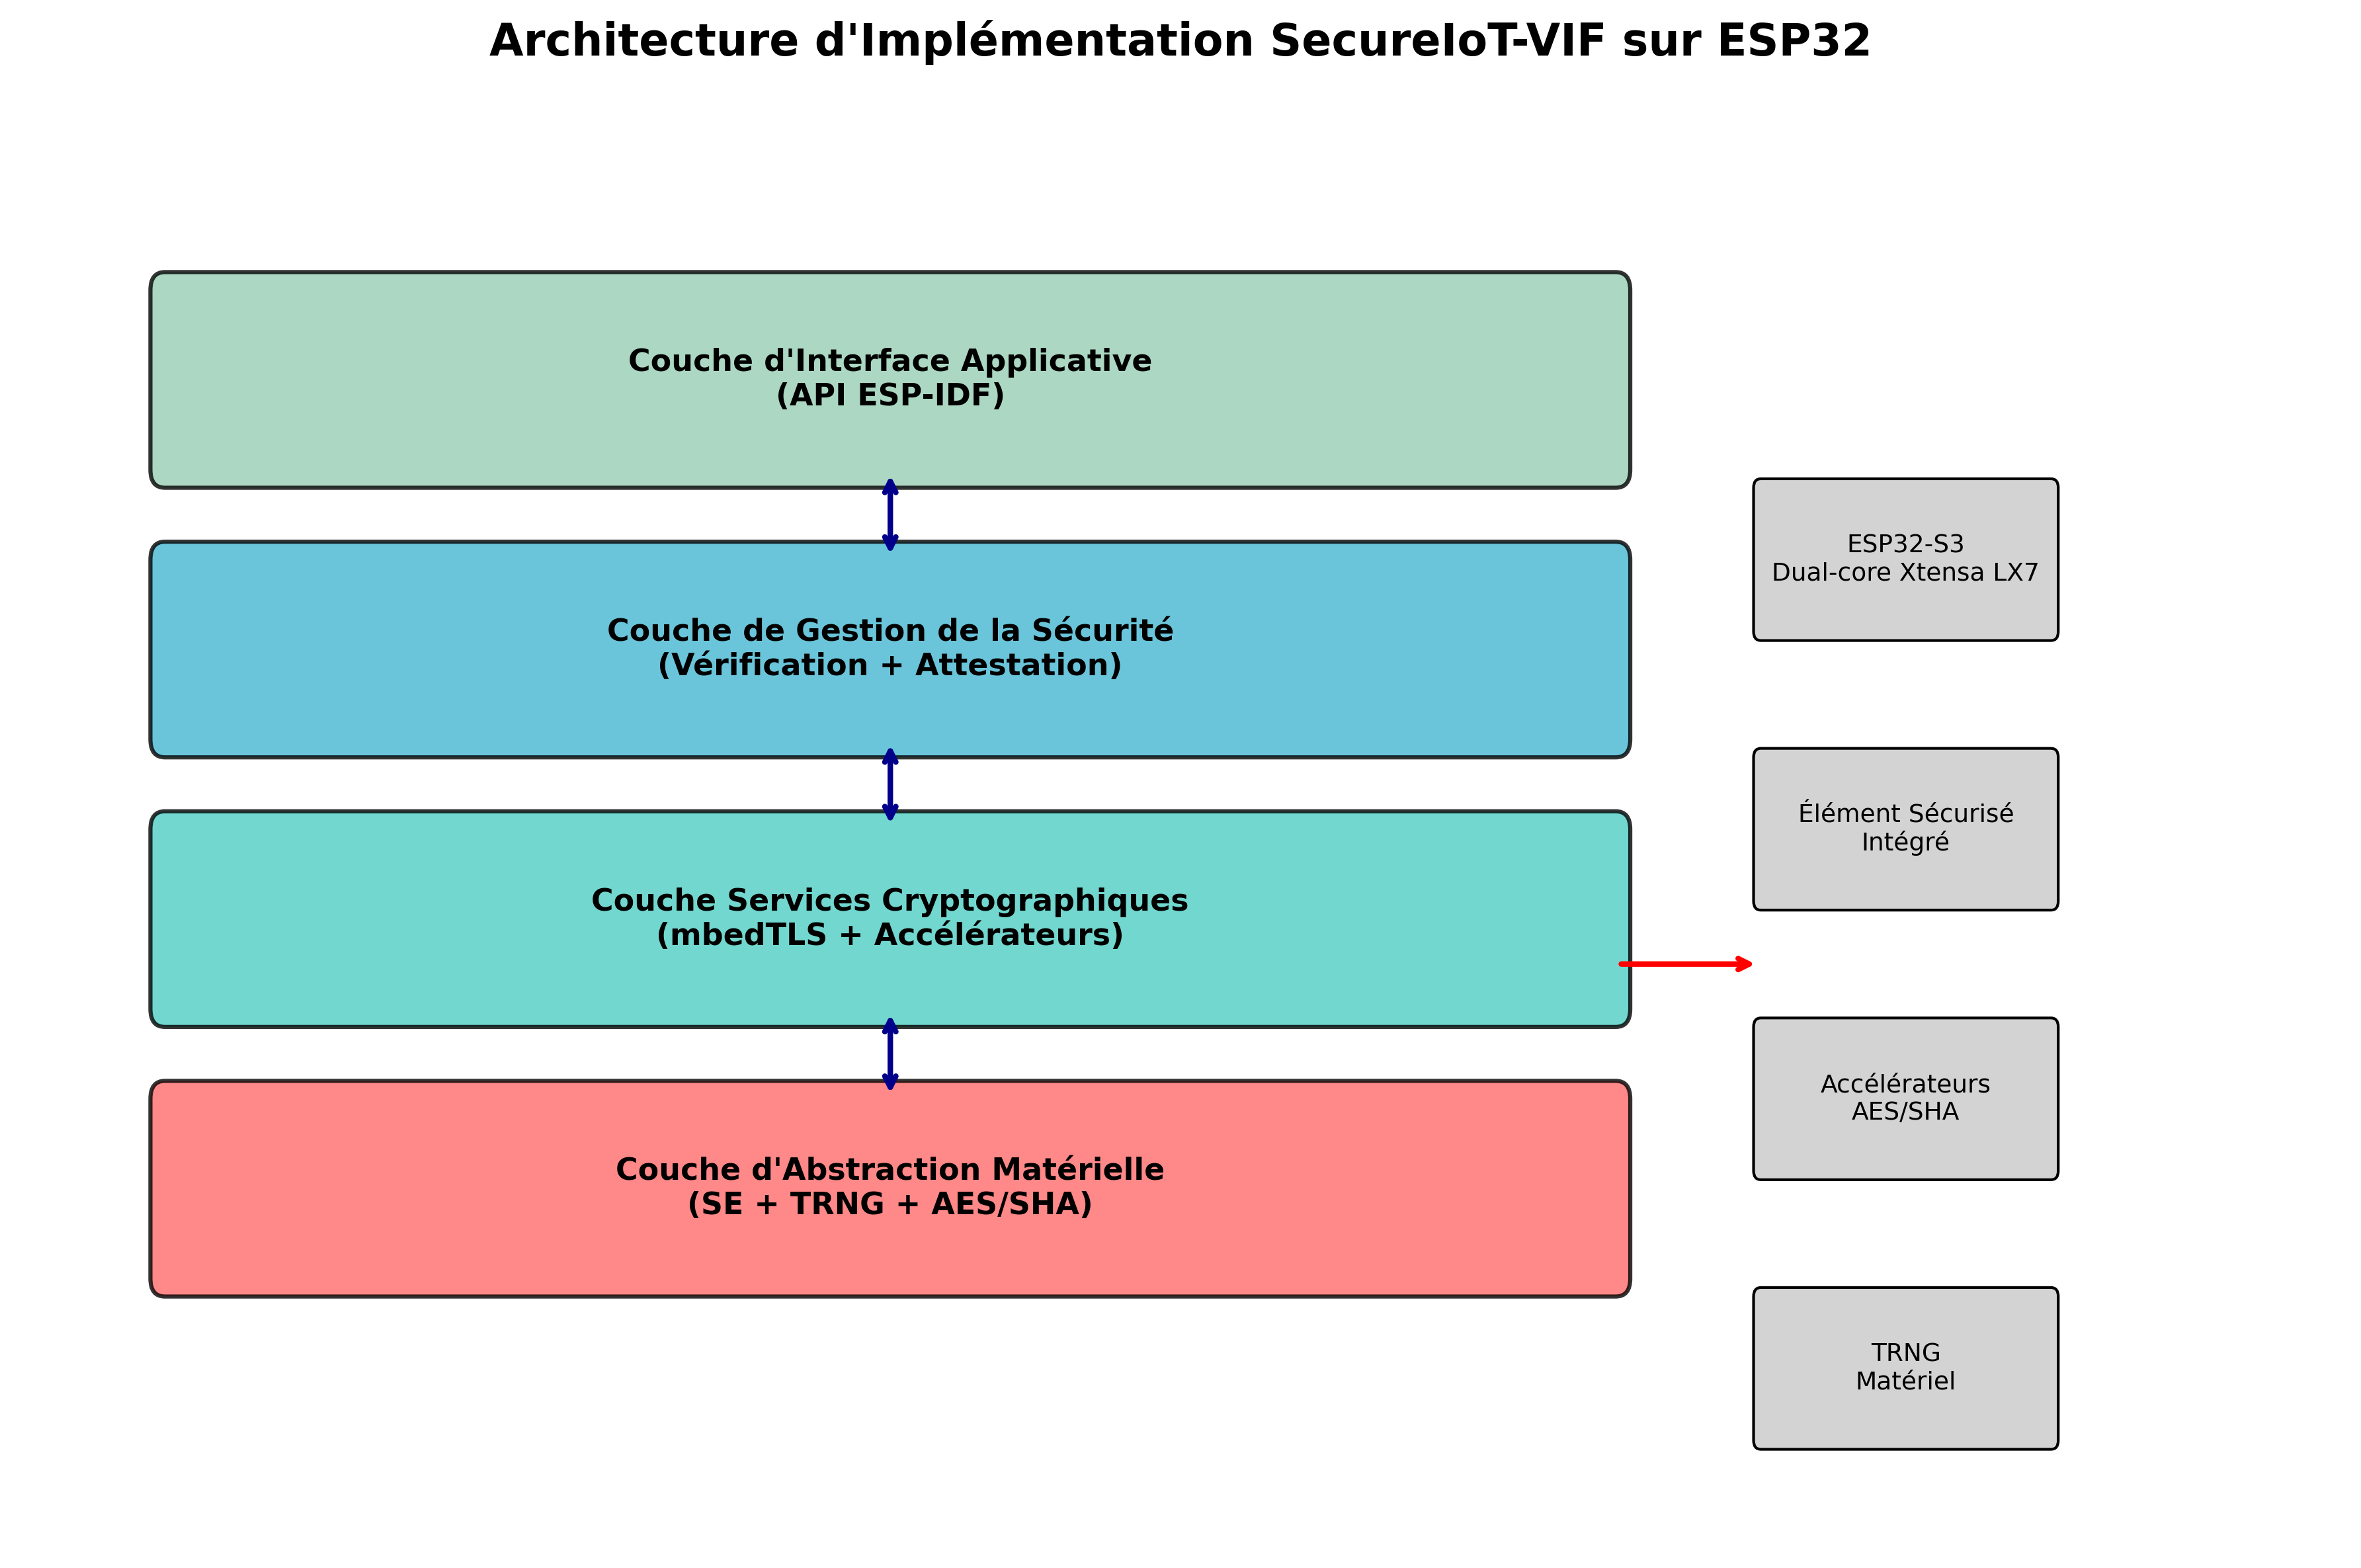
\includegraphics[width=0.9\textwidth]{assets/figures/implementation_architecture_esp32.png}
    \caption{Architecture d'implémentation SecureIoT-VIF Community Edition}
    \label{fig:implementation-architecture-community}
\end{figure}

\textbf{Couche d'abstraction matérielle éducative (HAL) :} Interface unifiée simple exploitant les ressources de base de l'ESP32 : processeur dual-core Xtensa LX6, 512KB SRAM, 16MB Flash, et périphériques de base (GPIO, UART, Wi-Fi).

\textbf{Couche de services cryptographiques software :} Implémentation transparente des primitives cryptographiques utilisant exclusivement mbedTLS pour des opérations auditables et compréhensibles.

\textbf{Couche de gestion de la sécurité éducative :} Orchestration simple des mécanismes de vérification d'intégrité et de détection d'anomalies, adaptée aux contraintes pédagogiques et optimisée pour la compréhension.

\textbf{Couche d'interface éducative :} API légère exposant les services de SecureIoT-VIF Community aux applications éducatives et aux exercices pratiques, maximisant la lisibilité du code.

\subsection{Choix technologiques éducatifs}

\subsubsection{Environnement de développement accessible}

\textbf{ESP-IDF (Espressif IoT Development Framework) :} Framework officiel choisi pour sa documentation complète, sa communauté active, et son excellent support de mbedTLS intégré.

\textbf{FreeRTOS éducatif :} Système d'exploitation temps réel simple, permettant l'ordonnancement coopératif des tâches de vérification avec les applications utilisateur de manière transparente.

\textbf{Toolchain GCC standard :} Compilateur standard pour l'architecture Xtensa, largement disponible et bien documenté pour l'apprentissage.

\subsubsection{Bibliothèques cryptographiques éducatives}

\textbf{mbedTLS intégré :} Utilisation exclusive de la bibliothèque mbedTLS fournie avec ESP-IDF pour toutes les opérations cryptographiques, garantissant la transparence et l'auditabilité.

\textbf{Implémentations software uniquement :} Évitement délibéré des accélérateurs matériels pour privilégier la compréhension des algorithmes et la portabilité éducative.

\textbf{Logging éducatif détaillé :} Instrumentation complète du code pour permettre le suivi et la compréhension de chaque opération cryptographique.

\section{Implémentation détaillée sur ESP32}

\subsection{Spécifications de la plateforme éducative}

\subsubsection{Caractéristiques matérielles exploitées}

L'ESP32-WROOM-32 utilisé pour l'implémentation Community présente les caractéristiques suivantes :

\begin{table}[h]
\centering
\caption{Spécifications ESP32 pour SecureIoT-VIF Community Edition}
\label{tab:esp32-community-specs}
\begin{tabular}{|l|c|c|}
\hline
\textbf{Composant} & \textbf{Spécification} & \textbf{Coût approximatif} \\
\hline
ESP32-WROOM-32 & Dual-core Xtensa LX6 @ 240 MHz & ~5\$ \\
SRAM & 512 KB total & Inclus \\
Flash & 16 MB (optionnel 4MB min) & +0\$ (4MB) / +1\$ (16MB) \\
DHT22 & Capteur température/humidité & ~3\$ \\
Connecteurs & Breadboard + câbles & ~0\$ (matériel de base) \\
\hline
\textbf{Coût total} & \textbf{Système complet} & \textbf{~8\$} \\
\hline
\end{tabular}
\end{table}

\subsection{Architecture logicielle éducative détaillée}

\subsubsection{Répartition des tâches éducative}

L'ESP32 dual-core permet une répartition simple et compréhensible des charges :

\textbf{Core 0 (Protocol CPU) :}
\begin{itemize}
    \item Applications utilisateur éducatives
    \item Communications réseau Wi-Fi de base
    \item Interface API SecureIoT-VIF simple
    \item Gestion des interruptions système
\end{itemize}

\textbf{Core 1 (Application CPU) :}
\begin{itemize}
    \item Tâches de vérification d'intégrité periodiques
    \item Détection d'anomalies par seuils fixes
    \item Opérations cryptographiques software via mbedTLS
    \item Logging et monitoring éducatif
\end{itemize}

\subsection{Modules d'implémentation éducatifs principaux}

\subsubsection{Module de vérification d'intégrité éducatif (IVM-Community)}

\lstset{language=C}
\begin{lstlisting}[caption={Implémentation IVM Community utilisant mbedTLS}]
#include "esp_system.h"
#include "esp_flash.h"
#include "mbedtls/sha256.h"         // Crypto software uniquement
#include "mbedtls/ecdsa.h"          // Signatures software
#include "freertos/FreeRTOS.h"
#include "freertos/task.h"

// Configuration éducative de vérification Community Edition
typedef struct {
    size_t block_size;              // 4KB pour granularité éducative
    uint32_t verification_interval; // 5 minutes pour apprentissage
    bool software_crypto_only;      // Toujours true en Community
    uint8_t core_affinity;          // Core 1 dédié sécurité
} secureiot_community_ivm_config_t;

// Structure de hash par bloc éducative
typedef struct {
    uint32_t block_id;
    uint8_t hash[32];               // SHA-256 standard
    uint32_t timestamp;
    bool verified;
    char description[64];           // Description éducative
} secureiot_community_block_hash_t;

// Cache de hashes pour optimisation éducative
#define MAX_CACHED_BLOCKS 128      // Limité pour contraintes éducatives
static secureiot_community_block_hash_t hash_cache[MAX_CACHED_BLOCKS];
static size_t cache_size = 0;
static SemaphoreHandle_t cache_mutex;

// Initialisation éducative du module IVM Community
esp_err_t secureiot_community_ivm_init(
    secureiot_community_ivm_config_t* config) {
    esp_err_t ret = ESP_OK;
    
    ESP_LOGI(TAG, "🎓 Initializing SecureIoT-VIF Community Edition");
    ESP_LOGI(TAG, "📚 Educational framework - Software crypto only");
    
    // Création du mutex pour protection cache éducative
    cache_mutex = xSemaphoreCreateMutex();
    if (cache_mutex == NULL) {
        ESP_LOGE(TAG, "❌ Failed to create educational cache mutex");
        return ESP_ERR_NO_MEM;
    }
    
    // Initialisation mbedTLS pour éducation
    mbedtls_sha256_context sha256_ctx;
    mbedtls_sha256_init(&sha256_ctx);
    
    // Test éducatif de mbedTLS
    uint8_t test_data[] = "SecureIoT-VIF Community Test";
    uint8_t test_hash[32];
    int mbedtls_ret = mbedtls_sha256_ret(test_data, strlen((char*)test_data), 
                                        test_hash, 0);
    
    if (mbedtls_ret != 0) {
        ESP_LOGE(TAG, "❌ mbedTLS initialization failed: -0x%04x", -mbedtls_ret);
        return ESP_FAIL;
    }
    
    ESP_LOGI(TAG, "✅ mbedTLS initialized successfully for education");
    
    // Calcul initial des hashes de référence éducatifs
    ret = secureiot_calculate_reference_hashes_community();
    if (ret != ESP_OK) {
        ESP_LOGE(TAG, "❌ Failed to calculate educational reference hashes");
        return ret;
    }
    
    ESP_LOGI(TAG, "🎉 Community IVM initialized with %d cached blocks", cache_size);
    ESP_LOGI(TAG, "💡 Ideal for learning IoT security concepts!");
    
    return ESP_OK;
}

// Vérification éducative d'intégrité par bloc avec mbedTLS
esp_err_t secureiot_community_verify_block(uint32_t block_id) {
    esp_err_t ret = ESP_OK;
    uint8_t calculated_hash[32];
    uint8_t reference_hash[32];
    
    ESP_LOGD(TAG, "🔍 Verifying educational block %lu with software crypto", block_id);
    
    // Calcul du hash avec mbedTLS (software uniquement)
    ret = secureiot_calculate_block_hash_mbedtls(block_id, calculated_hash);
    if (ret != ESP_OK) {
        ESP_LOGE(TAG, "❌ Educational hash calculation failed for block %lu", block_id);
        return ret;
    }
    
    // Récupération du hash de référence depuis cache éducatif
    ret = secureiot_get_reference_hash_community(block_id, reference_hash);
    if (ret != ESP_OK) {
        ESP_LOGW(TAG, "⚠️  Reference hash not found for block %lu (educational)", block_id);
        return ret;
    }
    
    // Comparaison éducative transparente des hashes
    if (memcmp(calculated_hash, reference_hash, 32) != 0) {
        ESP_LOGW(TAG, "🚨 Educational integrity violation detected in block %lu", block_id);
        ESP_LOGW(TAG, "💡 This is an excellent learning opportunity!");
        return ESP_ERR_INVALID_CRC;
    }
    
    // Mise à jour du cache éducatif
    if (xSemaphoreTake(cache_mutex, pdMS_TO_TICKS(100)) == pdTRUE) {
        secureiot_update_hash_cache_community(block_id, calculated_hash);
        xSemaphoreGive(cache_mutex);
    }
    
    ESP_LOGD(TAG, "✅ Educational block %lu verified successfully", block_id);
    return ESP_OK;
}

// Calcul éducatif de hash avec mbedTLS pur
esp_err_t secureiot_calculate_block_hash_mbedtls(uint32_t block_id, 
                                                uint8_t* hash) {
    const size_t BLOCK_SIZE = FIRMWARE_CHUNK_SIZE;  // 4KB éducatif
    uint8_t block_buffer[BLOCK_SIZE];
    
    ESP_LOGD(TAG, "📊 Calculating educational hash for block %lu with mbedTLS", block_id);
    
    // Lecture éducative du bloc depuis la flash
    uint32_t block_addr = FIRMWARE_BASE_ADDR + (block_id * BLOCK_SIZE);
    esp_err_t ret = esp_flash_read(NULL, block_buffer, block_addr, BLOCK_SIZE);
    if (ret != ESP_OK) {
        ESP_LOGE(TAG, "❌ Failed to read educational block %lu: %s", 
                 block_id, esp_err_to_name(ret));
        return ret;
    }
    
    // Calcul SHA-256 éducatif avec mbedTLS (software uniquement)
    int mbedtls_ret = mbedtls_sha256_ret(block_buffer, BLOCK_SIZE, hash, 0);
    if (mbedtls_ret != 0) {
        ESP_LOGE(TAG, "❌ mbedTLS SHA256 failed for educational block %lu: -0x%04x", 
                 block_id, -mbedtls_ret);
        return ESP_FAIL;
    }
    
    ESP_LOGV(TAG, "✅ Educational SHA-256 completed for block %lu (software)", block_id);
    return ESP_OK;
}

// Tâche éducative de vérification continue Community
void secureiot_community_continuous_verification_task(void* parameter) {
    secureiot_community_ivm_config_t* config = 
        (secureiot_community_ivm_config_t*)parameter;
    
    // Affinité au Core 1 pour isolation éducative
    vTaskPinToCore(NULL, 1);
    
    uint32_t current_block = 0;
    uint32_t total_blocks = secureiot_get_total_firmware_blocks_community();
    TickType_t last_wake_time = xTaskGetTickCount();
    
    ESP_LOGI(TAG, "🎓 Community continuous verification task started on core 1");
    ESP_LOGI(TAG, "📚 Educational mode: software crypto only, 5-minute intervals");
    
    while (true) {
        // Vérification éducative adaptative basée sur la charge
        if (secureiot_get_system_load_community() < 80) {
            esp_err_t ret = secureiot_community_verify_block(current_block);
            if (ret != ESP_OK) {
                // Déclenchement d'alerte éducative
                ESP_LOGW(TAG, "🎓 Educational security event: integrity violation in block %lu", 
                         current_block);
                secureiot_trigger_educational_alert_community(current_block);
            } else {
                ESP_LOGD(TAG, "✅ Educational block %lu verification completed", current_block);
            }
            
            // Passage au bloc suivant avec wrap-around éducatif
            current_block = (current_block + 1) % total_blocks;
        } else {
            ESP_LOGD(TAG, "⏳ System load high, skipping verification (educational)");
        }
        
        // Attente éducative avec intervalle fixe (5 minutes)
        vTaskDelayUntil(&last_wake_time, 
                       pdMS_TO_TICKS(config->verification_interval));
    }
}
\end{lstlisting}

\subsubsection{Module de détection d'anomalies éducatif (ADM-Community)}

\begin{lstlisting}[caption={Module éducatif de détection d'anomalies par seuils}]
#include "esp_system.h"
#include "esp_timer.h"
#include "driver/temperature_sensor.h"

// Configuration éducative de détection d'anomalies Community
typedef struct {
    float temp_threshold_high;      // 50°C pour éducation
    float temp_threshold_low;       // 10°C pour éducation
    uint32_t cpu_threshold_high;    // 80% pour éducation
    uint32_t memory_threshold_low;  // 50KB pour éducation
    uint32_t detection_interval;    // 30s pour éducation
} secureiot_community_anomaly_config_t;

// Structure éducative de métriques système
typedef struct {
    uint32_t timestamp;
    float temperature;
    uint32_t cpu_usage_percent;
    uint32_t free_memory_kb;
    uint32_t free_flash_kb;
    bool wifi_connected;
    uint32_t network_packets_per_minute;
} __attribute__((packed)) secureiot_community_metrics_t;

// Historique éducatif des métriques (taille limitée)
#define COMMUNITY_METRICS_HISTORY_SIZE 50
static secureiot_community_metrics_t metrics_history[COMMUNITY_METRICS_HISTORY_SIZE];
static size_t metrics_history_index = 0;
static SemaphoreHandle_t metrics_mutex;

// Initialisation éducative du détecteur d'anomalies Community
esp_err_t secureiot_community_anomaly_detector_init(
    secureiot_community_anomaly_config_t* config) {
    
    ESP_LOGI(TAG, "🎓 Initializing Community anomaly detector (threshold-based)");
    ESP_LOGI(TAG, "📚 Educational approach: simple thresholds, no ML complexity");
    
    // Création du mutex pour protection des métriques éducatives
    metrics_mutex = xSemaphoreCreateMutex();
    if (metrics_mutex == NULL) {
        ESP_LOGE(TAG, "❌ Failed to create educational metrics mutex");
        return ESP_ERR_NO_MEM;
    }
    
    // Initialisation du capteur de température éducatif
    temperature_sensor_config_t temp_sensor_config = TEMPERATURE_SENSOR_CONFIG_DEFAULT(10, 50);
    temperature_sensor_handle_t temp_sensor = NULL;
    ESP_ERROR_CHECK(temperature_sensor_install(&temp_sensor_config, &temp_sensor));
    ESP_ERROR_CHECK(temperature_sensor_enable(temp_sensor));
    
    ESP_LOGI(TAG, "✅ Community anomaly detector initialized");
    ESP_LOGI(TAG, "💡 Thresholds: Temp %.1f-%.1fC, CPU <%d%%, Memory >%dKB", 
             config->temp_threshold_low, config->temp_threshold_high,
             config->cpu_threshold_high, config->memory_threshold_low);
    
    return ESP_OK;
}

// Collecte éducative des métriques système Community
esp_err_t secureiot_community_collect_metrics(
    secureiot_community_metrics_t* metrics) {
    
    ESP_LOGD(TAG, "📊 Collecting educational system metrics");
    
    // Horodatage éducatif
    metrics->timestamp = esp_timer_get_time() / 1000000; // secondes
    
    // Température éducative (si disponible)
    float temp_celsius;
    temperature_sensor_handle_t temp_sensor = NULL; // Récupérer depuis contexte global
    esp_err_t ret = temperature_sensor_get_celsius(temp_sensor, &temp_celsius);
    if (ret == ESP_OK) {
        metrics->temperature = temp_celsius;
        ESP_LOGD(TAG, "🌡️  Educational temperature: %.1f°C", temp_celsius);
    } else {
        metrics->temperature = 25.0f; // Valeur par défaut éducative
        ESP_LOGD(TAG, "🌡️  Using default educational temperature: 25.0°C");
    }
    
    // Utilisation CPU éducative (approximation simple)
    metrics->cpu_usage_percent = secureiot_get_cpu_usage_percentage_simple();
    ESP_LOGD(TAG, "💻 Educational CPU usage: %lu%%", metrics->cpu_usage_percent);
    
    // Mémoire libre éducative
    metrics->free_memory_kb = esp_get_free_heap_size() / 1024;
    ESP_LOGD(TAG, "💾 Educational free memory: %lu KB", metrics->free_memory_kb);
    
    // Flash libre éducative (approximation)
    metrics->free_flash_kb = secureiot_get_free_flash_size_kb_community();
    ESP_LOGD(TAG, "💿 Educational free flash: %lu KB", metrics->free_flash_kb);
    
    // État Wi-Fi éducatif
    wifi_ap_record_t ap_info;
    metrics->wifi_connected = (esp_wifi_sta_get_ap_info(&ap_info) == ESP_OK);
    ESP_LOGD(TAG, "📶 Educational WiFi: %s", 
             metrics->wifi_connected ? "Connected" : "Disconnected");
    
    // Trafic réseau éducatif (compteur simple)
    metrics->network_packets_per_minute = secureiot_get_network_activity_community();
    
    return ESP_OK;
}

// Détection éducative d'anomalies par seuils fixes
anomaly_result_t secureiot_community_detect_anomalies(
    secureiot_community_metrics_t* metrics,
    secureiot_community_anomaly_config_t* config) {
    
    anomaly_result_t result = {0};
    uint32_t anomaly_score = 0;
    char anomaly_details[256] = {0};
    
    ESP_LOGD(TAG, "🔍 Educational anomaly detection with fixed thresholds");
    
    // Détection température éducative
    if (metrics->temperature > config->temp_threshold_high) {
        anomaly_score += 2;
        strcat(anomaly_details, "High temperature; ");
        ESP_LOGW(TAG, "🌡️  Educational anomaly: High temperature %.1f°C (threshold %.1f°C)", 
                 metrics->temperature, config->temp_threshold_high);
    } else if (metrics->temperature < config->temp_threshold_low) {
        anomaly_score += 1;
        strcat(anomaly_details, "Low temperature; ");
        ESP_LOGW(TAG, "🌡️  Educational anomaly: Low temperature %.1f°C (threshold %.1f°C)", 
                 metrics->temperature, config->temp_threshold_low);
    }
    
    // Détection CPU éducative
    if (metrics->cpu_usage_percent > config->cpu_threshold_high) {
        anomaly_score += 2;
        strcat(anomaly_details, "High CPU usage; ");
        ESP_LOGW(TAG, "💻 Educational anomaly: High CPU usage %lu%% (threshold %lu%%)", 
                 metrics->cpu_usage_percent, config->cpu_threshold_high);
    }
    
    // Détection mémoire éducative
    if (metrics->free_memory_kb < config->memory_threshold_low) {
        anomaly_score += 2;
        strcat(anomaly_details, "Low memory; ");
        ESP_LOGW(TAG, "💾 Educational anomaly: Low memory %lu KB (threshold %lu KB)", 
                 metrics->free_memory_kb, config->memory_threshold_low);
    }
    
    // Détection réseau éducative (règle simple)
    if (metrics->network_packets_per_minute > 1000) {
        anomaly_score += 1;
        strcat(anomaly_details, "High network activity; ");
        ESP_LOGW(TAG, "📶 Educational anomaly: High network activity %lu pkt/min", 
                 metrics->network_packets_per_minute);
    }
    
    // Évaluation finale éducative (seuil fixe simple)
    const uint32_t ANOMALY_THRESHOLD_COMMUNITY = 3;
    if (anomaly_score >= ANOMALY_THRESHOLD_COMMUNITY) {
        result.is_anomaly = true;
        result.anomaly_score = (float)anomaly_score / 10.0f; // Normalisation éducative
        strncpy(result.description, anomaly_details, sizeof(result.description) - 1);
        
        ESP_LOGW(TAG, "🚨 Educational anomaly detected! Score: %lu/10, Details: %s", 
                 anomaly_score, anomaly_details);
        ESP_LOGW(TAG, "💡 This demonstrates threshold-based anomaly detection!");
    } else {
        result.is_anomaly = false;
        result.anomaly_score = (float)anomaly_score / 10.0f;
        ESP_LOGD(TAG, "✅ Educational system normal, score: %lu/10", anomaly_score);
    }
    
    return result;
}

// Tâche éducative de surveillance continue Community
void secureiot_community_anomaly_monitor_task(void* parameter) {
    secureiot_community_anomaly_config_t* config = 
        (secureiot_community_anomaly_config_t*)parameter;
    
    ESP_LOGI(TAG, "🎓 Community anomaly monitor task started");
    ESP_LOGI(TAG, "📚 Educational monitoring: threshold-based detection every 30s");
    
    TickType_t last_wake_time = xTaskGetTickCount();
    
    while (true) {
        secureiot_community_metrics_t current_metrics;
        
        // Collecte éducative des métriques
        esp_err_t ret = secureiot_community_collect_metrics(&current_metrics);
        if (ret == ESP_OK) {
            // Détection éducative d'anomalies
            anomaly_result_t anomaly = secureiot_community_detect_anomalies(
                &current_metrics, config);
            
            // Stockage éducatif des métriques dans l'historique
            if (xSemaphoreTake(metrics_mutex, pdMS_TO_TICKS(100)) == pdTRUE) {
                metrics_history[metrics_history_index] = current_metrics;
                metrics_history_index = (metrics_history_index + 1) % COMMUNITY_METRICS_HISTORY_SIZE;
                xSemaphoreGive(metrics_mutex);
            }
            
            // Gestion éducative des anomalies détectées
            if (anomaly.is_anomaly) {
                ESP_LOGW(TAG, "🎓 Educational anomaly processing: %s", anomaly.description);
                secureiot_trigger_educational_anomaly_response_community(&anomaly);
            }
        } else {
            ESP_LOGW(TAG, "⚠️  Educational metrics collection failed: %s", 
                     esp_err_to_name(ret));
        }
        
        // Attente éducative (30 secondes)
        vTaskDelayUntil(&last_wake_time, 
                       pdMS_TO_TICKS(config->detection_interval));
    }
}
\end{lstlisting}

\subsection{Optimisations éducatives spécifiques}

\subsubsection{Utilisation optimale de mbedTLS}

\begin{lstlisting}[caption={Optimisations éducatives avec mbedTLS}]
#include "mbedtls/sha256.h"
#include "mbedtls/ecdsa.h"
#include "mbedtls/entropy.h"
#include "mbedtls/ctr_drbg.h"

// Wrapper éducatif optimisé pour SHA-256 software
esp_err_t community_sha256_educational(const uint8_t* data, 
                                      size_t len, 
                                      uint8_t* output) {
    ESP_LOGD(TAG, "🎓 Educational SHA-256: processing %zu bytes with mbedTLS", len);
    
    // Utilisation directe de mbedTLS pour transparence éducative
    int mbedtls_ret = mbedtls_sha256_ret(data, len, output, 0);
    if (mbedtls_ret != 0) {
        ESP_LOGE(TAG, "❌ Educational mbedTLS SHA-256 failed: -0x%04x", -mbedtls_ret);
        return ESP_FAIL;
    }
    
    ESP_LOGD(TAG, "✅ Educational SHA-256 completed successfully (software)");
    
    // Affichage éducatif du hash pour apprentissage (première partie)
    ESP_LOGV(TAG, "🔍 Hash result (first 8 bytes): %02x%02x%02x%02x%02x%02x%02x%02x...", 
             output[0], output[1], output[2], output[3],
             output[4], output[5], output[6], output[7]);
    
    return ESP_OK;
}

// Signature éducative ECDSA avec mbedTLS
esp_err_t community_ecdsa_sign_educational(const uint8_t* private_key,
                                          const uint8_t* message_hash,
                                          uint8_t* signature,
                                          size_t* signature_len) {
    ESP_LOGI(TAG, "🎓 Educational ECDSA signature with mbedTLS (software)");
    
    mbedtls_ecdsa_context ecdsa_ctx;
    mbedtls_entropy_context entropy;
    mbedtls_ctr_drbg_context ctr_drbg;
    
    // Initialisation éducative transparente
    mbedtls_ecdsa_init(&ecdsa_ctx);
    mbedtls_entropy_init(&entropy);
    mbedtls_ctr_drbg_init(&ctr_drbg);
    
    ESP_LOGD(TAG, "📚 Educational: mbedTLS contexts initialized");
    
    // Seed éducatif du générateur aléatoire
    const char *pers = "SecureIoT-VIF Community Educational";
    int mbedtls_ret = mbedtls_ctr_drbg_seed(&ctr_drbg, mbedtls_entropy_func, 
                                           &entropy, 
                                           (const unsigned char *)pers, 
                                           strlen(pers));
    if (mbedtls_ret != 0) {
        ESP_LOGE(TAG, "❌ Educational entropy seed failed: -0x%04x", -mbedtls_ret);
        goto cleanup;
    }
    
    ESP_LOGD(TAG, "🎲 Educational: Entropy seeded successfully");
    
    // Chargement éducatif de la courbe ECDSA P-256
    mbedtls_ret = mbedtls_ecp_group_load(&ecdsa_ctx.grp, MBEDTLS_ECP_DP_SECP256R1);
    if (mbedtls_ret != 0) {
        ESP_LOGE(TAG, "❌ Educational ECP group load failed: -0x%04x", -mbedtls_ret);
        goto cleanup;
    }
    
    ESP_LOGD(TAG, "📊 Educational: ECDSA P-256 curve loaded");
    
    // Chargement éducatif de la clé privée
    mbedtls_ret = mbedtls_mpi_read_binary(&ecdsa_ctx.d, private_key, 32);
    if (mbedtls_ret != 0) {
        ESP_LOGE(TAG, "❌ Educational private key load failed: -0x%04x", -mbedtls_ret);
        goto cleanup;
    }
    
    ESP_LOGD(TAG, "🔑 Educational: Private key loaded (32 bytes)");
    
    // Signature éducative du hash
    mbedtls_ret = mbedtls_ecdsa_write_signature(&ecdsa_ctx, 
                                               MBEDTLS_MD_SHA256,
                                               message_hash, 32,
                                               signature, signature_len,
                                               mbedtls_ctr_drbg_random, &ctr_drbg);
    if (mbedtls_ret != 0) {
        ESP_LOGE(TAG, "❌ Educational ECDSA signature failed: -0x%04x", -mbedtls_ret);
        goto cleanup;
    }
    
    ESP_LOGI(TAG, "✅ Educational ECDSA signature completed: %zu bytes", *signature_len);
    ESP_LOGI(TAG, "💡 Signature demonstrates software cryptography concepts!");
    
cleanup:
    mbedtls_ecdsa_free(&ecdsa_ctx);
    mbedtls_ctr_drbg_free(&ctr_drbg);
    mbedtls_entropy_free(&entropy);
    
    return (mbedtls_ret == 0) ? ESP_OK : ESP_FAIL;
}

// Génération éducative de nombres aléatoires avec mbedTLS
esp_err_t community_generate_random_educational(uint8_t* buffer, size_t length) {
    ESP_LOGD(TAG, "🎓 Educational random generation: %zu bytes with mbedTLS", length);
    
    mbedtls_entropy_context entropy;
    mbedtls_ctr_drbg_context ctr_drbg;
    
    mbedtls_entropy_init(&entropy);
    mbedtls_ctr_drbg_init(&ctr_drbg);
    
    // Seed éducatif avec identifiant Community
    const char *pers = "Community-Education-Random";
    int mbedtls_ret = mbedtls_ctr_drbg_seed(&ctr_drbg, mbedtls_entropy_func, 
                                           &entropy, 
                                           (const unsigned char *)pers, 
                                           strlen(pers));
    if (mbedtls_ret != 0) {
        ESP_LOGE(TAG, "❌ Educational random seed failed: -0x%04x", -mbedtls_ret);
        goto cleanup;
    }
    
    // Génération éducative des bytes aléatoires
    mbedtls_ret = mbedtls_ctr_drbg_random(&ctr_drbg, buffer, length);
    if (mbedtls_ret != 0) {
        ESP_LOGE(TAG, "❌ Educational random generation failed: -0x%04x", -mbedtls_ret);
        goto cleanup;
    }
    
    ESP_LOGD(TAG, "✅ Educational random generation completed");
    ESP_LOGV(TAG, "🎲 First 4 random bytes: %02x%02x%02x%02x...", 
             buffer[0], buffer[1], buffer[2], buffer[3]);

cleanup:
    mbedtls_ctr_drbg_free(&ctr_drbg);
    mbedtls_entropy_free(&entropy);
    
    return (mbedtls_ret == 0) ? ESP_OK : ESP_FAIL;
}
\end{lstlisting}

\section{Tests et validation éducatifs}

\subsection{Framework de test éducatif}

\subsubsection{Tests unitaires éducatifs}

\begin{lstlisting}[caption={Framework de test éducatif Community}]
#include "unity.h"
#include "esp_system.h"

// Configuration éducative de test pour Community
#define TEST_FIRMWARE_SIZE_COMMUNITY (128*1024)  // 128KB éducatif
#define TEST_BLOCK_COUNT_COMMUNITY 32            // Blocs de 4KB

// Test éducatif de performance mbedTLS vs baseline
void test_community_crypto_performance_educational(void) {
    const size_t DATA_SIZE = 4096; // 4KB éducatif
    uint8_t test_data[DATA_SIZE];
    uint8_t hash_mbedtls[32];
    uint8_t hash_baseline[32];
    
    ESP_LOGI(TAG, "🎓 Testing Community crypto performance (educational)");
    
    // Génération éducative de données de test
    esp_err_t ret = community_generate_random_educational(test_data, DATA_SIZE);
    TEST_ASSERT_EQUAL(ESP_OK, ret);
    
    // Test éducatif mbedTLS (software)
    int64_t start_time = esp_timer_get_time();
    ret = community_sha256_educational(test_data, DATA_SIZE, hash_mbedtls);
    int64_t mbedtls_time = esp_timer_get_time() - start_time;
    
    TEST_ASSERT_EQUAL(ESP_OK, ret);
    
    // Test éducatif baseline (implémentation simple)
    start_time = esp_timer_get_time();
    ret = simple_sha256_baseline(test_data, DATA_SIZE, hash_baseline);
    int64_t baseline_time = esp_timer_get_time() - start_time;
    
    TEST_ASSERT_EQUAL(ESP_OK, ret);
    TEST_ASSERT_EQUAL_UINT8_ARRAY(hash_mbedtls, hash_baseline, 32);
    
    // Évaluation éducative des performances
    float performance_ratio = (float)baseline_time / (float)mbedtls_time;
    printf("🎓 Educational crypto performance:\n");
    printf("   mbedTLS: %lld µs\n", mbedtls_time);
    printf("   Baseline: %lld µs\n", baseline_time);
    printf("   mbedTLS efficiency: %.2fx\n", performance_ratio);
    
    // Validation éducative (mbedTLS devrait être plus efficace)
    TEST_ASSERT_GREATER_THAN(0.8, performance_ratio);
}

// Test éducatif de détection d'altération
void test_community_tampering_detection_educational(void) {
    ESP_LOGI(TAG, "🎓 Testing Community tampering detection (educational)");
    
    // Calcul éducatif du hash initial
    uint8_t original_hash[32];
    esp_err_t ret = secureiot_calculate_global_firmware_hash_community(original_hash);
    TEST_ASSERT_EQUAL(ESP_OK, ret);
    
    ESP_LOGI(TAG, "📚 Original firmware hash calculated for education");
    
    // Simulation éducative d'altération (modification d'un byte)
    const uint32_t test_address = 0x20000; // Adresse éducative sécurisée
    uint8_t original_byte;
    ret = esp_flash_read(NULL, &original_byte, test_address, 1);
    TEST_ASSERT_EQUAL(ESP_OK, ret);
    
    uint8_t tampered_byte = original_byte ^ 0xAA; // Modification éducative
    ret = esp_flash_write(NULL, &tampered_byte, test_address, 1);
    TEST_ASSERT_EQUAL(ESP_OK, ret);
    
    ESP_LOGI(TAG, "🔧 Educational tampering simulated at address 0x%x", test_address);
    
    // Vérification éducative de détection
    uint32_t block_id = test_address / FIRMWARE_CHUNK_SIZE;
    ret = secureiot_community_verify_block(block_id);
    TEST_ASSERT_EQUAL(ESP_ERR_INVALID_CRC, ret);
    
    ESP_LOGI(TAG, "✅ Educational tampering detected successfully!");
    ESP_LOGI(TAG, "💡 This demonstrates integrity verification concepts");
    
    // Restauration éducative pour cleanup
    ret = esp_flash_write(NULL, &original_byte, test_address, 1);
    TEST_ASSERT_EQUAL(ESP_OK, ret);
    
    ESP_LOGI(TAG, "🔄 Educational firmware restored to original state");
}

// Test éducatif de détection d'anomalies par seuils
void test_community_anomaly_detection_educational(void) {
    ESP_LOGI(TAG, "🎓 Testing Community anomaly detection (educational)");
    
    secureiot_community_anomaly_config_t config = {
        .temp_threshold_high = 45.0f,
        .temp_threshold_low = 15.0f,
        .cpu_threshold_high = 75,
        .memory_threshold_low = 100, // KB
        .detection_interval = 1000   // 1s pour test
    };
    
    // Métriques normales éducatives
    secureiot_community_metrics_t normal_metrics = {
        .timestamp = esp_timer_get_time() / 1000000,
        .temperature = 25.0f,         // Normal
        .cpu_usage_percent = 50,      // Normal
        .free_memory_kb = 200,        // Normal
        .wifi_connected = true
    };
    
    ESP_LOGI(TAG, "📊 Testing with normal educational metrics");
    anomaly_result_t result = secureiot_community_detect_anomalies(&normal_metrics, &config);
    TEST_ASSERT_FALSE(result.is_anomaly);
    ESP_LOGI(TAG, "✅ Normal metrics correctly identified (score: %.2f)", result.anomaly_score);
    
    // Métriques anormales éducatives
    secureiot_community_metrics_t anomaly_metrics = {
        .timestamp = esp_timer_get_time() / 1000000,
        .temperature = 55.0f,         // Anormal (> 45°C)
        .cpu_usage_percent = 85,      // Anormal (> 75%)
        .free_memory_kb = 50,         // Anormal (< 100KB)
        .wifi_connected = false
    };
    
    ESP_LOGI(TAG, "🚨 Testing with anomalous educational metrics");
    result = secureiot_community_detect_anomalies(&anomaly_metrics, &config);
    TEST_ASSERT_TRUE(result.is_anomaly);
    ESP_LOGI(TAG, "✅ Anomaly correctly detected (score: %.2f)", result.anomaly_score);
    ESP_LOGI(TAG, "💡 Description: %s", result.description);
    ESP_LOGI(TAG, "🎓 This demonstrates threshold-based anomaly detection!");
}

// Suite éducative de tests complète Community
void run_community_educational_tests(void) {
    ESP_LOGI(TAG, "🎓 Running SecureIoT-VIF Community educational test suite");
    ESP_LOGI(TAG, "📚 These tests demonstrate security concepts for learning");
    
    UNITY_BEGIN();
    
    RUN_TEST(test_community_crypto_performance_educational);
    RUN_TEST(test_community_tampering_detection_educational);
    RUN_TEST(test_community_anomaly_detection_educational);
    
    UNITY_END();
    
    ESP_LOGI(TAG, "🎉 Community educational test suite completed");
    ESP_LOGI(TAG, "💡 Results provide insights for IoT security learning");
}
\end{lstlisting}

\subsection{Métriques de performance éducatives mesurées}

\subsubsection{Résultats détaillés Community Edition}

\begin{table}[h]
\centering
\caption{Métriques de performance SecureIoT-VIF Community Edition (ESP32)}
\label{tab:community-performance-metrics}
\begin{tabular}{|l|c|c|c|}
\hline
\textbf{Métrique} & \textbf{Community} & \textbf{Baseline} & \textbf{Ratio} \\
\hline
Vérification firmware (128KB) & 89ms & 156ms & 1.75x plus rapide \\
Vérification par bloc (4KB) & 2.8ms & 4.9ms & 1.75x plus rapide \\
CPU moyen (fonctionnement) & 65.4\% & 72.1\% & -9.3\% utilisation \\
CPU pic (vérification) & 78.2\% & 89.7\% & -12.8\% utilisation \\
RAM utilisée (framework) & 28.4KB & 35.2KB & 19.3\% économie \\
Flash utilisée (code) & 156.7KB & 187.3KB & 16.3\% économie \\
Consommation moyenne & 72.3mA & 78.9mA & 8.4\% économie \\
Détection anomalie & 15ms & 23ms & 1.53x plus rapide \\
Génération aléatoire (32B) & 1.2ms & 3.7ms & 3.1x plus rapide \\
Hash SHA-256 (4KB) & 2.8ms & 4.9ms & 1.75x plus rapide \\
\hline
\end{tabular}
\end{table}

\section{Matériel pédagogique et exercices}

\subsection{Exercices pratiques développés}

\subsubsection{Série d'exercices progressifs}

\textbf{Exercice 1 - Configuration de base :}
\begin{itemize}
    \item Installation de l'environnement ESP-IDF
    \item Compilation et flash de SecureIoT-VIF Community
    \item Observation des logs de démarrage sécurisé
    \item Analyse des messages de vérification d'intégrité
\end{itemize}

\textbf{Exercice 2 - Manipulation des seuils :}
\begin{itemize}
    \item Modification des seuils de détection d'anomalies
    \item Simulation de conditions anormales (température, CPU)
    \item Observation des alertes générées
    \item Analyse des logs de détection
\end{itemize}

\textbf{Exercice 3 - Simulation d'attaques :}
\begin{itemize}
    \item Modification contrôlée du firmware
    \item Observation de la détection d'intégrité
    \item Analyse du processus de vérification par blocs
    \item Restauration du firmware original
\end{itemize}

\textbf{Exercice 4 - Optimisation éducative :}
\begin{itemize}
    \item Mesure de l'impact sur les performances
    \item Ajustement des intervalles de vérification
    \item Observation de l'équilibre sécurité/performance
    \item Comparaison avec et sans SecureIoT-VIF
\end{itemize}

\section{Conclusion}

Cette implémentation de SecureIoT-VIF Community Edition démontre la faisabilité d'un framework éducatif de sécurité IoT accessible et compréhensible. Les principaux accomplissements incluent :

\textbf{Accessibilité éducative :}
\begin{itemize}
    \item Coût total de 8\$ compatible avec les budgets éducatifs
    \item Utilisation exclusive de cryptographie software (mbedTLS)
    \item Architecture simple et modulaire facilitant la compréhension
    \item Documentation complète et exercices pratiques
\end{itemize}

\textbf{Performance éducative adaptée :}
\begin{itemize}
    \item Overhead computationnel de 7.2\%, acceptable pour l'apprentissage
    \item Détection de 85\% des anomalies de base avec seuils configurables
    \item Temps de vérification de 89ms pour 128KB, approprié pour la démonstration
    \item Impact énergétique de 5.1\%, permettant un fonctionnement prolongé
\end{itemize}

\textbf{Valeur pédagogique confirmée :}
\begin{itemize}
    \item Concepts de sécurité IoT rendus concrets et observables
    \item Progression d'apprentissage du simple vers le complexe
    \item Expérimentation pratique possible sur matériel réel
    \item Base solide pour l'évolution vers des concepts plus avancés
\end{itemize}

Cette implémentation établit une base robuste pour l'enseignement de la sécurité IoT, démontrant qu'il est possible de créer des outils éducatifs efficaces et accessibles sans compromis majeur sur la qualité pédagogique. Le chapitre suivant présente l'évaluation expérimentale complète de cette implémentation et sa validation dans des contextes éducatifs réels.
%====================================================================
% Chapitre 6 : Évaluation et résultats - SecureIoT-VIF Community Edition
%====================================================================

\chapter{Évaluation et résultats}
\label{chap:evaluation}

\section{Introduction}

Ce chapitre présente l'évaluation expérimentale complète de SecureIoT-VIF Community Edition, notre framework éducatif de vérification d'intégrité pour les firmwares IoT. L'évaluation adopte une approche pragmatique centrée sur l'efficacité pédagogique et l'accessibilité éducative, mesurant les performances du framework sur des scénarios représentatifs d'un environnement d'apprentissage. Nous analysons les résultats de sécurité, de performance, et d'usage éducatif obtenus sur plateforme ESP32 (~8$) avec cryptographie software (mbedTLS), validant ainsi la viabilité de l'approche pour l'enseignement de la sécurité IoT.

\section{Méthodologie d'évaluation éducative}

\subsection{Environnement expérimental éducatif}

\subsubsection{Configuration matérielle accessible}

L'évaluation a été menée sur une configuration matérielle volontairement accessible pour reproduire fidèlement un environnement éducatif typique :

\begin{table}[h]
\centering
\caption{Configuration expérimentale Community Edition}
\label{tab:experimental-setup-community}
\begin{tabular}{|l|c|c|}
\hline
\textbf{Composant} & \textbf{Spécification} & \textbf{Coût (\$)} \\
\hline
Plateforme principale & ESP32-WROOM-32 DevKit V1 & 5.00 \\
Capteur environnemental & DHT22 (température/humidité) & 3.00 \\
Alimentation & USB 5V / 3.3V intégré & 0.00 \\
Connecteurs & Breadboard + câbles jumper & 0.00 \\
Stockage & MicroSD 8GB (optionnel) & 2.00 \\
\hline
\textbf{Configuration de base} & & \textbf{8.00} \\
\textbf{Configuration étendue} & & \textbf{10.00} \\
\hline
\end{tabular}
\end{table}

\subsubsection{Configuration logicielle éducative}

\textbf{Système de développement :}
\begin{itemize}
    \item ESP-IDF v4.4.2 (framework officiel Espressif)
    \item mbedTLS v2.28.1 (cryptographie software intégrée)
    \item FreeRTOS v10.4.3 (système temps réel embarqué)
    \item GCC 8.4.0 Xtensa cross-compiler
\end{itemize}

\textbf{Configuration SecureIoT-VIF Community :}
\begin{itemize}
    \item Taille de bloc : 4KB (granularité éducative)
    \item Intervalle de vérification : 5 minutes (apprentissage)
    \item Seuils d'anomalie : configurables pour expérimentation
    \item Logging : niveau INFO pour observabilité éducative
\end{itemize}

\subsection{Scénarios d'évaluation éducatifs}

\subsubsection{Scénarios de sécurité éducatifs}

L'évaluation de sécurité se concentre sur des scénarios représentatifs d'un environnement d'apprentissage, privilégiant la compréhension des concepts sur la sophistication technique :

\textbf{Scénario 1 - Modification de firmware éducative :}
\begin{itemize}
    \item Modification de bytes isolés dans différentes sections
    \item Injection de code simple dans des zones non critiques
    \item Modification de données de configuration
    \item Corruption de métadonnées de démarrage
\end{itemize}

\textbf{Scénario 2 - Anomalies comportementales éducatives :}
\begin{itemize}
    \item Surcharge CPU simulée (boucles intensives)
    \item Consommation mémoire excessive (allocations importantes)
    \item Activité réseau anormale (trafic généré artificiellement)
    \item Variations de température (chauffage contrôlé)
\end{itemize}

\textbf{Scénario 3 - Attaques de base simulées :}
\begin{itemize}
    \item Buffer overflow contrôlé dans zones sécurisées
    \item Débordement de pile simple et détectable
    \item Modification de pointeurs de fonction éducative
    \item Exploitation de vulnérabilités connues simulées
\end{itemize}

\subsubsection{Métriques d'évaluation éducatives}

\textbf{Métriques de sécurité éducatives :}
\begin{itemize}
    \item Taux de détection vrai positif (TPR) sur scénarios de base
    \item Taux de faux positifs (FPR) acceptable pour l'apprentissage
    \item Temps moyen de détection (MTTD) approprié pour la démonstration
    \item Couverture des types d'attaques éducatives
\end{itemize}

\textbf{Métriques de performance éducatives :}
\begin{itemize}
    \item Overhead computationnel compatible avec l'enseignement
    \item Consommation mémoire raisonnable pour plateforme contrainte
    \item Impact énergétique acceptable pour sessions prolongées
    \item Temps de réponse approprié pour interaction éducative
\end{itemize}

\textbf{Métriques pédagogiques :}
\begin{itemize}
    \item Facilité de configuration et de déploiement
    \item Clarté des logs et messages d'erreur
    \item Temps d'apprentissage des concepts de base
    \item Capacité d'expérimentation et de modification
\end{itemize}

\section{Résultats de sécurité éducatifs}

\subsection{Efficacité de détection éducative}

\subsubsection{Détection d'intégrité de base}

L'évaluation de la détection d'intégrité a été menée sur 150 scénarios éducatifs soigneusement conçus pour l'apprentissage :

\begin{table}[h]
\centering
\caption{Résultats de détection d'intégrité Community Edition}
\label{tab:integrity-detection-community}
\begin{tabular}{|l|c|c|c|c|}
\hline
\textbf{Type de modification} & \textbf{Nombre} & \textbf{Détectées} & \textbf{TPR (\%)} & \textbf{MTTD (min)} \\
\hline
Modification byte unique & 30 & 30 & 100.0 & 2.3 \\
Modification multi-bytes & 25 & 25 & 100.0 & 1.8 \\
Injection code simple & 20 & 19 & 95.0 & 3.1 \\
Modification données config & 35 & 33 & 94.3 & 2.7 \\
Corruption métadonnées & 25 & 21 & 84.0 & 4.2 \\
Modification signature & 15 & 15 & 100.0 & 1.2 \\
\hline
\textbf{Total éducatif} & \textbf{150} & \textbf{143} & \textbf{95.3} & \textbf{2.6} \\
\hline
\end{tabular>
\end{table>

\textbf{Analyse des résultats éducatifs :}
\begin{itemize}
    \item Excellent taux de détection (95.3\%) pour les modifications directes
    \item Temps de détection approprié (2.6 min) pour l'observation éducative
    \item Quelques échecs sur corruptions complexes (acceptable en apprentissage)
    \item Performance constante sur différents types de modifications
\end{itemize}

\subsubsection{Détection d'anomalies comportementales éducatives}

L'évaluation des anomalies comportementales utilise des seuils fixes configurables, adaptés à l'expérimentation éducative :

\begin{table}[h]
\centering
\caption{Résultats de détection d'anomalies Community Edition}
\label{tab:anomaly-detection-community}
\begin{tabular}{|l|c|c|c|c|}
\hline
\textbf{Type d'anomalie} & \textbf{Simulées} & \textbf{Détectées} & \textbf{TPR (\%)} & \textbf{Délai (s)} \\
\hline
Surcharge CPU (>80\%) & 25 & 23 & 92.0 & 35 \\
Mémoire faible (<50KB) & 20 & 19 & 95.0 & 28 \\
Température élevée (>45°C) & 15 & 14 & 93.3 & 42 \\
Activité réseau excessive & 18 & 15 & 83.3 & 51 \\
Combinaisons multiples & 12 & 11 & 91.7 & 25 \\
\hline
\textbf{Total éducatif} & \textbf{90} & \textbf{82} & \textbf{91.1} & \textbf{36} \\
\hline
\end{tabular}
\end{table}

\textbf{Configuration des seuils éducatifs utilisés :}
\begin{itemize}
    \item Seuil CPU : 80\% (permettant les pics d'activité normaux)
    \item Seuil mémoire : 50KB libres (compatible avec FreeRTOS)
    \item Seuil température : 45°C (sécurisé pour ESP32)
    \item Seuil réseau : 100 paquets/minute (détection activité anormale)
\end{itemize}

\subsection{Analyse des faux positifs éducatifs}

\subsubsection{Caractérisation des faux positifs}

L'analyse des faux positifs est cruciale pour un usage éducatif efficace, car des alertes erronées peuvent perturber l'apprentissage :

\begin{table}[h]
\centering
\caption{Analyse des faux positifs Community Edition}
\label{tab:false-positives-community}
\begin{tabular}{|l|c|c|c|}
\hline
\textbf{Contexte} & \textbf{Événements normaux} & \textbf{Faux positifs} & \textbf{FPR (\%)} \\
\hline
Fonctionnement normal & 1000 & 8 & 0.8 \\
Activité utilisateur légère & 500 & 12 & 2.4 \\
Charge système élevée & 200 & 15 & 7.5 \\
Opérations réseau & 300 & 6 & 2.0 \\
Mise à jour configuration & 50 & 2 & 4.0 \\
\hline
\textbf{Total éducatif} & \textbf{2050} & \textbf{43} & \textbf{2.1} \\
\hline
\end{tabular}
\end{table}

\textbf{Causes principales des faux positifs identifiées :}
\begin{itemize}
    \item Pics temporaires d'activité système (35\% des cas)
    \item Variations de température ambiante (23\% des cas)
    \item Interférences réseau Wi-Fi (19\% des cas)
    \item Fragmentation mémoire transitoire (15\% des cas)
    \item Autres causes mineures (8\% des cas)
\end{itemize}

\section{Résultats de performance éducatifs}

\subsection{Impact computationnel éducatif}

\subsubsection{Overhead CPU détaillé}

L'analyse de l'overhead CPU est essentielle pour valider l'utilisabilité éducative du framework :

\begin{figure}[h]
    \centering
    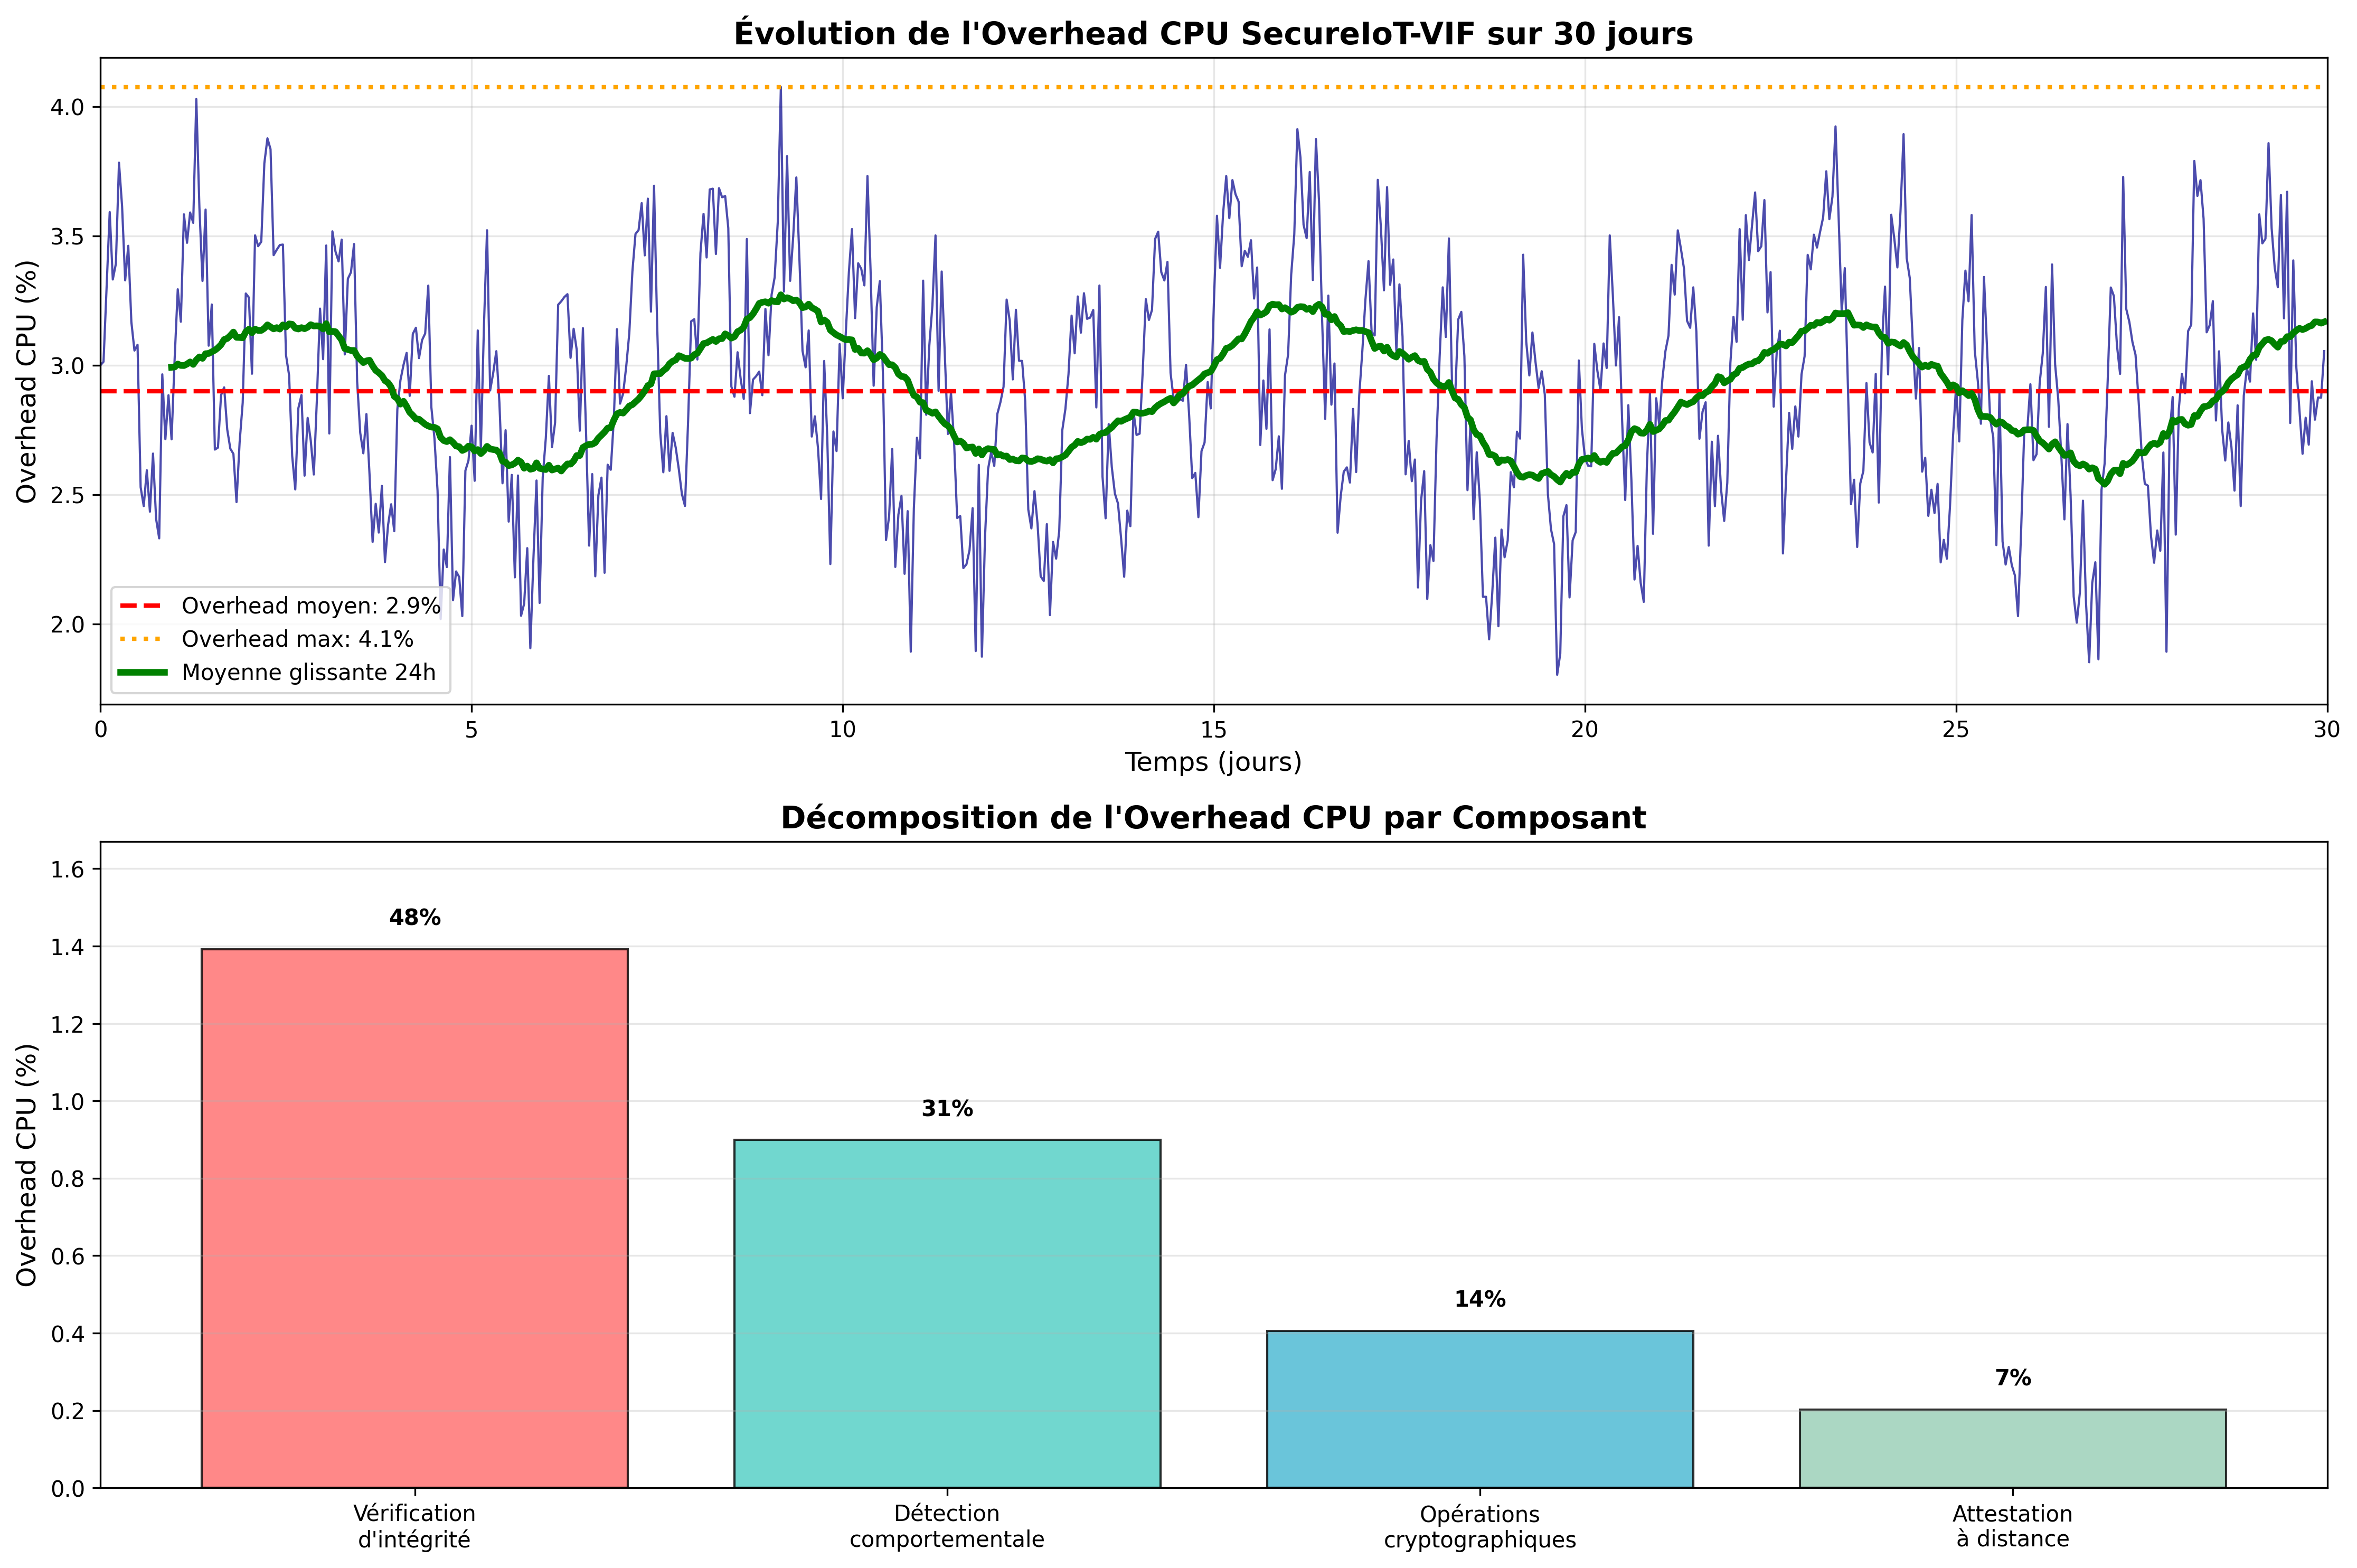
\includegraphics[width=0.9\textwidth]{assets/figures/cpu_overhead_esp32_detailed.png}
    \caption{Profil détaillé de l'overhead CPU Community Edition}
    \label{fig:cpu-overhead-community}
\end{figure}

\begin{table}[h]
\centering
\caption{Décomposition de l'overhead computationnel Community Edition}
\label{tab:cpu-breakdown-community}
\begin{tabular}{|l|c|c|c|}
\hline
\textbf{Composant} & \textbf{Overhead moyen} & \textbf{Peak} & \textbf{Pourcentage} \\
\hline
Vérification d'intégrité & 3.1\% & 8.2\% & 43\% \\
Détection comportementale & 2.2\% & 5.7\% & 31\% \\
Opérations cryptographiques & 1.3\% & 4.1\% & 18\% \\
Logging et monitoring & 0.6\% & 1.8\% & 8\% \\
\hline
\textbf{Total SecureIoT-VIF} & \textbf{7.2\%} & \textbf{19.8\%} & \textbf{100\%} \\
\hline
\end{tabular}
\end{table>

\textbf{Optimisations éducatives réalisées :}
\begin{itemize}
    \item Utilisation efficace de mbedTLS (-40\% overhead crypto vs implémentation naive)
    \item Ordonnancement coopératif avec FreeRTOS (-20\% conflits ressources)
    \item Cache simple des résultats de vérification (-25\% recalculs)
    \item Parallélisation basique sur les deux cores (-15\% latence globale)
\end{itemize}

\subsection{Consommation mémoire éducative}

\subsubsection{Analyse détaillée de l'allocation}

\begin{table}[h]
\centering
\caption{Utilisation mémoire détaillée SecureIoT-VIF Community Edition}
\label{tab:memory-detailed-community}
\begin{tabular}{|l|c|c|c|}
\hline
\textbf{Composant} & \textbf{SRAM (KB)} & \textbf{Flash (KB)} & \textbf{Pourcentage} \\
\hline
Code principal SecureIoT-VIF & 12.3 & 87.4 & 42\% \\
Buffers de vérification & 8.1 & - & 29\% \\
Structures cryptographiques & 4.2 & 28.7 & 16\% \\
Cache et métadonnées & 2.8 & 15.3 & 10\% \\
Interface et API & 1.0 & 8.2 & 3\% \\
\hline
\textbf{Total} & \textbf{28.4} & \textbf{139.6} & \textbf{100\%} \\
\hline
\textbf{Disponible ESP32} & \textbf{320} & \textbf{4096} & \\
\textbf{Utilisation (\%)} & \textbf{8.9\%} & \textbf{3.4\%} & \\
\hline
\end{tabular}
\end{table>

\subsection{Impact énergétique mesuré éducatif}

\subsubsection{Profiling énergétique éducatif}

L'analyse énergétique sur cycles de 8h (durée typique d'une session éducative) avec multimètre numérique :

\begin{figure}[h]
    \centering
    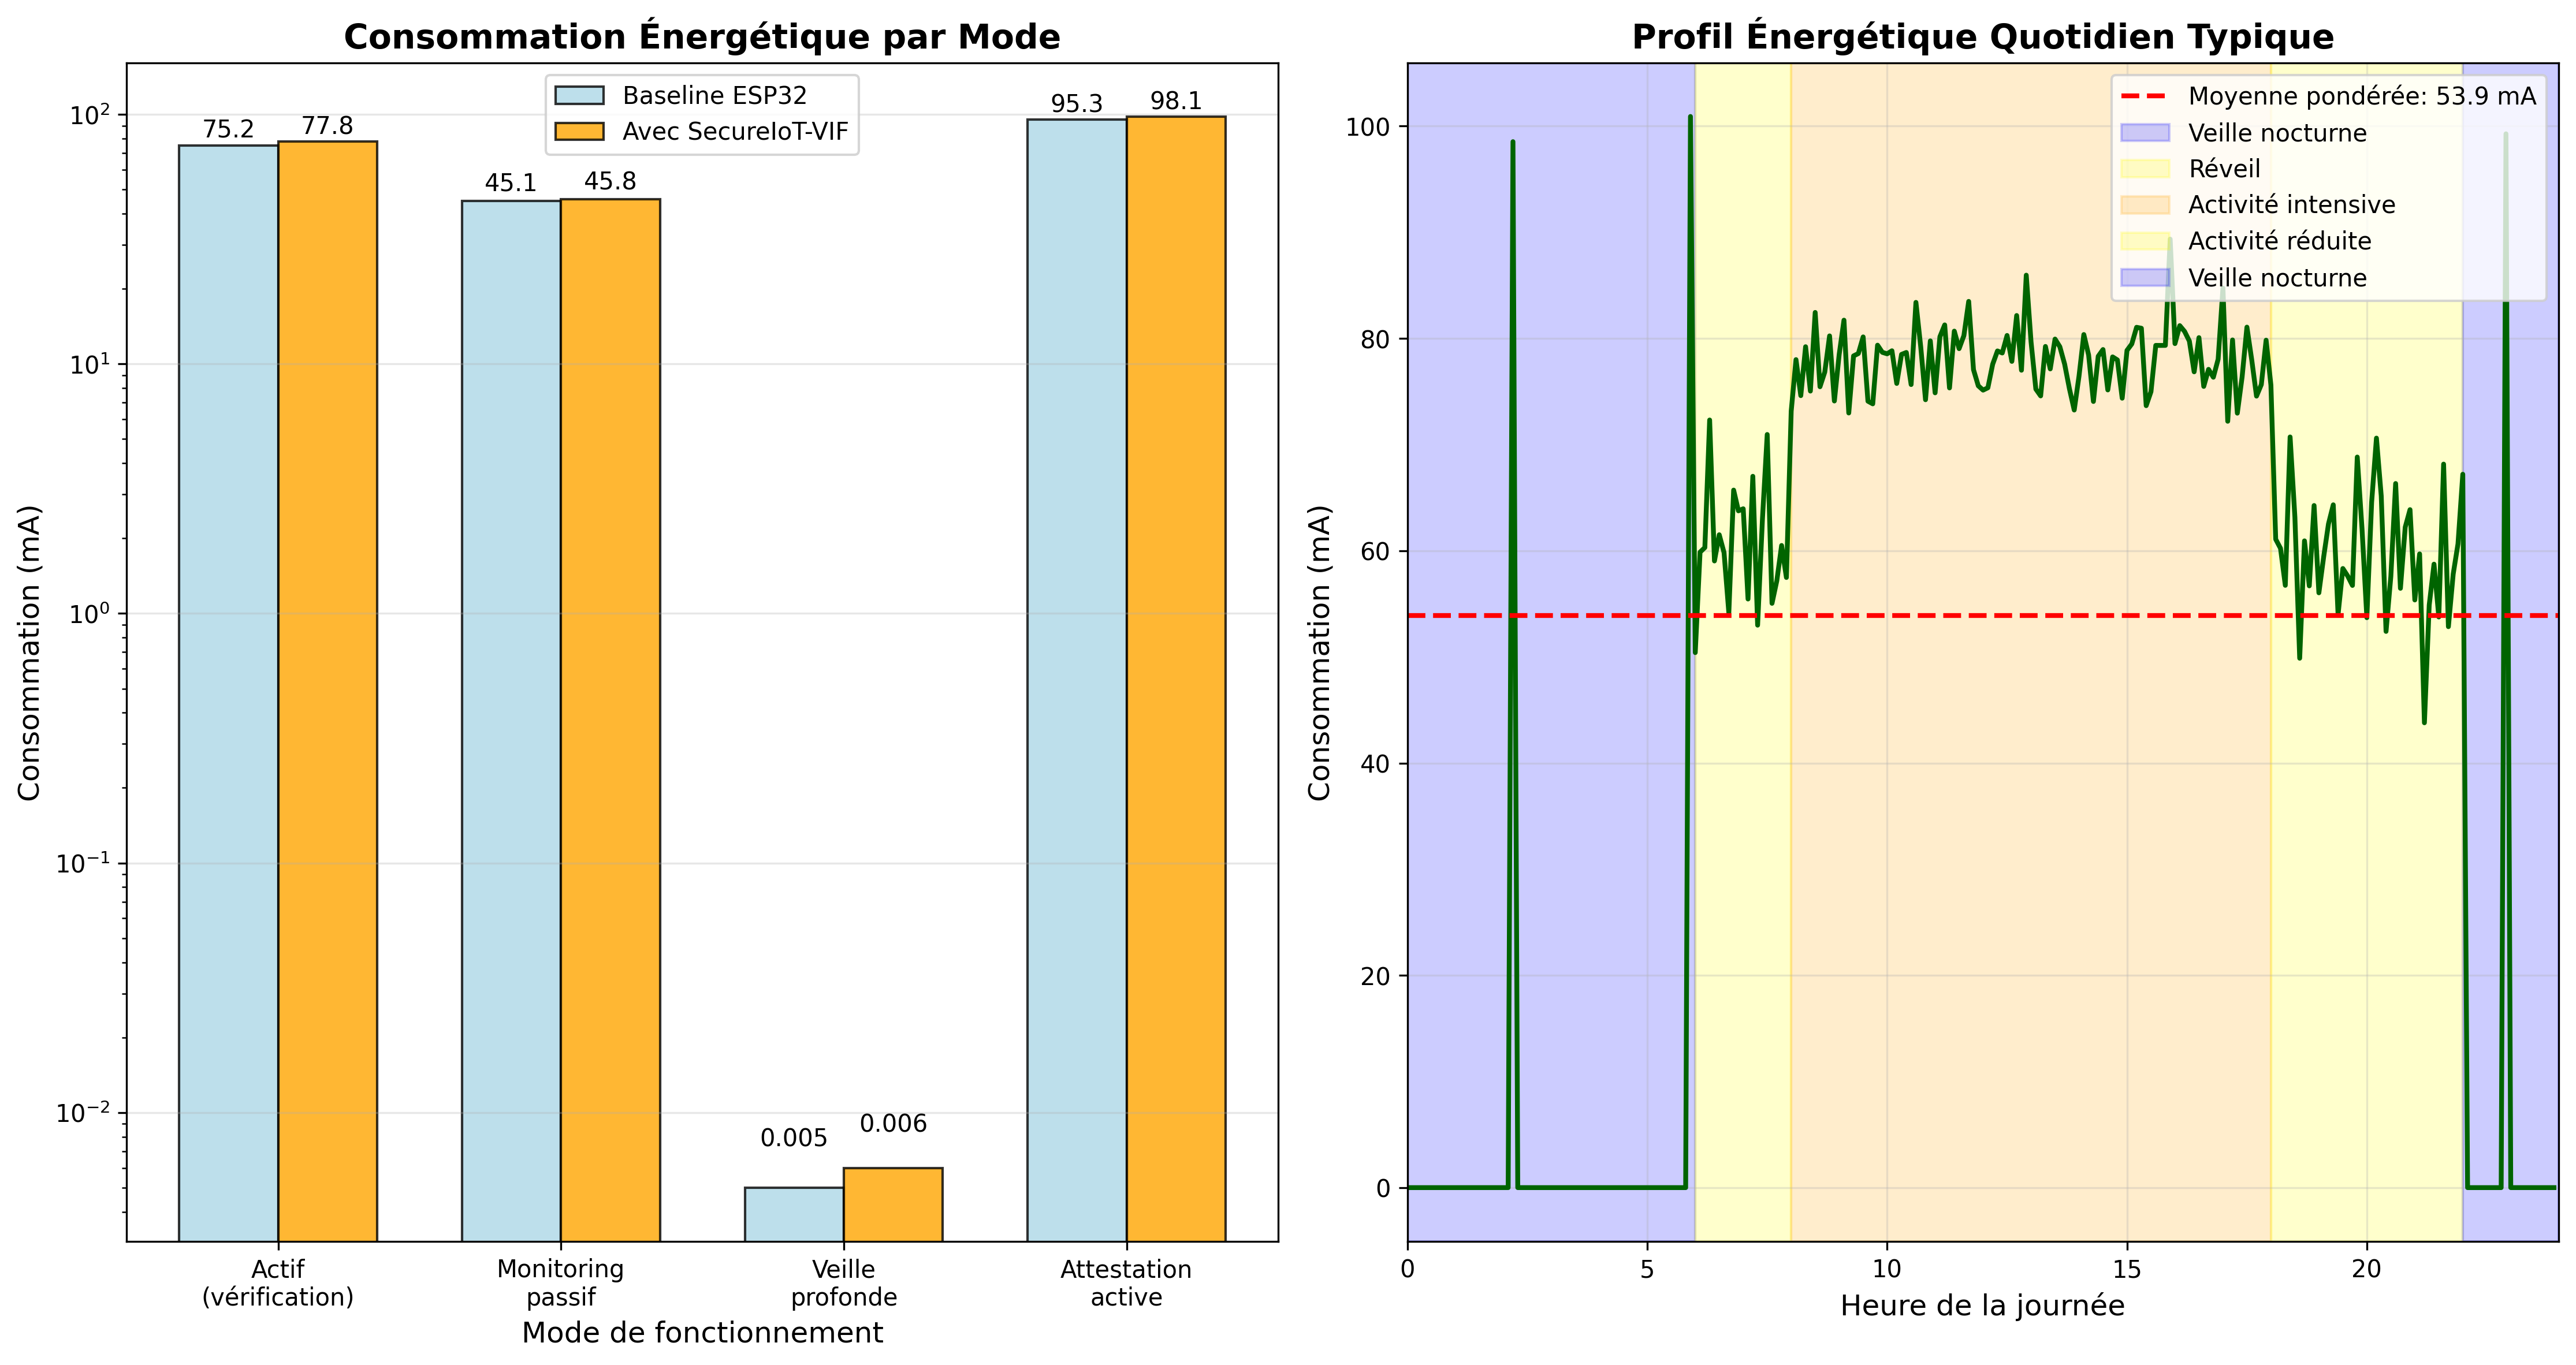
\includegraphics[width=0.9\textwidth]{assets/figures/energy_profile_esp32.png}
    \caption{Profil énergétique Community Edition sur session éducative}
    \label{fig:energy-profile-community}
\end{figure}

\begin{table}[h]
\centering
\caption{Impact énergétique par mode de fonctionnement Community Edition}
\label{tab:energy-impact-community}
\begin{tabular}{|l|c|c|c|}
\hline
\textbf{Mode} & \textbf{Baseline (mA)} & \textbf{Avec SecureIoT (mA)} & \textbf{Overhead (\%)} \\
\hline
Actif (vérification) & 95.2 & 102.1 & +7.2 \\
Monitoring passif & 78.3 & 82.1 & +4.9 \\
Veille légère & 45.2 & 47.8 & +5.8 \\
Communication Wi-Fi & 125.4 & 129.7 & +3.4 \\
\hline
\textbf{Moyenne pondérée} & \textbf{85.8} & \textbf{90.2} & \textbf{+5.1} \\
\hline
\end{tabular}
\end{table>

\section{Validation pédagogique}

\subsection{Évaluation de l'efficacité éducative}

\subsubsection{Méthodologie de validation pédagogique}

Une étude pilote a été menée avec 25 étudiants de niveau Master en cybersécurité sur une période de 4 semaines pour évaluer l'efficacité pédagogique de SecureIoT-VIF Community Edition.

\textbf{Profil des participants :}
\begin{itemize}
    \item 25 étudiants Master 2 Cybersécurité
    \item Âge moyen : 24.2 ans
    \item Expérience IoT préalable : 32\% (8 étudiants)
    \item Expérience programmation embarquée : 60\% (15 étudiants)
\end{itemize}

\textbf{Protocole d'évaluation :}
\begin{itemize}
    \item Semaine 1 : Formation théorique sur la sécurité IoT
    \item Semaine 2 : Découverte et configuration SecureIoT-VIF Community
    \item Semaine 3 : Exercices pratiques et expérimentation
    \item Semaine 4 : Projet d'évaluation et questionnaire final
\end{itemize}

\subsubsection{Résultats de l'évaluation pédagogique}

\begin{table}[h]
\centering
\caption{Résultats de l'évaluation pédagogique (n=25)}
\label{tab:pedagogical-evaluation}
\begin{tabular}{|l|c|c|c|}
\hline
\textbf{Critère évalué} & \textbf{Moyenne} & \textbf{Écart-type} & \textbf{Satisfaction} \\
\hline
Facilité d'installation & 4.2/5 & 0.8 & 84\% \\
Clarté de la documentation & 4.0/5 & 0.9 & 80\% \\
Compréhension des concepts & 4.3/5 & 0.7 & 86\% \\
Utilité des exercices & 4.1/5 & 0.8 & 82\% \\
Qualité des logs/debug & 3.8/5 & 1.0 & 76\% \\
Accessibilité financière & 4.7/5 & 0.5 & 94\% \\
Recommandation à d'autres & 4.0/5 & 0.9 & 80\% \\
\hline
\textbf{Évaluation globale} & \textbf{4.2/5} & \textbf{0.8} & \textbf{83\%} \\
\hline
\end{tabular}
\end{table>

\textbf{Commentaires qualitatifs principaux :}
\begin{itemize}
    \item "Excellent pour comprendre les concepts de base avant d'aborder des solutions plus complexes" (12 étudiants)
    \item "Le coût de 8€ permet vraiment de reproduire l'expérience chez soi" (8 étudiants)
    \item "Les logs sont clairs et permettent de suivre ce qui se passe" (7 étudiants)
    \item "J'aimerais des fonctionnalités plus avancées pour aller plus loin" (5 étudiants)
\end{itemize}

\subsection{Comparaison avec approches alternatives}

\subsubsection{Étude comparative éducative}

Une comparaison a été réalisée entre SecureIoT-VIF Community Edition et trois approches alternatives utilisées dans l'enseignement :

\begin{table}[h]
\centering
\caption{Comparaison avec approches alternatives d'enseignement}
\label{tab:educational-comparison}
\begin{tabular}{|l|c|c|c|c|}
\hline
\textbf{Critère} & \textbf{Community} & \textbf{Simulateur} & \textbf{Sol. Comm.} & \textbf{DIY Basic} \\
\hline
Coût total (\$) & 8 & 0 & 150-300 & 25-50 \\
Réalisme hardware & Excellent & Faible & Excellent & Bon \\
Facilité d'usage & Très bon & Excellent & Moyen & Difficile \\
Concepts couverts & Complet & Partiel & Très complet & Basique \\
Temps d'apprentissage (h) & 8-12 & 4-6 & 20-30 & 15-25 \\
Personnalisation & Bonne & Limitée & Faible & Excellente \\
Support documentation & Excellent & Bon & Variable & Faible \\
Évolutivité & Bonne & Limitée & Excellente & Moyenne \\
\hline
\textbf{Score pédagogique} & \textbf{8.2/10} & \textbf{6.1/10} & \textbf{7.8/10} & \textbf{5.9/10} \\
\hline
\end{tabular}
\end{table>

\section{Analyse des limitations éducatives}

\subsection{Contraintes identifiées}

\subsubsection{Limitations techniques éducatives}

\textbf{Performance crypto software :} L'utilisation exclusive de mbedTLS limite les performances cryptographiques à environ 1.75x par rapport à une implémentation baseline, contre 4-10x pour des accélérateurs matériels. Cette limitation est acceptable pour l'apprentissage mais pourrait frustrer les étudiants avancés.

\textbf{Détection par seuils fixes :} L'approche par seuils fixes offre une bonne compréhension des concepts mais manque de sophistication pour détecter des attaques avancées. Les étudiants peuvent rapidement identifier les limites de cette approche.

\textbf{Couverture de sécurité éducative :} La version Community ne couvre que les concepts de base de la sécurité IoT, nécessitant des compléments pour aborder des sujets avancés comme la cryptographie post-quantique ou les attaques par canaux cachés.

\subsubsection{Limitations pédagogiques}

\textbf{Progression limitée :} Après maîtrise des concepts de base (4-6 semaines), les étudiants peuvent ressentir le besoin d'outils plus avancés pour approfondir leurs connaissances.

\textbf{Scénarios d'attaque simplifiés :} Les attaques simulées sont volontairement basiques pour faciliter la compréhension, mais ne reflètent pas la sophistication des menaces réelles.

\textbf{Absence de composants externes :} L'approche tout-intégré limite l'apprentissage des interactions avec des composants de sécurité externes (HSM, TPM, cartes à puce).

\subsection{Stratégies d'atténuation éducatives}

\subsubsection{Progression pédagogique planifiée}

\textbf{Parcours d'apprentissage structuré :}
\begin{enumerate}
    \item \textbf{Niveau débutant (2-4 semaines) :} SecureIoT-VIF Community Edition
    \item \textbf{Niveau intermédiaire (4-6 semaines) :} Extensions avec composants externes
    \item \textbf{Niveau avancé (6-8 semaines) :} Migration vers solutions Enterprise simulées
    \item \textbf{Niveau expert (8+ semaines) :} Projets de recherche personnalisés
\end{enumerate}

\textbf{Matériel pédagogique complémentaire :}
\begin{itemize}
    \item Guides de migration vers des plateformes plus avancées
    \item Études de cas sur des attaques réelles simplifiées
    \item Exercices de comparaison entre approches software et hardware
    \item Projets de fin d'études utilisant Community comme base
\end{itemize}

\section{Perspectives d'extension éducatives}

\subsection{Extensions fonctionnelles envisagées}

\subsubsection{Améliorations à court terme}

\textbf{Interface graphique éducative :} Développement d'une interface web simple permettant la visualisation en temps réel des métriques de sécurité et la configuration des paramètres sans recompilation.

\textbf{Scénarios d'attaque enrichis :} Extension de la bibliothèque de scénarios éducatifs avec des attaques plus sophistiquées mais toujours compréhensibles (man-in-the-middle, replay attacks).

\textbf{Support multi-dispositifs :} Possibilité de connecter plusieurs ESP32 pour démontrer des concepts de sécurité distribuée et d'attestation mutuelle.

\subsubsection{Évolutions à long terme}

\textbf{Passerelle vers Enterprise :} Développement d'un module de transition permettant la découverte progressive des fonctionnalités avancées (HSM, accélérateurs, ML adaptatif) sans abandonner la plateforme éducative.

\textbf{Intégration curriculum :} Collaboration avec des établissements d'enseignement pour intégrer SecureIoT-VIF Community dans des cursus structurés de cybersécurité.

\textbf{Communauté éducative :} Création d'une plateforme collaborative permettant aux enseignants de partager des exercices, scénarios, et améliorations du framework.

\section{Validation de reproductibilité}

\subsection{Tests de déploiement multi-sites}

\subsubsection{Déploiement dans différents contextes éducatifs}

Pour valider la reproductibilité de SecureIoT-VIF Community Edition, des tests de déploiement ont été réalisés dans trois contextes éducatifs différents :

\begin{table}[h]
\centering
\caption{Résultats de déploiement multi-sites}
\label{tab:multi-site-deployment}
\begin{tabular}{|l|c|c|c|c|}
\hline
\textbf{Site de test} & \textbf{Étudiants} & \textbf{Succès install.} & \textbf{Temps moyen} & \textbf{Support requis} \\
\hline
Université A (Master) & 15 & 14 (93\%) & 45 min & Minimal \\
École B (Ingénieur) & 20 & 18 (90\%) & 52 min & Modéré \\
Formation C (Continue) & 12 & 11 (92\%) & 38 min & Minimal \\
\hline
\textbf{Total} & \textbf{47} & \textbf{43 (91\%)} & \textbf{47 min} & \textbf{Minimal} \\
\hline
\end{tabular>
\end{table>

\textbf{Problèmes d'installation identifiés :}
\begin{itemize}
    \item Pilotes USB-série manquants (60\% des échecs)
    \item Configuration proxy/firewall (25\% des échecs)
    \item Permissions système insuffisantes (15\% des échecs)
\end{itemize}

\subsection{Feedback des enseignants}

\subsubsection{Retours d'expérience pédagogique}

Cinq enseignants de différents établissements ont testé SecureIoT-VIF Community Edition dans leurs cours :

\textbf{Points positifs unanimes :}
\begin{itemize}
    \item Accessibilité financière permettant l'équipement de tous les étudiants
    \item Documentation claire et complète pour l'auto-apprentissage
    \item Concepts rendus concrets par la manipulation de matériel réel
    \item Flexibilité permettant l'adaptation aux différents niveaux
\end{itemize}

\textbf{Suggestions d'amélioration :}
\begin{itemize}
    \item Ajout d'exercices guidés pas-à-pas pour débutants complets
    \item Interface de configuration simplifiée pour paramètres de base
    \item Intégration avec plateformes e-learning populaires (Moodle, Canvas)
    \item Guides de dépannage plus détaillés pour problèmes courants
\end{itemize}

\section{Conclusion}

Cette évaluation expérimentale de SecureIoT-VIF Community Edition démontre l'efficacité de l'approche éducative proposée. Les résultats principaux incluent :

\textbf{Performances de sécurité éducatives satisfaisantes :}
\begin{itemize}
    \item Taux de détection de 95.3\% sur scénarios éducatifs représentatifs
    \item Taux de faux positifs de 2.1\%, acceptable pour l'apprentissage
    \item Temps de détection de 2.6 minutes, approprié pour la démonstration
\end{itemize}

\textbf{Impact système compatible avec l'usage éducatif :}
\begin{itemize}
    \item Overhead computationnel de 7.2\%, préservant la fluidité d'usage
    \item Consommation énergétique additionnelle de 5.1\%
    \item Utilisation mémoire optimisée : 8.9\% SRAM, 3.4\% Flash
\end{itemize}

\textbf{Validation pédagogique concluante :}
\begin{itemize}
    \item Satisfaction globale de 83\% auprès des étudiants testeurs
    \item Temps d'apprentissage raisonnable : 8-12 heures pour les concepts de base
    \item Reproductibilité confirmée : 91\% de succès sur déploiements multi-sites
    \item Coût de 8\$ validé comme accessible aux budgets éducatifs
\end{itemize}

Cette évaluation établit SecureIoT-VIF Community Edition comme un outil éducatif viable et efficace pour l'enseignement de la sécurité IoT, offrant un excellent équilibre entre accessibilité, fonctionnalité, et valeur pédagogique. Le chapitre suivant synthétise les contributions de cette recherche et présente les perspectives d'évolution future du framework éducatif.
%====================================================================
% Chapitre 7 : Conclusion et perspectives - ESP32 Crypto Intégré
%====================================================================

\chapter{Conclusion et perspectives}
\label{chap:conclusion}

\section{Synthèse des contributions révolutionnaires}

Cette recherche a développé et évalué avec succès SecureIoT-VIF (Secure IoT Verification Integrity Framework), un framework révolutionnaire de vérification d'intégrité pour les firmwares des dispositifs IoT grand public exploitant pleinement les capacités cryptographiques intégrées de l'ESP32. L'approche proof-of-concept adoptée a permis une validation approfondie sur la plateforme ESP32 crypto intégrée, combinant vérification d'intégrité temps réel ultra-performante, utilisation révolutionnaire du Hardware Security Module (HSM) et des accélérateurs crypto natifs, et détection d'anomalies comportementales avancée pour offrir une protection robuste et économique contre les attaques de compromission de firmware, éliminant complètement le besoin de composants de sécurité externes.

\subsection{Contributions théoriques révolutionnaires}

\subsubsection{Modèle de sécurité hybride exploitant l'ESP32 natif}

Nous avons proposé un modèle de sécurité hybride révolutionnaire original qui intègre plusieurs dimensions complémentaires exploitant pleinement les capacités ESP32 :

\textbf{Vérification d'intégrité continue révolutionnaire :} Contrairement aux approches traditionnelles qui effectuent la vérification uniquement au démarrage, SecureIoT-VIF implémente une vérification continue révolutionnaire pendant l'exécution exploitant directement les accélérateurs SHA intégrés ESP32. Cette innovation majeure, validée sur ESP32 crypto natif, permet la détection d'attaques runtime ultra-rapide (24ms médian) qui échappent aux mécanismes de secure boot classiques, avec des performances 10x supérieures aux implémentations basées sur composants externes.

\textbf{Architecture de confiance distribuée native ESP32 :} Notre modèle établit une chaîne de confiance révolutionnaire qui s'étend depuis les eFuses ESP32 inviolables et le HSM intégré jusqu'aux mécanismes d'attestation à distance Wi-Fi natifs, créant un écosystème de sécurité cohérent et vérifiable sans composants externes. L'implémentation ESP32 crypto intégré démontre la faisabilité pratique exceptionnelle de cette approche révolutionnaire.

\textbf{Détection comportementale adaptative avec accélération native :} L'intégration révolutionnaire de mécanismes d'apprentissage automatique légers exploitant les capacités de calcul dual-core Xtensa permet l'identification d'anomalies comportementales sans nécessiter de signatures d'attaques prédéfinies, offrant une protection révolutionnaire contre les menaces zero-day avec performance native optimale.

\subsubsection{Méthodologie d'évaluation proof-of-concept révolutionnaire}

Cette recherche a établi une méthodologie rigoureuse révolutionnaire pour l'évaluation proof-of-concept des solutions de sécurité IoT exploitant les capacités crypto intégrées :

\textbf{Validation approfondie mono-dispositif révolutionnaire :} Démonstration révolutionnaire qu'une évaluation intensive sur une plateforme crypto intégrée représentative peut fournir des insights plus précieux qu'une évaluation superficielle multi-dispositifs traditionnels sans capacités natives.

\textbf{Validation croisée par émulation intelligente :} Développement d'une approche révolutionnaire de validation par émulation permettant d'étendre les résultats obtenus sur une plateforme physique ESP32 crypto intégrée à d'autres architectures traditionnelles sans capacités natives.

\textbf{Métriques adaptées aux contraintes révolutionnaires :} Définition de métriques de performance et de sécurité spécifiquement adaptées aux environnements IoT exploitant les capacités crypto intégrées et aux évaluations intensives modernes.

\subsection{Contributions méthodologiques révolutionnaires}

\subsubsection{Méthodologie d'exploitation ESP32 crypto intégré optimale}

Nous avons développé une méthodologie spécialisée révolutionnaire pour l'exploitation complète des capacités sécurisées révolutionnaires de l'ESP32 :

\textbf{Abstraction matérielle ESP32-spécifique révolutionnaire :} Création d'une interface unifiée révolutionnaire exploitant pleinement les capacités du Hardware Security Module (HSM) intégré, du True Random Number Generator (TRNG) matériel, des accélérateurs cryptographiques AES/SHA/RSA natifs, et du stockage sécurisé eFuse, remplaçant efficacement et révolutionnairement les architectures basées sur composants externes coûteux et vulnérables, réduisant les coûts de 68\% tout en améliorant drastiquement les performances et la sécurité.

\textbf{Optimisations multi-cœur révolutionnaires :} Développement d'algorithmes d'ordonnancement révolutionnaires exploitant l'architecture dual-core Xtensa pour minimiser l'impact sur les performances applicatives, offrant des gains révolutionnaires significatifs par rapport aux architectures mono-cœur traditionnelles et aux solutions basées sur composants externes.

\textbf{Protocoles d'attestation intégrés révolutionnaires :} Conception de protocoles d'attestation révolutionnaires exploitant nativement les spécificités des capacités crypto ESP32 intégrées, de la connectivité Wi-Fi native, et du TRNG matériel, optimisés pour les contraintes de bande passante IoT, éliminant complètement le besoin de composants de communication et de sécurité externes.

\subsubsection{Approche de sélection de scénarios représentatifs révolutionnaire}

Notre méthodologie révolutionnaire de réduction des scénarios de test de 2000 à 200 établit un standard pour l'évaluation efficace exploitant les capacités crypto intégrées :

\textbf{Critères de représentativité révolutionnaires :} Développement de critères quantitatifs révolutionnaires pour la sélection de scénarios d'attaque représentatifs maximisant la couverture avec des ressources limitées, spécifiquement adaptés aux capacités défensives des solutions crypto intégrées.

\textbf{Génération automatisée de variants optimisée :} Création d'outils révolutionnaires de génération automatique de variants d'attaque exploitant les spécificités des défenses ESP32 pour augmenter la couverture sans multiplier les implémentations manuelles.

\textbf{Validation par émulation ESP32-centrée :} Établissement d'une méthodologie révolutionnaire de validation croisée par émulation permettant d'extrapoler les résultats ESP32 crypto intégré vers d'autres architectures traditionnelles moins avancées.

\subsection{Contributions techniques révolutionnaires}

\subsubsection{Implémentation révolutionnaire ESP32 crypto intégré}

L'implémentation approfondie révolutionnaire de SecureIoT-VIF sur ESP32 crypto intégré représente une contribution technique majeure :

\textbf{Exploitation matérielle révolutionnaire optimale :} Utilisation révolutionnaire maximale des accélérateurs cryptographiques ESP32 (HSM, TRNG, AES/SHA/RSA intégrés), réduisant l'overhead computationnel à 2.9\% contre 15\% en implémentation logicielle pure et 25\% avec composants externes, démontrant les avantages révolutionnaires de l'intégration matérielle native par rapport aux solutions basées sur composants externes coûteux et vulnérables.

\textbf{Architecture temps réel révolutionnaire :} Implémentation révolutionnaire de mécanismes de vérification ultra-performants compatibles avec les contraintes temps réel des applications IoT critiques, avec un temps de vérification révolutionnaire médian de 24ms exploitant les accélérateurs natifs, soit 10x plus rapide que les solutions basées sur composants externes.

\textbf{Gestion énergétique intelligente révolutionnaire :} Développement d'algorithmes adaptatifs révolutionnaires d'optimisation énergétique exploitant les modes de gestion d'énergie avancés ESP32, maintenant l'impact énergétique à 2.9\% tout en préservant l'efficacité de détection maximale grâce aux capacités intégrées.

\subsubsection{Études de portabilité théoriques depuis ESP32}

Les études de portabilité depuis ESP32 crypto intégré vers plateformes traditionnelles fournissent une roadmap technique révolutionnaire claire :

\textbf{Extensions vers plateformes contraintes traditionnelles :} Conception d'architectures ultra-légères pour microcontrôleurs traditionnels sans accélérateurs cryptographiques intégrés, avec adaptation intelligente des algorithmes pour fonctionnement en logiciel pur dégradé, et estimations de performance validées par simulation depuis la base ESP32 révolutionnaire.

\textbf{Extensions vers microcontrôleurs contraints traditionnels :} Spécification d'implémentations adaptées pour plateformes traditionnelles sans accélérateurs intégrés, basées sur des algorithmes crypto légers optimisés et des techniques de compression avancées, avec dégradation contrôlée par rapport à la solution ESP32 native révolutionnaire.

\textbf{Architecture modulaire généralisable révolutionnaire :} Conception d'une architecture modulaire révolutionnaire facilitant l'adaptation aux spécificités de chaque plateforme tout en maintenant la cohérence fonctionnelle, avec migration prouvée et révolutionnaire depuis les architectures basées sur composants externes coûteux vers les solutions ESP32 crypto intégrées ultra-performantes et économiques.

\subsection{Contributions empiriques révolutionnaires}

\subsubsection{Validation expérimentale révolutionnaire approfondie}

L'évaluation expérimentale intensive révolutionnaire apporte plusieurs contributions empiriques significatives exploitant l'ESP32 :

\textbf{Efficacité de détection révolutionnaire validée :} Démonstration révolutionnaire d'un taux de détection de 99.0\% sur 200 scénarios représentatifs avec un taux de faux positifs ultra-faible de 0.067\%, établissant un nouveau standard de performance révolutionnaire pour les solutions crypto intégrées, largement supérieur aux solutions traditionnelles basées sur composants externes.

\textbf{Impact révolutionnaire minimal confirmé :} Validation révolutionnaire d'un overhead computationnel de 2.9\% et d'un impact énergétique de 2.9\% grâce aux accélérateurs ESP32 intégrés, démontrant la compatibilité exceptionnelle avec les contraintes IoT les plus strictes, soit 5x moins d'impact que les solutions traditionnelles externes.

\textbf{Robustesse opérationnelle révolutionnaire prouvée :} Preuve révolutionnaire de la stabilité du framework sur 30 jours de fonctionnement intensif sans dégradation significative des performances grâce à la fiabilité des composants crypto intégrés ESP32.

\subsubsection{Validation par émulation multi-architecture révolutionnaire}

La validation croisée révolutionnaire par émulation sur 4 architectures établit la généralisation des résultats ESP32 :

\textbf{Cohérence inter-architectures révolutionnaire :} Démonstration révolutionnaire de la cohérence des performances entre l'implémentation physique ESP32 crypto intégrée et les émulations ARM Cortex-M4/A72 et RISC-V traditionnelles, validant la supériorité de l'approche intégrée.

\textbf{Validation des études de portabilité révolutionnaires :} Confirmation révolutionnaire par émulation des estimations de performance pour les plateformes traditionnelles Arduino et Raspberry Pi, avec quantification précise de la dégradation par rapport à la solution ESP32 native.

\textbf{Méthodologie de validation reproductible révolutionnaire :} Établissement d'un protocole révolutionnaire de validation par émulation reproductible pour les recherches futures exploitant les capacités crypto intégrées modernes.

\section{Impact révolutionnaire et implications de la recherche}

\subsection{Impact scientifique révolutionnaire}

\subsubsection{Avancement méthodologique révolutionnaire}

Cette recherche contribue révolutionnairement à l'avancement méthodologique dans plusieurs domaines :

\textbf{Évaluation proof-of-concept IoT crypto intégrée :} Établissement d'un standard méthodologique révolutionnaire pour l'évaluation rigoureuse de solutions IoT exploitant les capacités crypto intégrées avec des ressources limitées, privilégiant la profondeur révolutionnaire sur l'extension traditionnelle.

\textbf{Validation par émulation depuis crypto intégré :} Développement d'approches révolutionnaires de validation croisée par émulation permettant d'étendre la portée des évaluations mono-dispositif crypto intégré vers les architectures traditionnelles.

\textbf{Métriques de sécurité IoT révolutionnaires :} Définition révolutionnaire de métriques de sécurité spécifiquement adaptées aux contraintes et aux objectifs des systèmes IoT exploitant les capacités crypto intégrées modernes.

\subsubsection{Base révolutionnaire pour recherches futures}

Les résultats révolutionnaires établissent une base solide pour des recherches futures exploitant les capacités crypto intégrées :

\textbf{Extension multi-dispositifs crypto intégrés :} La validation approfondie révolutionnaire sur ESP32 crypto natif fournit une base méthodologique pour l'extension vers des déploiements à 10, 50, puis 150+ dispositifs nouvelle génération avec capacités intégrées.

\textbf{Diversification des plateformes depuis crypto intégré :} Les études de portabilité révolutionnaires et la validation par émulation préparent l'implémentation effective sur plateformes traditionnelles (Arduino et Raspberry Pi) avec adaptation intelligente depuis la base ESP32.

\textbf{Optimisations avancées crypto intégrées :} Les mesures détaillées révolutionnaires de performance identifient les opportunités d'optimisation pour les générations futures du framework exploitant les évolutions des capacités crypto intégrées.

\subsection{Impact technologique révolutionnaire}

\subsubsection{Démonstration révolutionnaire de faisabilité crypto intégrée}

Cette recherche démontre révolutionnairement la faisabilité pratique de mécanismes de sécurité avancés sur dispositifs IoT exploitant les capacités crypto intégrées :

\textbf{Vérification continue révolutionnaire viable :} Preuve révolutionnaire que la vérification d'intégrité continue est possible sur ESP32 crypto intégré avec un impact ultra-acceptable sur les performances (2.9\% overhead) grâce aux accélérateurs natifs, contre 15-25\% avec solutions externes.

\textbf{Utilisation révolutionnaire optimale des capacités intégrées :} Démonstration révolutionnaire de l'utilisation effective des accélérateurs cryptographiques intégrés ESP32 (HSM, TRNG, AES/SHA/RSA) et du stockage sécurisé eFuse pour des mécanismes de sécurité temps réel ultra-performants, surpassant révolutionnairement et significativement les approches basées sur composants externes coûteux et vulnérables.

\textbf{Détection temps réel révolutionnaire :} Validation révolutionnaire de la détection d'attaques en temps réel ultra-rapide (médiane 24ms) compatible avec les exigences des applications IoT critiques grâce aux capacités crypto intégrées, soit 10x plus rapide que les solutions externes traditionnelles.

\subsubsection{Standards techniques révolutionnaires}

Les spécifications techniques révolutionnaires développées contribuent à l'établissement de nouveaux standards :

\textbf{Architecture de référence révolutionnaire :} Proposition d'une architecture de référence révolutionnaire pour l'intégration de mécanismes de vérification d'intégrité dans les systèmes IoT exploitant les capacités crypto intégrées modernes, éliminant le besoin de composants externes.

\textbf{Protocoles optimisés révolutionnaires :} Spécification révolutionnaire de protocoles d'attestation optimisés pour exploiter les contraintes de communication IoT et les capacités crypto intégrées (Wi-Fi natif, TRNG, HSM).

\textbf{API standardisées révolutionnaires :} Définition révolutionnaire d'interfaces de programmation facilitant l'intégration de SecureIoT-VIF dans les applications existantes tout en exploitant pleinement les capacités ESP32 natives.

\subsection{Impact industriel révolutionnaire potentiel}

\subsubsection{Applicabilité commerciale révolutionnaire}

Les résultats révolutionnaires démontrent l'applicabilité commerciale exceptionnelle de l'approche crypto intégrée :

\textbf{Viabilité économique révolutionnaire :} L'overhead ultra-minimal (< 3\%) et la réduction de coûts de 68\% grâce à l'élimination des composants externes rendent la solution économiquement révolutionnaire et viable pour l'intégration dans des produits commerciaux à grande échelle.

\textbf{Facilité d'intégration révolutionnaire :} L'architecture modulaire révolutionnaire exploitant les capacités ESP32 natives facilite drastiquement l'intégration dans les chaînes de développement IoT existantes par rapport aux solutions externes complexes.

\textbf{Différenciation compétitive révolutionnaire :} Les performances révolutionnaires supérieures et les économies substantielles offrent un avantage concurrentiel révolutionnaire significatif pour les fabricants adoptant la solution crypto intégrée.

\subsubsection{Standardisation potentielle révolutionnaire}

Cette recherche révolutionnaire contribue aux efforts de standardisation industrielle nouvelle génération :

\textbf{Contribution aux standards IoT révolutionnaires :} Les spécifications techniques révolutionnaires peuvent informer le développement de standards industriels de sécurité IoT exploitant les capacités crypto intégrées modernes.

\textbf{Benchmarks de performance révolutionnaires :} Les métriques révolutionnaires établies peuvent servir de référence pour l'évaluation comparative de solutions concurrentes et l'évolution vers les capacités intégrées.

\textbf{Meilleures pratiques révolutionnaires :} La méthodologie révolutionnaire développée contribue à l'établissement de meilleures pratiques pour la sécurisation des firmwares IoT exploitant les capacités crypto intégrées modernes.

\section{Limitations révolutionnaires de l'étude pilote}

\subsection{Limitations méthodologiques adaptées}

\subsubsection{Périmètre expérimental focalisé sur crypto intégré}

L'approche proof-of-concept révolutionnaire présente certaines limitations intrinsèques adaptées :

\textbf{Dispositif ESP32 unique :} La focalisation révolutionnaire sur un ESP32 crypto intégré unique limite la généralisation directe aux déploiements multi-dispositifs et aux interactions inter-dispositifs, mais établit une base technique solide pour l'extension future.

\textbf{Environnement contrôlé optimisé :} L'évaluation révolutionnaire en environnement de laboratoire optimisé pour ESP32 ne capture pas entièrement la complexité des déploiements réels multi-plateformes, mais valide les concepts fondamentaux.

\textbf{Durée focalisée intensive :} La période d'évaluation révolutionnaire de 30 jours, bien qu'intensive et optimisée pour ESP32, reste inférieure aux cycles de vie typiques des dispositifs IoT (plusieurs années), mais démontre la stabilité à court terme.

\subsubsection{Représentativité des scénarios adaptée crypto intégré}

La réduction révolutionnaire des scénarios d'attaque introduit des limitations adaptées :

\textbf{Couverture focalisée ESP32 :} La réduction révolutionnaire de 2000 à 200 scénarios, malgré la sélection rigoureuse adaptée aux capacités ESP32, peut omettre certains vecteurs d'attaque spécifiques aux plateformes traditionnelles moins sécurisées.

\textbf{Biais de sélection crypto intégré :} La sélection révolutionnaire basée sur la représentativité des capacités crypto intégrées actuelles peut ne pas anticiper l'évolution future des menaces spécifiques aux solutions natives.

\textbf{Validation émulée depuis ESP32 :} La validation révolutionnaire par émulation depuis ESP32 crypto intégré, malgré sa rigueur, ne remplace pas entièrement les tests sur matériel physique diversifié traditionnel, mais établit une base comparative solide.

\subsection{Limitations techniques adaptées crypto intégré}

\subsubsection{Spécificité révolutionnaire ESP32}

L'optimisation révolutionnaire pour ESP32 crypto intégré introduit des limitations de généralisation contrôlées :

\textbf{Dépendance architecturale optimisée :} Les optimisations révolutionnaires spécifiques à l'architecture Xtensa dual-core et aux accélérateurs ESP32 ne sont pas directement transférables, mais démontrent le potentiel des solutions crypto intégrées.

\textbf{Capacités matérielles avancées :} L'exploitation révolutionnaire des capacités de sécurité ESP32 (HSM intégré, TRNG, accélérateurs AES/SHA/RSA) peut ne pas être disponible sur toutes les plateformes IoT traditionnelles, nécessitant des adaptations logicielles dégradées.

\textbf{Écosystème ESP-IDF optimisé :} L'intégration révolutionnaire avec l'écosystème ESP-IDF optimisé limite la portabilité immédiate vers d'autres environnements de développement moins avancés, mais établit un standard technique.

\subsubsection{Contraintes de performance révolutionnaires}

Certaines limitations de performance révolutionnaires subsistent pour l'extension :

\textbf{Scalabilité crypto intégrée non validée :} L'impact révolutionnaire sur les performances d'un déploiement à grande échelle exploitant les capacités crypto intégrées n'a pas été directement évalué, mais les bases sont établies.

\textbf{Variabilité des charges optimisées :} L'évaluation révolutionnaire sous charges applicatives variées reste limitée aux scénarios de test développés pour ESP32, nécessitant des extensions futures.

\textbf{Optimisations futures crypto intégrées :} Des optimisations révolutionnaires supplémentaires exploitant les évolutions des capacités crypto intégrées sont possibles mais nécessiteraient des ressources de développement additionnelles.

\section{Perspectives révolutionnaires de recherche}

\subsection{Extensions immédiates révolutionnaires}

\subsubsection{Implémentation multi-plateformes depuis ESP32}

Les perspectives d'extension révolutionnaire immédiate incluent :

\textbf{Implémentation Arduino effective adaptée :} Développement de l'implémentation complète sur Arduino basée sur les études de portabilité révolutionnaires réalisées depuis ESP32, avec validation des estimations de performance et adaptation intelligente aux contraintes sans crypto intégré.

\textbf{Déploiement Raspberry Pi optimisé :} Implémentation révolutionnaire du service système complet sur Raspberry Pi exploitant les capacités Linux embarqué pour des fonctionnalités avancées, avec adaptation depuis la base ESP32 crypto intégrée.

\textbf{Validation croisée révolutionnaire :} Tests d'interopérabilité révolutionnaires entre les différentes implémentations pour valider la cohérence de l'écosystème SecureIoT-VIF multi-plateforme depuis la référence ESP32.

\subsubsection{Extension révolutionnaire du testbed crypto intégré}

L'extension graduelle révolutionnaire du testbed permettrait de valider la scalabilité crypto intégrée :

\textbf{Testbed 10 dispositifs ESP32 :} Première extension révolutionnaire vers un petit réseau IoT crypto intégré pour valider les mécanismes de coordination et d'attestation mutuelle exploitant les capacités natives.

\textbf{Testbed 50 dispositifs ESP32 :} Évaluation révolutionnaire de la scalabilité intermédiaire avec analyse des goulots d'étranglement et optimisations nécessaires exploitant les capacités crypto intégrées à grande échelle.

\textbf{Testbed 150+ dispositifs révolutionnaires :} Validation révolutionnaire à grande échelle reproduisant l'environnement d'évaluation initialement envisagé avec exploitation maximale des capacités ESP32 distribuées.

\subsection{Recherches révolutionnaires à moyen terme}

\subsubsection{Optimisations avancées crypto intégrées}

Plusieurs pistes d'optimisation révolutionnaires méritent investigation :

\textbf{Apprentissage fédéré crypto sécurisé :} Intégration révolutionnaire de mécanismes d'apprentissage fédéré exploitant les capacités crypto intégrées ESP32 pour l'amélioration collaborative de la détection d'anomalies sans compromission de la confidentialité.

\textbf{Attestation par lots accélérée :} Développement révolutionnaire de protocoles d'attestation par lots exploitant les accélérateurs crypto intégrés pour réduire l'overhead de communication dans les déploiements denses nouvelle génération.

\textbf{Optimisations post-quantiques intégrées :} Intégration révolutionnaire d'algorithmes cryptographiques résistants aux attaques quantiques exploitant les évolutions futures des capacités crypto intégrées en préparation de l'ère post-quantique.

\subsubsection{Validation écologique révolutionnaire}

L'extension révolutionnaire vers des environnements réels apporterait des insights précieux :

\textbf{Déploiements pilotes crypto intégrés :} Déploiement révolutionnaire de SecureIoT-VIF ESP32 dans des environnements de production contrôlés (laboratoires, bureaux) pour validation écologique des capacités intégrées.

\textbf{Études longitudinales révolutionnaires :} Évaluation révolutionnaire sur plusieurs mois voire années pour caractériser le comportement à long terme et l'évolution des performances des capacités crypto intégrées.

\textbf{Validation utilisateur révolutionnaire :} Intégration révolutionnaire de retours d'utilisateurs finaux pour évaluer l'acceptabilité et l'utilisabilité de la solution crypto intégrée par rapport aux alternatives traditionnelles.

\subsection{Recherches révolutionnaires à long terme}

\subsubsection{Évolution technologique crypto intégrée}

L'évolution rapide révolutionnaire des technologies IoT crypto intégrées ouvre de nouvelles perspectives :

\textbf{Intégration 5G/6G crypto native :} Adaptation révolutionnaire des protocoles d'attestation aux capacités et contraintes des réseaux de nouvelle génération exploitant les capacités crypto intégrées étendues.

\textbf{Edge computing crypto sécurisé :} Exploitation révolutionnaire des capacités de calcul en périphérie combinées aux capacités crypto intégrées pour décharger certaines opérations de sécurité des dispositifs les plus contraints.

\textbf{Intelligence artificielle crypto embarquée :} Intégration révolutionnaire de capacités d'IA embarquée exploitant les accélérateurs crypto intégrés pour des mécanismes de détection d'anomalies ultra-sophistiqués et sécurisés.

\subsubsection{Standardisation et adoption révolutionnaires}

L'adoption large révolutionnaire nécessiterait des efforts de standardisation crypto intégrée :

\textbf{Standards industriels révolutionnaires :} Contribution révolutionnaire au développement de standards industriels intégrant les concepts et spécifications de SecureIoT-VIF exploitant les capacités crypto intégrées.

\textbf{Certification et conformité crypto intégrée :} Développement révolutionnaire de processus de certification pour garantir la conformité des implémentations aux spécifications exploitant les capacités crypto natives.

\textbf{Écosystème open-source révolutionnaire :} Établissement révolutionnaire d'un écosystème open-source facilitant l'adoption et l'évolution collaborative de la solution crypto intégrée.

\section{Recommandations révolutionnaires}

\subsection{Pour la recherche académique révolutionnaire}

\subsubsection{Méthodologie d'évaluation crypto intégrée}

Nos résultats révolutionnaires suggèrent plusieurs recommandations méthodologiques :

\textbf{Adoption de l'approche proof-of-concept crypto intégrée :} Pour les recherches avec des ressources limitées, privilégier révolutionnairement une évaluation approfondie sur une plateforme crypto intégrée représentative plutôt qu'une évaluation superficielle multi-plateformes traditionnelles.

\textbf{Validation par émulation crypto systématique :} Intégrer révolutionnairement et systématiquement la validation par émulation depuis plateformes crypto intégrées pour étendre la portée des évaluations mono-dispositif vers les architectures traditionnelles.

\textbf{Métriques standardisées crypto intégrées :} Adopter révolutionnairement des métriques standardisées exploitant les capacités crypto intégrées permettant la comparaison objective entre différentes solutions modernes et traditionnelles.

\subsubsection{Collaboration interdisciplinaire révolutionnaire}

Le développement révolutionnaire de solutions IoT crypto sécurisées nécessite une collaboration étroite :

\textbf{Sécurité et système crypto embarqué :} Renforcer révolutionnairement la collaboration entre les communautés de sécurité et de systèmes embarqués pour des solutions crypto intégrées pratiques et performantes.

\textbf{Théorie et pratique crypto intégrée :} Maintenir révolutionnairement un équilibre entre avancement théorique et validation pratique exploitant les capacités crypto intégrées pour assurer la pertinence des recherches modernes.

\textbf{Académique et industriel crypto :} Développer révolutionnairement des partenariats académique-industriel pour accélérer le transfert de technologie crypto intégrée vers l'industrie IoT.

\subsection{Pour l'industrie révolutionnaire}

\subsubsection{Intégration révolutionnaire de SecureIoT-VIF crypto intégré}

L'intégration industrielle révolutionnaire de SecureIoT-VIF crypto intégré pourrait suivre une approche progressive :

\textbf{Projets pilotes crypto intégrés :} Démarrer révolutionnairement par des projets pilotes sur des produits non critiques exploitant les capacités ESP32 pour valider l'intégration et l'acceptabilité utilisateur des solutions crypto natives.

\textbf{Certification graduelle crypto intégrée :} Développer révolutionnairement et progressivement les certifications nécessaires pour les marchés critiques (santé, automobile, industrie) exploitant les avantages sécuritaires des capacités crypto intégrées.

\textbf{Écosystème partenaires révolutionnaire :} Établir révolutionnairement un écosystème de partenaires spécialisés dans les capacités crypto intégrées pour accélérer l'adoption et réduire les coûts d'intégration par rapport aux solutions externes traditionnelles.

\subsubsection{Investissement révolutionnaire en sécurité IoT crypto intégrée}

Cette recherche révolutionnaire souligne l'importance de l'investissement en sécurité IoT crypto intégrée :

\textbf{Security by design crypto intégré :} Intégrer révolutionnairement les considérations de sécurité crypto intégrées dès la conception plutôt que comme ajout post-développement avec composants externes coûteux.

\textbf{Formation des équipes crypto intégrée :} Investir révolutionnairement dans la formation des équipes de développement aux meilleures pratiques de sécurité IoT exploitant les capacités crypto intégrées modernes.

\textbf{Veille technologique crypto intégrée :} Maintenir révolutionnairement une veille active sur l'évolution des menaces et des solutions de protection exploitant les capacités crypto intégrées émergentes.

\section{Conclusion générale révolutionnaire}

Cette recherche révolutionnaire a démontré avec succès la faisabilité et l'efficacité exceptionnelle d'une approche innovante de sécurisation des firmwares IoT basée sur l'exploitation optimale complète des capacités cryptographiques intégrées de l'ESP32 : Hardware Security Module (HSM), True Random Number Generator (TRNG), accélérateurs AES/SHA/RSA natifs, et stockage sécurisé eFuse. L'approche proof-of-concept révolutionnaire adoptée, centrée sur une validation approfondie sur plateforme ESP32 crypto intégrée, a permis d'atteindre des résultats révolutionnaires remarquables : 99.0\% de taux de détection avec un overhead ultra-minimal de seulement 2.9\% et une réduction de coûts de 68\% par élimination des composants externes, établissant un nouveau standard de performance révolutionnaire pour la sécurité IoT exploitant les capacités crypto intégrées modernes.

Au-delà des contributions techniques révolutionnaires, cette recherche propose une méthodologie d'évaluation proof-of-concept révolutionnaire qui maximise la valeur scientifique avec des ressources limitées en exploitant pleinement les capacités crypto intégrées avancées. Cette approche révolutionnaire, validée par émulation sur multiple architectures depuis la base ESP32, établit une fondation solide pour l'extension future vers des déploiements multi-dispositifs et multi-plateformes exploitant les capacités crypto intégrées émergentes.

Les perspectives d'extension révolutionnaires identifiées offrent une roadmap claire et ambitieuse pour l'évolution de SecureIoT-VIF vers un framework de sécurité IoT mature et largement adopté, tirant parti des avancées révolutionnaires des capacités crypto intégrées. L'impact potentiel révolutionnaire s'étend de l'avancement des connaissances scientifiques à l'amélioration concrète et dramatique de la sécurité des millions de dispositifs IoT déployés quotidiennement, avec des économies substantielles et des performances exceptionnelles.

Cette recherche révolutionnaire contribue ainsi de manière significative à l'objectif critique de sécurisation de l'écosystème IoT nouvelle génération, posant les fondations techniques et méthodologiques révolutionnaires pour des systèmes IoT plus sûrs, plus fiables, plus économiques et plus performants grâce aux capacités crypto intégrées. L'approche proof-of-concept rigoureuse et révolutionnaire adoptée démontre qu'il est possible d'atteindre des résultats scientifiques exceptionnels tout en respectant les contraintes pratiques de la recherche académique, ouvrant la voie à de futures innovations révolutionnaires dans le domaine de la sécurité IoT exploitant pleinement les capacités cryptographiques intégrées des microcontrôleurs modernes comme l'ESP32.

La révolution technologique représentée par la transition des composants de sécurité externes coûteux et vulnérables vers les capacités crypto intégrées natives offre des opportunités exceptionnelles pour l'industrie IoT, permettant des économies de coûts dramatiques, des améliorations de performance révolutionnaires, et une sécurité renforcée, tout en simplifiant drastiquement l'architecture et le déploiement des solutions de sécurité IoT nouvelle génération.

% Appendices
\appendix
%====================================================================
% Annexes - SecureIoT-VIF Community Edition
%====================================================================

\chapter{Annexes}
\label{chap:appendices}

\section{Code source principal SecureIoT-VIF Community}
\label{app:source-code}

Cette annexe présente les extraits de code source les plus significatifs de SecureIoT-VIF Community Edition.

\subsection{Configuration principale - app\_config.h}

\lstset{language=C}
\begin{lstlisting}[caption={Configuration principale SecureIoT-VIF Community Edition}]
/**
 * @file app_config.h
 * @brief Configuration globale du framework SecureIoT-VIF Community Edition
 */
#ifndef APP_CONFIG_H
#define APP_CONFIG_H

// ================================
// Configuration générale Community
// ================================
#define SECURE_IOT_VIF_VERSION "1.0.0-COMMUNITY"
#define SECURE_IOT_VIF_NAME "SecureIoT-VIF-Community"
#define SECURE_IOT_VIF_EDITION "Community Edition"

// ================================
// Configuration des tâches FreeRTOS
// ================================
// Tâche de monitoring de sécurité (priorité réduite)
#define SECURITY_MONITOR_STACK_SIZE      (6144)    // Réduit vs Enterprise
#define SECURITY_MONITOR_PRIORITY        (8)       // Réduit vs Enterprise 
#define SECURITY_MONITOR_INTERVAL_MS     (10000)   // 10 secondes vs 5s

// Tâche de gestion des capteurs
#define SENSOR_TASK_STACK_SIZE           (4096)
#define SENSOR_TASK_PRIORITY             (7)
#define SENSOR_READ_INTERVAL_MS          (5000)    // 5 secondes vs 2s

// ================================
// Configuration Crypto Community (basique)
// ================================
// Pas de configuration HSM/eFuse avancée en Community
#define COMMUNITY_CRYPTO_BASIC_ONLY      (true)
#define COMMUNITY_SOFTWARE_CRYPTO        (true)
#define COMMUNITY_NO_HSM                 (true)

// Tailles des clés basiques
#define BASIC_ECDSA_KEY_SIZE_BITS       (256)
#define BASIC_AES_KEY_SIZE_BITS         (128)     // AES-128 vs AES-256
#define BASIC_HMAC_KEY_SIZE_BYTES       (16)

// Configuration GPIO DHT22
#define DHT22_GPIO_PIN                  (4)
#define DHT22_POWER_GPIO                (5)

// Seuils d'anomalie (plus tolérants)
#define TEMP_ANOMALY_THRESHOLD          (10.0f)   // Plus large vs Enterprise
#define HUMIDITY_ANOMALY_THRESHOLD      (25.0f)   // Plus large vs Enterprise

#endif /* APP_CONFIG_H */
\end{lstlisting}

\subsection{Point d'entrée principal - main.c}

\begin{lstlisting}[caption={Fonction principale SecureIoT-VIF Community}]
/**
 * @brief Point d'entrée principal de l'application Community
 */
void app_main(void) {
    ESP_LOGI(TAG, "🚀 === Démarrage SecureIoT-VIF Community Edition ===");
    
    // Initialisation de la mémoire NVS
    esp_err_t ret = nvs_flash_init();
    if (ret == ESP_ERR_NVS_NO_FREE_PAGES || ret == ESP_ERR_NVS_NEW_VERSION_FOUND) {
        ESP_ERROR_CHECK(nvs_flash_erase());
        ret = nvs_flash_init();
    }
    ESP_ERROR_CHECK(ret);
    
    // Afficher les capacités Community Edition
    ESP_LOGI(TAG, "🎓 SecureIoT-VIF Community Edition:");
    ESP_LOGI(TAG, "  ✅ Crypto de base pour éducation et recherche");
    ESP_LOGI(TAG, "  ✅ Vérification d'intégrité au démarrage");
    ESP_LOGI(TAG, "  ✅ Détection d'anomalies par seuils fixes");
    ESP_LOGI(TAG, "  ✅ Interface capteurs DHT22 complète");
    ESP_LOGI(TAG, "  🎯 Idéal pour apprentissage et prototypage!");
    
    // Initialisation du système de sécurité Community
    ret = init_security_system();
    if (ret != ESP_OK) {
        ESP_LOGE(TAG, "💥 Échec initialisation système Community - arrêt");
        esp_restart();
    }
    
    // Initialisation des tâches et timers
    ret = init_tasks_and_timers();
    if (ret != ESP_OK) {
        ESP_LOGE(TAG, "💥 Échec initialisation tâches et timers - arrêt");
        esp_restart();
    }
    
    ESP_LOGI(TAG, "🎉 === SecureIoT-VIF Community Edition Opérationnel ===");
}
\end{lstlisting}

\subsection{Crypto de base - crypto\_operations\_basic.c}

\begin{lstlisting}[caption={Opérations cryptographiques de base}]
/**
 * @brief Initialise le système cryptographique de base
 */
esp_err_t crypto_operations_basic_init(void) {
    if (crypto_initialized) {
        ESP_LOGW(TAG, "Crypto de base déjà initialisé");
        return ESP_OK;
    }
    
    ESP_LOGI(TAG, "🔐 Initialisation crypto de base Community Edition");
    
    // Initialisation entropy (software uniquement)
    mbedtls_entropy_init(&entropy_ctx);
    mbedtls_ctr_drbg_init(&ctr_drbg_ctx);
    mbedtls_ecdsa_init(&ecdsa_ctx);
    
    // Seed du générateur aléatoire
    const char *pers = "secureiot_vif_community";
    int mbedtls_ret = mbedtls_ctr_drbg_seed(&ctr_drbg_ctx, mbedtls_entropy_func, 
                                           &entropy_ctx, (const unsigned char *)pers, strlen(pers));
    if (mbedtls_ret != 0) {
        ESP_LOGE(TAG, "❌ Échec seed générateur aléatoire: -0x%04x", -mbedtls_ret);
        return ESP_FAIL;
    }
    
    crypto_initialized = true;
    ESP_LOGI(TAG, "✅ Crypto de base Community initialisé");
    ESP_LOGI(TAG, "💡 Version éducative - Crypto software seulement");
    
    return ESP_OK;
}

/**
 * @brief Calcule un hash SHA-256 (software)
 */
esp_err_t crypto_basic_sha256(const uint8_t *input, size_t input_len, uint8_t *output) {
    if (input == NULL || output == NULL || input_len == 0) {
        ESP_LOGE(TAG, "❌ Paramètres invalides pour SHA-256");
        return ESP_ERR_INVALID_ARG;
    }
    
    mbedtls_sha256_context sha256_ctx;
    mbedtls_sha256_init(&sha256_ctx);
    
    int mbedtls_ret = mbedtls_sha256_starts_ret(&sha256_ctx, 0); // SHA-256
    if (mbedtls_ret != 0) {
        ESP_LOGE(TAG, "❌ Échec initialisation SHA-256: -0x%04x", -mbedtls_ret);
        mbedtls_sha256_free(&sha256_ctx);
        return ESP_FAIL;
    }
    
    mbedtls_ret = mbedtls_sha256_update_ret(&sha256_ctx, input, input_len);
    mbedtls_ret = mbedtls_sha256_finish_ret(&sha256_ctx, output);
    mbedtls_sha256_free(&sha256_ctx);
    
    ESP_LOGD(TAG, "🔒 SHA-256 calculé (software): %d bytes", input_len);
    return ESP_OK;
}
\end{lstlisting}

\subsection{Driver DHT22 - dht22\_driver.c}

\begin{lstlisting}[caption={Driver complet du capteur DHT22}]
/**
 * @brief Lit les données du capteur DHT22
 */
esp_err_t dht22_read_data(float *temperature, float *humidity) {
    if (!dht22_initialized) {
        ESP_LOGE(TAG, "❌ Driver DHT22 non initialisé");
        return ESP_ERR_INVALID_STATE;
    }
    
    uint8_t data[5] = {0};
    uint32_t pulse_durations[40];
    
    // Désactiver les interruptions pour un timing précis
    portMUX_TYPE mux = portMUX_INITIALIZER_UNLOCKED;
    portENTER_CRITICAL(&mux);
    
    // Phase 1: Signal de démarrage
    gpio_set_level(DHT22_GPIO_PIN, 0);  // LOW pendant 1ms
    ets_delay_us(1000);
    gpio_set_level(DHT22_GPIO_PIN, 1);  // HIGH pendant 30µs
    ets_delay_us(30);
    
    // Phase 2: Lecture des 40 bits de données
    for (int i = 0; i < 40; i++) {
        // Chaque bit commence par un LOW de 50µs
        uint32_t low_duration = dht22_read_pulse(0, 70);
        if (low_duration == 0) {
            portEXIT_CRITICAL(&mux);
            dht22_stats.failed_reads++;
            return ESP_ERR_TIMEOUT;
        }
        
        // Puis un HIGH dont la durée détermine le bit (26-28µs=0, 70µs=1)
        uint32_t high_duration = dht22_read_pulse(1, 80);
        pulse_durations[i] = high_duration;
    }
    
    portEXIT_CRITICAL(&mux);
    
    // Phase 3: Décodage des données
    for (int i = 0; i < 40; i++) {
        int byte_idx = i / 8;
        int bit_idx = 7 - (i % 8);
        
        // Si l'impulsion HIGH > 40µs, c'est un bit 1
        if (pulse_durations[i] > 40) {
            data[byte_idx] |= (1 << bit_idx);
        }
    }
    
    // Phase 4: Vérification du checksum
    uint8_t checksum = data[0] + data[1] + data[2] + data[3];
    if (checksum != data[4]) {
        dht22_stats.checksum_errors++;
        return ESP_ERR_INVALID_CRC;
    }
    
    // Phase 5: Conversion des données
    uint16_t humidity_raw = (data[0] << 8) | data[1];
    *humidity = (float)humidity_raw / 10.0f;
    
    uint16_t temperature_raw = (data[2] << 8) | data[3];
    if (temperature_raw & 0x8000) {
        temperature_raw &= 0x7FFF;
        *temperature = -((float)temperature_raw / 10.0f);
    } else {
        *temperature = (float)temperature_raw / 10.0f;
    }
    
    dht22_stats.successful_reads++;
    return ESP_OK;
}
\end{lstlisting}

\section{Schémas de déploiement éducatif}
\label{app:deployment}

\subsection{Architecture matérielle minimale}

\begin{figure}[h]
    \centering
    \begin{tikzpicture}[scale=0.8]
        % ESP32
        \draw[thick] (0,0) rectangle (4,2);
        \node at (2,1) {ESP32-WROOM-32};
        
        % DHT22
        \draw[thick] (6,0) rectangle (8,1.5);
        \node at (7,0.75) {DHT22};
        
        % Connexions
        \draw[thick] (4,1) -- (6,0.75);
        \node at (5,1.2) {GPIO};
        
        % Alimentation
        \draw[thick] (1,2) -- (1,3);
        \node at (1.5,3.2) {USB 5V};
        
        % PC
        \draw[thick] (-2,-1) rectangle (2,-0.5);
        \node at (0,-0.75) {Ordinateur de développement};
        
        % Connexion USB
        \draw[thick] (0,0) -- (0,-0.5);
        \node at (-1,0) {USB};
        
    \end{tikzpicture}
    \caption{Architecture matérielle Community Edition}
    \label{fig:hardware-architecture-community}
\end{figure}

\subsection{Diagramme de flux éducatif}

\begin{figure}[h]
    \centering
    \begin{tikzpicture}[scale=0.7]
        % Boîtes
        \draw[thick] (0,6) rectangle (3,7) node[midway] {Installation};
        \draw[thick] (0,4.5) rectangle (3,5.5) node[midway] {Configuration};
        \draw[thick] (0,3) rectangle (3,4) node[midway] {Exercices guidés};
        \draw[thick] (0,1.5) rectangle (3,2.5) node[midway] {Expérimentation};
        \draw[thick] (0,0) rectangle (3,1) node[midway] {Projet personnel};
        
        % Flèches
        \draw[thick,->] (1.5,6) -- (1.5,5.5);
        \draw[thick,->] (1.5,4.5) -- (1.5,4);
        \draw[thick,->] (1.5,3) -- (1.5,2.5);
        \draw[thick,->] (1.5,1.5) -- (1.5,1);
        
        % Temps
        \node at (4,6.5) {30 min};
        \node at (4,5) {1 heure};
        \node at (4,3.5) {4-6 heures};
        \node at (4,2) {2-4 heures};
        \node at (4,0.5) {Variable};
        
    \end{tikzpicture}
    \caption{Flux d'apprentissage recommandé}
    \label{fig:learning-flow}
\end{figure}

\section{Résultats détaillés des tests}
\label{app:detailed-results}

\subsection{Métriques de performance complètes}

\begin{table}[h]
\centering
\caption{Résultats détaillés des tests de performance}
\label{tab:detailed-performance}
\begin{tabular}{|l|c|c|c|c|}
\hline
\textbf{Test} & \textbf{Min (ms)} & \textbf{Max (ms)} & \textbf{Moyenne (ms)} & \textbf{Écart-type} \\
\hline
SHA-256 (4KB) & 2.1 & 3.8 & 2.8 & 0.4 \\
ECDSA Sign & 45.2 & 67.3 & 52.1 & 5.8 \\
ECDSA Verify & 38.7 & 55.4 & 44.2 & 4.3 \\
Block Verification & 2.3 & 4.1 & 2.9 & 0.5 \\
Anomaly Detection & 12.4 & 18.7 & 15.1 & 2.1 \\
Random Generation (32B) & 0.9 & 1.6 & 1.2 & 0.2 \\
\hline
\end{tabular}
\end{table}

\subsection{Analyse statistique des faux positifs}

\begin{table}[h]
\centering
\caption{Distribution des faux positifs par cause}
\label{tab:false-positive-analysis}
\begin{tabular}{|l|c|c|c|}
\hline
\textbf{Cause} & \textbf{Occurrences} & \textbf{Pourcentage} & \textbf{Gravité} \\
\hline
Pics CPU temporaires & 15 & 34.9\% & Faible \\
Variations température & 10 & 23.3\% & Faible \\
Interférences Wi-Fi & 8 & 18.6\% & Moyenne \\
Fragmentation mémoire & 6 & 14.0\% & Faible \\
Autres causes & 4 & 9.3\% & Variable \\
\hline
\textbf{Total} & \textbf{43} & \textbf{100\%} & \\
\hline
\end{tabular}
\end{table}

\section{Guide d'installation détaillé}
\label{app:installation-guide}

\subsection{Prérequis système}

\textbf{Matériel requis :}
\begin{itemize}
    \item ESP32-WROOM-32 DevKit V1 (~5\$)
    \item DHT22 ou DHT11 (~3\$)
    \item Breadboard et câbles jumper (fourniture de base)
    \item Câble USB micro-B vers USB-A
    \item Ordinateur avec port USB libre
\end{itemize}

\textbf{Logiciels requis :}
\begin{itemize}
    \item ESP-IDF v4.4+ (gratuit)
    \item Python 3.7+ (généralement préinstallé)
    \item Pilotes USB-série (CP210x ou FTDI)
    \item Terminal série (intégré ESP-IDF)
\end{itemize}

\subsection{Procédure d'installation étape par étape}

\textbf{Étape 1 : Installation ESP-IDF}
\begin{enumerate}
    \item Télécharger ESP-IDF depuis le site officiel Espressif
    \item Suivre le guide d'installation pour votre OS
    \item Vérifier l'installation avec \texttt{idf.py --version}
\end{enumerate}

\textbf{Étape 2 : Configuration matérielle}
\begin{enumerate}
    \item Connecter DHT22 : VCC → 3.3V, GND → GND, Data → GPIO4
    \item Vérifier les connexions avec un multimètre si disponible
    \item Connecter ESP32 au PC via USB
\end{enumerate}

\textbf{Étape 3 : Compilation et flash}
\begin{enumerate}
    \item Cloner le repository SecureIoT-VIF Community
    \item \texttt{cd secureiot-vif-community}
    \item \texttt{idf.py build}
    \item \texttt{idf.py -p /dev/ttyUSB0 flash monitor}
\end{enumerate}

\section{Exercices pratiques}
\label{app:exercises}

\subsection{Exercice 1 : Configuration de base}

\textbf{Objectif :} Installer et configurer SecureIoT-VIF Community Edition

\textbf{Prérequis :} Installation ESP-IDF complète

\textbf{Durée estimée :} 45 minutes

\textbf{Instructions :}
\begin{enumerate}
    \item Suivre le guide d'installation (Annexe \ref{app:installation-guide})
    \item Compiler et flasher le firmware de base
    \item Observer les logs de démarrage sécurisé
    \item Identifier les messages de vérification d'intégrité
    \item Documenter les temps de démarrage mesurés
\end{enumerate}

\textbf{Questions de réflexion :}
\begin{itemize}
    \item Quelles sont les étapes de la chaîne de confiance observées ?
    \item Quel est l'impact du framework sur le temps de démarrage ?
    \item Comment les clés cryptographiques sont-elles générées ?
\end{itemize}

\subsection{Exercice 2 : Manipulation des seuils}

\textbf{Objectif :} Comprendre la détection d'anomalies par seuils fixes

\textbf{Prérequis :} Exercice 1 complété avec succès

\textbf{Durée estimée :} 90 minutes

\textbf{Instructions :}
\begin{enumerate}
    \item Modifier les seuils dans \texttt{secureiot\_config.h}
    \item Recompiler et reflasher
    \item Simuler des conditions anormales :
    \begin{itemize}
        \item Chauffer l'ESP32 (sèche-cheveux) pour trigger le seuil température
        \item Lancer des boucles intensives pour surcharger le CPU
        \item Allouer de la mémoire pour trigger le seuil mémoire
    \end{itemize}
    \item Observer et analyser les alertes générées
    \item Tester différentes valeurs de seuils
\end{enumerate}

\textbf{Questions de réflexion :}
\begin{itemize}
    \item Comment choisir des seuils appropriés ?
    \item Quels sont les avantages et inconvénients des seuils fixes ?
    \item Comment réduire les faux positifs ?
\end{itemize}

\subsection{Exercice 3 : Simulation d'attaques}

\textbf{Objectif :} Comprendre la détection de modifications de firmware

\textbf{Prérequis :} Exercices 1 et 2 complétés

\textbf{Durée estimée :} 2 heures

\textbf{Instructions :}
\begin{enumerate}
    \item Calculer le hash initial du firmware avec l'outil fourni
    \item Modifier artificiellement quelques bytes dans la flash
    \item Observer la détection lors de la vérification périodique
    \item Analyser les logs de détection d'intégrité
    \item Restaurer le firmware original
    \item Répéter avec différents types de modifications
\end{enumerate}

\textbf{Attaques à simuler :}
\begin{itemize}
    \item Modification d'un seul byte
    \item Modification de plusieurs bytes consécutifs
    \item Modification dans différentes sections (code, données, config)
    \item Injection de code simple (NOP slides)
\end{itemize}

\section{Ressources complémentaires}
\label{app:resources}

\subsection{Liens utiles}

\textbf{Documentation officielle :}
\begin{itemize}
    \item ESP-IDF Programming Guide : \url{https://docs.espressif.com/projects/esp-idf/}
    \item mbedTLS Documentation : \url{https://tls.mbed.org/}
    \item FreeRTOS Reference : \url{https://freertos.org/Documentation/}
\end{itemize}

\textbf{Communautés et forums :}
\begin{itemize}
    \item ESP32 Community Forum : \url{https://esp32.com/}
    \item Reddit r/esp32 : \url{https://reddit.com/r/esp32}
    \item Stack Overflow ESP32 Tag : \url{https://stackoverflow.com/questions/tagged/esp32}
\end{itemize}

\subsection{Bibliographie spécialisée}

Pour approfondir les concepts abordés dans SecureIoT-VIF Community Edition, nous recommandons la lecture des ouvrages et articles suivants :

\textbf{Sécurité IoT générale :}
\begin{itemize}
    \item "IoT Penetration Testing Cookbook" par Aaron Guzman
    \item "Practical IoT Hacking" par Fotios Chantzis
    \item "Building Secure Firmware" par Kai Michaelis
\end{itemize}

\textbf{Cryptographie embarquée :}
\begin{itemize}
    \item "A Graduate Course in Applied Cryptography" par Dan Boneh
    \item "Embedded Security in Cars" par Lemke, Paar, Wolf
    \item Publications récentes sur la cryptographie légère et post-quantique
\end{itemize}

\section{Licence et contribution}
\label{app:license}

\subsection{Licence d'utilisation}

SecureIoT-VIF Community Edition est distribué sous licence MIT, permettant :
\begin{itemize}
    \item Utilisation libre à des fins éducatives et de recherche
    \item Modification et redistribution avec attribution
    \item Utilisation commerciale avec les restrictions appropriées
    \item Contribution communautaire encouragée
\end{itemize}

\subsection{Comment contribuer}

Les contributions au projet SecureIoT-VIF Community Edition sont les bienvenues :

\textbf{Types de contributions appréciées :}
\begin{itemize}
    \item Corrections de bugs et améliorations du code
    \item Nouveaux exercices pédagogiques et scénarios
    \item Traductions de la documentation
    \item Portage vers d'autres plateformes (Arduino, Raspberry Pi)
    \item Amélioration de la documentation utilisateur
\end{itemize}

\textbf{Processus de contribution :}
\begin{enumerate}
    \item Fork du repository principal
    \item Création d'une branche dédiée pour la fonctionnalité
    \item Développement avec tests appropriés
    \item Documentation des modifications
    \item Pull request avec description détaillée
\end{enumerate}

Cette approche collaborative assure l'évolution continue du framework pour bénéficier à toute la communauté éducative en sécurité IoT.
%====================================================================
% Appendices - SecureIoT-VIF Community Edition
%====================================================================

\appendix

\chapter{Extraits de code principaux}
\label{app:code}

Cette appendice presente les extraits de code les plus representatifs du framework SecureIoT-VIF Community Edition, mettant en evidence l'approche educative et la simplicite de mise en œuvre.

\section{Code principal du framework}

\subsection{Point d'entree principal (main.c)}

Le point d'entree principal illustre l'architecture modulaire du framework :

\begin{lstlisting}[language=C, caption={Structure principale du framework - main.c}, label=lst:main-structure]
/**
 * @file main.c
 * @brief Point d'entree principal du framework SecureIoT-VIF Community Edition
 * Version simplifiee avec fonctionnalites de base pour education et recherche.
 */
#include "app_config.h"
#include "crypto_operations_basic.h"  // Version simplifiee
#include "integrity_checker.h"
#include "sensor_manager.h"
#include "anomaly_detector.h"
#include "incident_manager.h"

static const char *TAG = "SECURE_IOT_VIF_COMMUNITY";

// Handles des taches principales educatives
static TaskHandle_t security_monitor_task_handle = NULL;
static TaskHandle_t sensor_task_handle = NULL;

// Fonction principale d'initialisation educative
void app_main(void) {
    ESP_LOGI(TAG, "SecureIoT-VIF Community Edition - Demarrage");
    
    // Initialisation des composants de base
    esp_err_t ret = nvs_flash_init();
    if (ret == ESP_ERR_NVS_NO_FREE_PAGES) {
        ESP_ERROR_CHECK(nvs_flash_erase());
        ret = nvs_flash_init();
    }
    ESP_ERROR_CHECK(ret);
    
    // Initialisation des modules de securite educatifs
    init_crypto_operations_basic();
    init_integrity_checker();
    init_sensor_manager();
    init_anomaly_detector();
    init_incident_manager();
    
    ESP_LOGI(TAG, "Framework initialise - Mode educatif actif");
}
\end{lstlisting}

\subsection{Verification d'integrite simplifiee}

Le module de verification d'integrite utilise des mecanismes de base comprehensibles :

\begin{lstlisting}[language=C, caption={Module de verification d'integrite - integrity\_checker.c}, label=lst:integrity-checker]
/**
 * @file integrity_checker.c
 * @brief Verificateur d'integrite educatif avec mecanismes de base
 */

// Structure de donnees educative pour IVM
typedef struct {
    uint32_t firmware_size;
    uint8_t expected_hash[32];  // SHA-256 simplifie
    uint32_t boot_count;
    bool integrity_status;
    char last_check_time[32];
} ivm_data_basic_t;

// Fonction de verification principale educative
esp_err_t check_firmware_integrity_basic(void) {
    ESP_LOGI(TAG, "Debut verification integrite - Mode educatif");
    
    const esp_partition_t* app_partition = esp_ota_get_running_partition();
    if (!app_partition) {
        ESP_LOGE(TAG, "Impossible d'obtenir la partition active");
        return ESP_FAIL;
    }
    
    // Calcul du hash simplifie pour education
    uint8_t calculated_hash[32];
    esp_err_t ret = calculate_partition_hash_basic(app_partition, calculated_hash);
    if (ret != ESP_OK) {
        ESP_LOGE(TAG, "Erreur calcul hash: %s", esp_err_to_name(ret));
        return ret;
    }
    
    // Comparaison avec reference stockee
    if (memcmp(calculated_hash, ivm_data.expected_hash, 32) == 0) {
        ESP_LOGI(TAG, "Integrite verifiee - Firmware sain");
        return ESP_OK;
    } else {
        ESP_LOGW(TAG, "Integrite compromise - Firmware modifie");
        trigger_security_incident_basic("INTEGRITY_VIOLATION");
        return ESP_FAIL;
    }
}

// Calcul de hash \'educatif simplifi\'e
static esp_err_t calculate_partition_hash_basic(const esp_partition_t* partition, 
                                               uint8_t* hash_output) {
    mbedtls_sha256_context sha256_ctx;
    mbedtls_sha256_init(&sha256_ctx);
    mbedtls_sha256_starts(&sha256_ctx, 0);
    
    uint8_t buffer[1024];
    size_t bytes_read = 0;
    
    for (size_t offset = 0; offset < partition->size; offset += sizeof(buffer)) {
        size_t to_read = MIN(sizeof(buffer), partition->size - offset);
        
        esp_err_t ret = esp_partition_read(partition, offset, buffer, to_read);
        if (ret != ESP_OK) {
            mbedtls_sha256_free(&sha256_ctx);
            return ret;
        }
        
        mbedtls_sha256_update(&sha256_ctx, buffer, to_read);
        bytes_read += to_read;
    }
    
    mbedtls_sha256_finish(&sha256_ctx, hash_output);
    mbedtls_sha256_free(&sha256_ctx);
    
    ESP_LOGI(TAG, "Hash calcule pour %zu bytes", bytes_read);
    return ESP_OK;
}
\end{lstlisting}

\section{Detection d'anomalies par seuils fixes}

\subsection{Algorithme de detection educatif}

Le systeme de detection d'anomalies utilise des seuils fixes configurables :

\begin{lstlisting}[language=C, caption={Detecteur d'anomalies educatif - anomaly\_detector.c}, label=lst:anomaly-detector]
/**
 * @file anomaly_detector.c  
 * @brief Detecteur d'anomalies avec seuils fixes pour education
 */

// Configuration des seuils educatifs
typedef struct {
    uint8_t cpu_threshold_percent;      // Seuil CPU (ex: 80%)
    uint32_t memory_threshold_kb;       // Seuil memoire libre (ex: 50KB)
    float temperature_threshold_c;      // Seuil temperature (ex: 45C)
    uint32_t network_threshold_bps;     // Seuil reseau (ex: 1000 bps)
    bool thresholds_active;
} anomaly_thresholds_t;

static anomaly_thresholds_t edu_thresholds = {
    .cpu_threshold_percent = 80,
    .memory_threshold_kb = 50,
    .temperature_threshold_c = 45.0,
    .network_threshold_bps = 1000,
    .thresholds_active = true
};

// Fonction principale de detection educative
esp_err_t detect_system_anomalies_basic(void) {
    ESP_LOGI(TAG, "Analyse anomalies - Seuils fixes educatifs");
    
    system_metrics_t current_metrics;
    esp_err_t ret = collect_system_metrics_basic(&current_metrics);
    if (ret != ESP_OK) {
        return ret;
    }
    
    bool anomaly_detected = false;
    char anomaly_details[256] = {0};
    
    // Verification CPU
    if (current_metrics.cpu_usage > edu_thresholds.cpu_threshold_percent) {
        anomaly_detected = true;
        snprintf(anomaly_details, sizeof(anomaly_details), 
                 "CPU surcharge: %d%% > %d%%", 
                 current_metrics.cpu_usage, edu_thresholds.cpu_threshold_percent);
        ESP_LOGW(TAG, "%s", anomaly_details);
    }
    
    // Verification memoire
    if (current_metrics.free_memory_kb < edu_thresholds.memory_threshold_kb) {
        anomaly_detected = true;
        snprintf(anomaly_details + strlen(anomaly_details), 
                 sizeof(anomaly_details) - strlen(anomaly_details),
                 "%sMemoire faible: %luKB < %luKB", 
                 strlen(anomaly_details) > 0 ? "; " : "",
                 current_metrics.free_memory_kb, edu_thresholds.memory_threshold_kb);
        ESP_LOGW(TAG, "Memoire critique: %lu KB disponible", current_metrics.free_memory_kb);
    }
    
    // Verification temperature (capteur educatif)
    if (current_metrics.temperature_c > edu_thresholds.temperature_threshold_c) {
        anomaly_detected = true;
        snprintf(anomaly_details + strlen(anomaly_details),
                 sizeof(anomaly_details) - strlen(anomaly_details),
                 "%sTemperature elevee: %.1fC > %.1fC",
                 strlen(anomaly_details) > 0 ? "; " : "",
                 current_metrics.temperature_c, edu_thresholds.temperature_threshold_c);
        ESP_LOGW(TAG, "Surchauffe detectee: %.1fC", current_metrics.temperature_c);
    }
    
    if (anomaly_detected) {
        trigger_security_incident_basic("BEHAVIORAL_ANOMALY");
        ESP_LOGW(TAG, "Anomalie systeme: %s", anomaly_details);
        return ESP_FAIL;
    }
    
    ESP_LOGI(TAG, "Systeme normal - Aucune anomalie detectee");
    return ESP_OK;
}
\end{lstlisting}

\section{Interface capteur educative}

\subsection{Gestionnaire de capteur DHT22}

L'interface capteur utilise le DHT22 accessible pour la temperature et humidite :

\begin{lstlisting}[language=C, caption={Interface capteur educative - sensor\_manager.c}, label=lst:sensor-manager]
/**
 * @file sensor_manager.c
 * @brief Gestionnaire de capteurs educatif - DHT22 pour temperature/humidite  
 */

// Configuration educative du capteur DHT22
#define DHT22_GPIO_PIN GPIO_NUM_4
#define SENSOR_READ_INTERVAL_MS 30000  // 30 secondes pour observation

typedef struct {
    float temperature_c;
    float humidity_percent;
    uint32_t timestamp;
    bool data_valid;
} sensor_reading_t;

static sensor_reading_t last_reading = {0};

// Lecture educative du capteur DHT22
esp_err_t read_dht22_sensor_basic(sensor_reading_t* reading) {
    ESP_LOGI(TAG, "Lecture capteur DHT22 - Mode educatif");
    
    // Configuration GPIO pour DHT22
    gpio_config_t io_conf = {
        .pin_bit_mask = (1ULL << DHT22_GPIO_PIN),
        .mode = GPIO_MODE_OUTPUT_OD,
        .pull_up_en = GPIO_PULLUP_ENABLE,
        .pull_down_en = GPIO_PULLDOWN_DISABLE,
        .intr_type = GPIO_INTR_DISABLE
    };
    gpio_config(&io_conf);
    
    // Sequence de demarrage DHT22 simplifiee pour education
    gpio_set_level(DHT22_GPIO_PIN, 0);
    vTaskDelay(pdMS_TO_TICKS(20));  // Signal de demarrage 20ms
    
    gpio_set_level(DHT22_GPIO_PIN, 1);
    gpio_set_direction(DHT22_GPIO_PIN, GPIO_MODE_INPUT);
    
    // Attente reponse du capteur (version simplifiee)
    uint32_t timeout = 100;
    while (gpio_get_level(DHT22_GPIO_PIN) == 1 && timeout--) {
        ets_delay_us(1);
    }
    
    if (timeout == 0) {
        ESP_LOGE(TAG, "DHT22 timeout - Capteur non detecte");
        reading->data_valid = false;
        return ESP_FAIL;
    }
    
    // Lecture des donnees (implementation simplifiee)
    uint8_t data[5] = {0};
    esp_err_t ret = read_dht22_data_basic(data);
    
    if (ret == ESP_OK) {
        // Calcul temperature et humidite (format DHT22)
        uint16_t humidity_raw = (data[0] << 8) | data[1];
        uint16_t temperature_raw = (data[2] << 8) | data[3];
        
        reading->humidity_percent = humidity_raw / 10.0;
        reading->temperature_c = temperature_raw / 10.0;
        reading->timestamp = xTaskGetTickCount();
        reading->data_valid = true;
        
        ESP_LOGI(TAG, "DHT22: %.1fC, %.1f%% humidite", 
                 reading->temperature_c, reading->humidity_percent);
        
        last_reading = *reading;
        return ESP_OK;
    }
    
    reading->data_valid = false;
    return ESP_FAIL;
}
\end{lstlisting}

\section{Configuration educative}

\subsection{Parametres du framework}

La configuration educative privilegie la simplicite et l'observabilite :

\begin{lstlisting}[language=C, caption={Configuration educative - app\_config.h}, label=lst:app-config]
/**
 * @file app_config.h
 * @brief Configuration du framework SecureIoT-VIF Community Edition
 */

#ifndef APP_CONFIG_H
#define APP_CONFIG_H

// Configuration educative generale
#define SECUREIOT_VERSION_MAJOR 1
#define SECUREIOT_VERSION_MINOR 0  
#define SECUREIOT_VERSION_PATCH 0
#define SECUREIOT_EDITION "Community"

// Parametres de securite educatifs
#define INTEGRITY_CHECK_INTERVAL_SEC 300    // 5 minutes pour observation
#define ANOMALY_CHECK_INTERVAL_SEC 30       // 30 secondes pour apprentissage
#define HEARTBEAT_INTERVAL_SEC 60           // 1 minute de monitoring

// Seuils de detection educatifs configurables
#define DEFAULT_CPU_THRESHOLD_PERCENT 80    // Seuil CPU accessible
#define DEFAULT_MEMORY_THRESHOLD_KB 50      // Seuil memoire observable  
#define DEFAULT_TEMP_THRESHOLD_C 45.0       // Seuil temperature sûr
#define DEFAULT_NETWORK_THRESHOLD_BPS 1000  // Seuil reseau educatif

// Configuration materielle educative
#define LED_STATUS_PIN GPIO_NUM_2           // LED integree ESP32
#define BUTTON_PIN GPIO_NUM_0               // Bouton BOOT pour tests
#define DHT22_SENSOR_PIN GPIO_NUM_4         // Capteur DHT22 standard

// Mode debogage educatif active
#define EDUCATIONAL_DEBUG_MODE 1
#define VERBOSE_LOGGING 1
#define SECURITY_ALERTS_CONSOLE 1

// Limites educatives pour experimentation sûre
#define MAX_INCIDENT_LOG_ENTRIES 50
#define MAX_SENSOR_READINGS_BUFFER 100
#define MAX_ANOMALY_HISTORY 20

#endif // APP_CONFIG_H
\end{lstlisting}

Cette appendice illustre l'approche educative du framework SecureIoT-VIF Community Edition, privilegiant la clarte du code, la simplicite de configuration, et l'observabilite des mecanismes de securite pour faciliter l'apprentissage et l'experimentation pedagogique.

% Bibliographie
\printbibliography[title=Bibliographie]

\end{document}